\documentclass{bookSolutions}

\title{Cox, Little, O'Shea- Ideals, Varieties and Algorithms}
\author{TBD}

\begin{document}

\tableofcontents
\newpage

\chapter{Geometry, Algebra and Algorithms}
\section{Polynomials and Affine Space}


\begin{exercise}{1}
Let $\F_2 = \{0,1\}$, and define addition and multiplication by $0+0 = 1+1 = 0$, $0+1 = 1+0 = 1$, $0\cdot 0 = 0\cdot 1 = 1\cdot 0 = 0$ and $1\cdot 1 = 1$. 
Explain why $\F_2$ is a field. 
(You need not check the associative and distributive properties, but you should verify the existence of identities and inverses, both additive and multiplicative).
\end{exercise}
\begin{proof}
    We know that $0$ is the additive identity since
    \begin{align*}
        0 + 0 = 0 = 0+0,~\text{and} 1+0 = 1 = 0+1.
    \end{align*}
    Likewise, $1$ is the multiplicative identity since
    \begin{align*}
        1\cdot 0 = 0 = 0\cdot 1,~\text{and} 1\cdot 1 = 1 = 1\cdot 1.
    \end{align*}
   The additive inverse of $0$ is $0$ since $0+0=0$, and the additive inverse of $1$ is $1$ since $1+1=1$. 
   The multiplicative inverse of $1$ is $1$ since $1\cdot 1 = 1$.
\end{proof}

\begin{exercise}{2}
Let $\F_2$ be the field from Exercise $1$.
\begin{enumerate}
    \item Consider the polynomial $g(x,y) = x^2 y + y^2 x\in \F_2[x,y]$. 
    Show that $g(x,y) = 0$ for every $(x,y)\in \F_2^2$, and explain why this does not contradiction Proposition $5$.
    \item Find a nonzero polynomial in $\F_2[x,y,z]$ which vanishes at each point of $\F_2^3$. 
    Try to find one involving all three variables.
    \item Find a nonzero polynomial in $\F_2[x_1,...,x_n]$ which vanishes at every point in $\F_2^n$. Can you find one in which all of $x_1$,...,$x_n$ appear.
\end{enumerate}
\end{exercise}
\begin{proof}
\begin{enumerate}
    \item We have the following situations:
    \begin{itemize}
        \item For $(x,y) = (0,0)$,
        \begin{align*}
            x^2 y + y^2 x = 0^2\cdot 0 + 0^2 \cdot 0 = 0\cdot 0 + 0\cdot 0 = 0 + 0 = 0.
        \end{align*}
        \item For $(x,y) = (1,0)$,
        \begin{align*}
            x^2 y + y^2 x = 1^2\cdot 0 + 0^2 \cdot 1 = 1\cdot 0 + 0\cdot 1 = 0 + 0 = 0.
        \end{align*}
        \item For $(x,y) = (0,1)$,
        \begin{align*}
            x^2 y + y^2 x = 0^2\cdot 1 + 1^2 \cdot 0 = 0\cdot 1 + 1\cdot 0 = 0 + 0 = 0.
        \end{align*}
        \item For $(x,y) = (1,1)$,
        \begin{align*}
            x^2 y + y^2 x = 1^2\cdot 1 + 1^2 \cdot 1 = 1\cdot 1 + 1\cdot 1 = 1 + 1 = 0.
        \end{align*}
    \end{itemize}
    This does cont contradict Proposition $5$, since that assumes an infinite field which $\F_2$ isn't.
    \item Try $g(x,y,z) = (x-y)(x-z)(y-z)$. 
    Take $(x,y,z)\in \F_2^3$ and since $x,y,z\in \{0,1\}$, it must be the case that $x=y$ or $y=z$ or $x=z$ by the pigeonhole principle. 
    In each of these cases, it clearly holds that $g(x,y,z) = 0$.
    \item Analogously with (b), we can define
    \begin{align*}
        g(x_1,...,x_n) = \prod_{1\leq i<j\leq n} (x_i - x_j).
    \end{align*}
\end{enumerate}    
\end{proof}

\begin{exercise}{3}
Let $p$ be a prime number. 
The ring of integers modulo $p$ is a field with $p$ elements, which we will denote $\F_p$.
\begin{enumerate}
    \item Explain why $\F_p \setminus \set{0}$ is a group under multiplication.
    \item Use Lagrange's Theorem to show that $a^{p-1}=1$ for all $a\in \F_p \setminus \set{0}$.
    \item Prove that $a^p=a$ for all $a\in\F_p$. Hint: treat the cases $a=0$ and $a\neq 0$ separately.
    \item Find a nonzero polynomial in $\F_p[x]$ that vanishes at all points of $\F_p$. 
    Hint: use part 3.
\end{enumerate}
\end{exercise}
\begin{proof}
 \begin{enumerate}
     \item Since $\F_p$ is a field, it is an integral domain, so that it does not have divisors of zero. 
     That is, if $a,b\in\F_p$ and $ab=0$ then either $a=0$ or $b=0$. 
     In other words, if $a\neq 0$ and $b\neq 0$ then $ab \in \F_p \setminus\set{0}$.
     Furthermore, since $\F_p$  is a field, it is closed under inverses, so that every element in $\F_p\setminus\set{0}$ is invertible.
     \item By Lagrange's Theorem, we know that the order of any element of a finite group divides the order of the group. 
     Since $\F_p\setminus\set{0}$ has order $p-1$, then for any $a\in\F_p\setminus\set{0}$, the order of $a$ (say $n$) divides $p-1$ so that $p-1=mn$. 
     We then have $(a^n)^m=a^{p-1}=1^m=1$.
     \item If $a=0$, then $0^p=0$. 
     If $a\neq 0$, we multiply both sides of the equation in exercise 2 by $a$ we obtain $a^p=a$.
     \item Since $a^p=a$ for all $a\in\F_p$, then the polynomial $p(x)=x^p-x$ has the property that $p(a)=0$ for all $a\in\F_p$.
 \end{enumerate}
\end{proof}

\begin{exercise}{4}
Let $F$ be a finite field with $q$ elements. 
Adapt the argument of exercise 3 to prove that $x^q-x$ is a nonzero polynomial in $F[x]$ which vanishes at every point of $F$. 
This shows that Proposition 5 fails for all finite fields.
\end{exercise}
\begin{proof}
 Since in exercise 3 we did not use the primality of the order of $\F_p$, then the result of this questions follows directly from it.
\end{proof}

\begin{exercise}{5}
In the proof of Proposition $5$, we took $f\in k[x_1,...,x_n]$ and wrote it as a polynomial in $x_n$ with coefficients in $k[x_1,...,x_{n-1}]$. 
To see what this looks like in a specific case, consider the polynomial
\begin{align*}
    f(x,y,z) = x^5 y^2 z - x^4 y^3 + y^5 + x^2 z - y^3 z + xy + 2x - 5z + 3.
\end{align*}
\begin{enumerate}
    \item Write $f$ as a polynomial in $x$ with coefficients in $k[y,z]$.
    \item Write $f$ as a polynomial in $y$ with coefficients in $k[x,z]$.
    \item Write $f$ as a polynomial in $z$ with coefficients in $k[x,y]$.
\end{enumerate}
\end{exercise}
\begin{proof}
    \begin{enumerate}
        \item We have
        \begin{align*}
            f(x,y,z) = (y^2 z)x^5 + (-y^3)x^4 + z x^2 + (y + 2)x + (y^5 - y^3 z - 5z + 3).
        \end{align*}
        \item We have
        \begin{align*}
            f(x,y,z) = y^5 + (-x^4 - z)y^3 + (x^5 z)y^2 + xy + (x^2 z + 2x - 5z + 3).
        \end{align*}
        \item We have
        \begin{align*}
            f(x,y,z) = (x^5 y^2 + x^2 - y^3 - 5)z + (-x^4y^3 + y^5 +xy + 2x + 3).  
        \end{align*}
    \end{enumerate}
\end{proof}

\begin{exercise}{6}
    Inside of $\C^n$, we have the subset $\Z^n$, which consists of all points with integer coordinates.
    \begin{enumerate}
        \item Prove that if $f\in \C[x_1,...,x_n]$ vanishes at every point of $\Z^n$, then $f$ is the zero polynomial.
        \item Let $f\in \C[x_1,...,x_n]$, and let $M$ be the largest power of any variable that appears in $f$. 
        Let $\Z_{M+1}^n$ be the set of points of $\Z^n$, all coordinates of which lie between $1$ and $M+1$, inclusive. 
        Prove that if $f$ vanishes at all points of $\Z_{M+1}^n$, then $f$ is the zero polynomial.
    \end{enumerate}
\end{exercise}
\begin{proof}
    \begin{enumerate}
        \item When $n=1$, it is well known that a nonzero polynomial in $\C[x]$ of degree $m$ has at most $m$ distinct roots. 
        For our particular $f\in \C[x]$, we are assuming $f(a)=0$ for all $a\in \Z$. 
        Since $\Z$ is infinite, this means that $f$ has infinitely many roots, and, hence, $f$ must be the zero polynomial.
        
        Now assume that the statement is true for $n-1$ and let $f\in \C[x_1,...,x_n]$ be a polynomial that vanishes at all points of $\Z^n$. 
        By collecting the various powers of $x_n$, we can write $f$ in the form
        \begin{align*}
            f = \sum_{i=0}^N g_i(x_1,...,x_{n-1})x_n^i,
        \end{align*}
        where $g_i\in \C[x_1,...,x_{n-1}]$. 
        We will show that each $g_i$ is the zero polynomial in $n-1$ variables, which will force $f$ to be the zero polynomial in $\C[x_1,...,x_n]$.
        
        If we fix $(a_1,...,a_{n-1})\in \Z^{n-1}$, we get the polynomial $f(a_1,...,a_{n-1}, x_n)\in \C[x_n]$. 
        By our hypothesis on $f$, this vanishes for each $a_n\in \Z$. 
        It follows from the case $n=1$ that $f(a_1,...,a_{n-1},x_n)$ is the zero polynomial in $\C[x_n]$. 
        Using the above formula for $f$, we see that the coefficients of $f(a_1,...,a_{n-1},x_n)$ are $g_i(a_1,...,a_{n-1})$, and thus $g_i(a_1,...,a_{n-1})=0$ for all $i$. 
        Since $(a_1,...,a_{n-1})$ was arbitrarily chosen in $\Z^{n-1}$, it follows that each $g_i\in \C[x_1,...,x_{n-1}]$ gives the zero function on $\Z^{n-1}$. 
        Our inductive assumption then implies that each $g_i$ is the zero polynomial in $\C[x_1,...,x_{n-1}]$. 
        This forces $f$ to be the zero polynomial in $\C[x_1,...,x_n]$ and completes the proof.
        \item When $n=1$, it is well known that a nonzero polynomial in $\C[x]$ of degree $<N$ has at most $N$ distinct roots. 
        For our particular $f\in \C[x]$, we are assuming $f(a)=0$ for all $a\in \Z_{M+1}$. 
        Since this contains $M+1$ points, this means that $f$ must be the zero polynomial.
        
        Now assume that the statement is true for $n-1$ and let $f\in \C[x_1,...,x_n]$ be a polynomial that vanishes at all points of $\Z^n_{M+1}$. 
        By collecting the various powers of $x_n$, we can write $f$ in the form
        \begin{align*}
            f = \sum_{i=0}^N g_i(x_1,...,x_{n-1})x_n^i,
        \end{align*}
        where $g_i\in \C[x_1,...,x_{n-1}]$. 
        We will show that each $g_i$ is the zero polynomial in $n-1$ variables, which will force $f$ to be the zero polynomial in $\C[x_1,...,x_n]$.
        
        If we fix $(a_1,...,a_{n-1})\in \Z^{n-1}_{M+1}$, we get the polynomial $f(a_1,...,a_{n-1}, x_n)\in \C[x_n]$. 
        By our hypothesis on $f$, this vanishes for each $a_n\in \Z_{M+1}$. 
        It follows from the case $n=1$ that $f(a_1,...,a_{n-1},x_n)$ is the zero polynomial in $\C[x_n]$. 
        Using the above formula for $f$, we see that the coefficients of $f(a_1,...,a_{n-1},x_n)$ are $g_i(a_1,...,a_{n-1})$, and thus $g_i(a_1,...,a_{n-1})=0$ for all $i$. 
        Since $(a_1,...,a_{n-1})$ was arbitrarily chosen in $\Z^{n-1}_{M+1}$, it follows that each $g_i\in \C[x_1,...,x_{n-1}]$ gives the zero function on $\Z^{n-1}$. 
        Our inductive assumption then implies that each $g_i$ is the zero polynomial in $\C[x_1,...,x_{n-1}]$. 
        This forces $f$ to be the zero polynomial in $\C[x_1,...,x_n]$ and completes the proof.
    \end{enumerate}
\end{proof}

















\section{Affine Varieties}


\begin{exercise}{1}
Sketch the following affine varieties in $\R^2$:
\begin{enumerate}
    \item $\bV(x^2 + 4y^2 + 2x - 16y + 1)$.
    \item $\bV(x^2 - y^2)$.
    \item $\bV(2x+y-1, 3x - y + 2)$.
\end{enumerate}
In each case, does the variety have the dimension you would intuitively expect it to have.
\end{exercise}
\begin{proof}
    \begin{enumerate}
        \item This will turn out to be an ellipse.
        \begin{figure}[H]
            \centering
            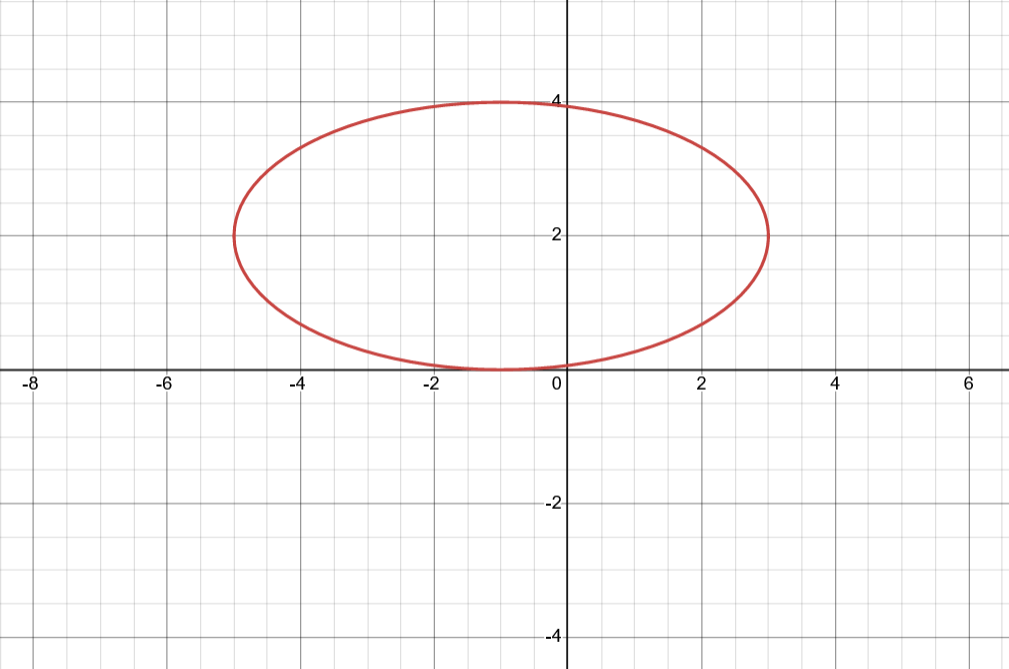
\includegraphics[width=0.5\linewidth]{cox-little-oshea/ch1/assets/sec1-2-ex1a.png}
     \caption{Graph of $\bV(x^2 + 4y^2 + 2x - 16y + 1)$}
     \label{fig:sec1-2-ex1a}
        \end{figure}
        I would expect a dimension of $1$, which the figure does seem to indicate.
        \item This is a union of the lines $x=\pm y$.
        \begin{figure}[H]
            \centering
            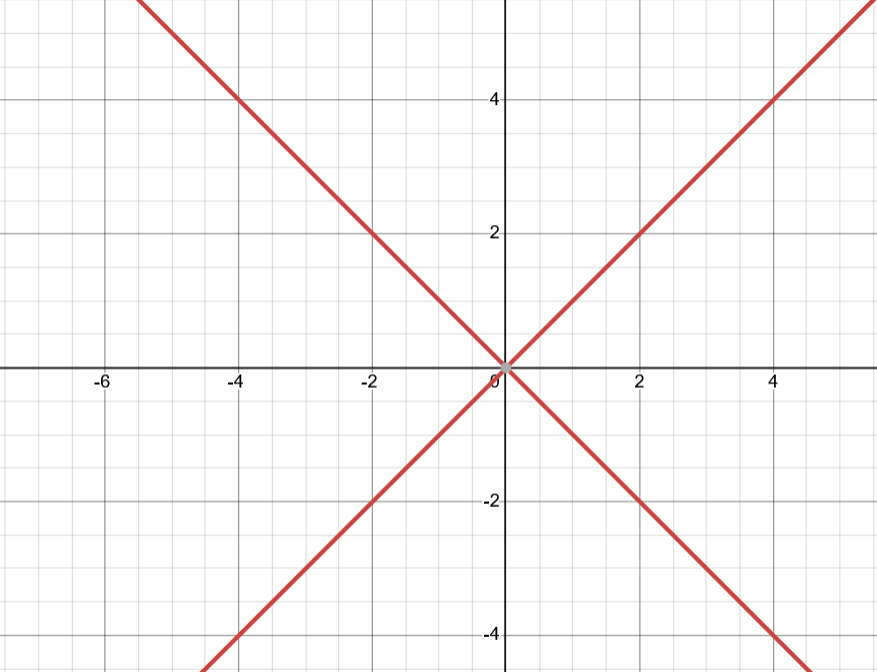
\includegraphics[width=0.5\linewidth]{cox-little-oshea/ch1/assets/sec1-2-ex1b.png}
            \caption{Graph of $\bV(x^2 - y^2)$}
            \label{fig:sec1-2-ex1b}
        \end{figure}
        I would expect a dimension of $1$, which the figure does seem to indicate except perhaps in the origin.
        \item Solving the system
        \begin{align*}
            \left\{\begin{array}{l}
            2x + y - 1 = 0\\
            3x - y + 2 = 0,
        \end{array}\right.
        \end{align*}
        we get as only solution $\parens{-\frac{1}{5},\frac{7}{5}}$. 
        The variety will just be a single point.
        \begin{figure}[H]
            \centering
            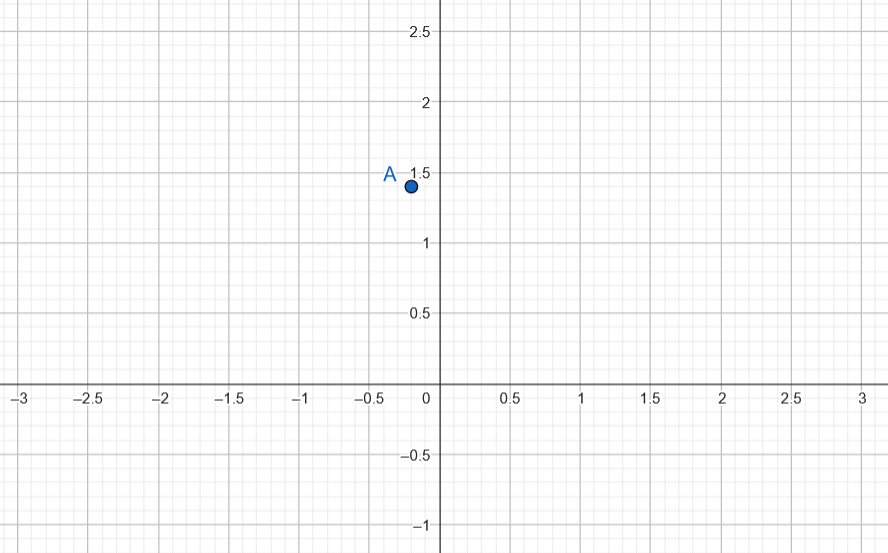
\includegraphics[width=0.5\linewidth]{cox-little-oshea/ch1/assets/sec1-2-ex1c.png}
            \caption{Graph of $\bV(2x+y-1, 3x - y + 2)$}
            \label{fig:sec1-2-ex1c}
        \end{figure}
        I would expect a dimension of $0$, which a single point does have.
    \end{enumerate}
\end{proof}

\begin{exercise}{2}
In $\R^2$, sketch $\bV(y^2-x(x-1)(x-2))$. 
Hint: For which $x$'s is it possible to solve for $y$? 
How many $y$'s correspond to each $x$? 
What symmetry does the curve have?
\end{exercise}
\begin{proof}
I will use a graphing calculator for this exercise, but still will answer the hint questions. 
If we solve for $y$, we obtain $y=\sqrt{x(x-1)(x-2)}$, so that we can solve for $y$, whenever $x(x-1)(x-2)\geq 0$. 
We require that either all of $x, x-1$ and $x-2$ are non-negative, or exactly two of them are negative. 
All of them are non-negative whenever $x\geq 2$ and two of them are negative whenever $0<x<1$. 
For these values of $x$ we have two values of $y$ (positive and negative), and hence we obtain symmetry with respect to the $x$-axis.
 \begin{figure}[H]
     \centering
     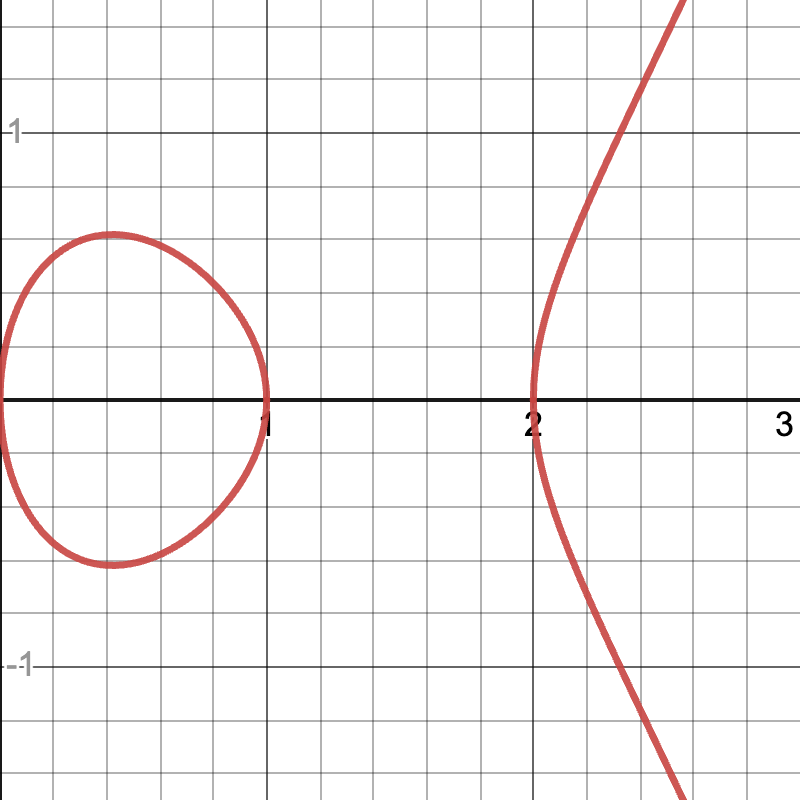
\includegraphics[width=.5\textwidth]{cox-little-oshea/ch1/assets/sec1-2-ex2.png}
     \caption{Graph of $\bV(y^2-x(x-1)(x-2))$}
     \label{fig:sec1-2-ex2}
 \end{figure}
\end{proof}

\begin{exercise}{3}
In the plane $\R^2$, draw a picture to illustrate $\bV(x^2+y^2-4) \cap \bV(xy-1) = \bV(x^2+y^2-4,xy-1)$, and determine the points of intersection. Note that this is a special case of lemma 2.
\end{exercise}
\begin{proof}
 \begin{figure}[H]
     \centering
     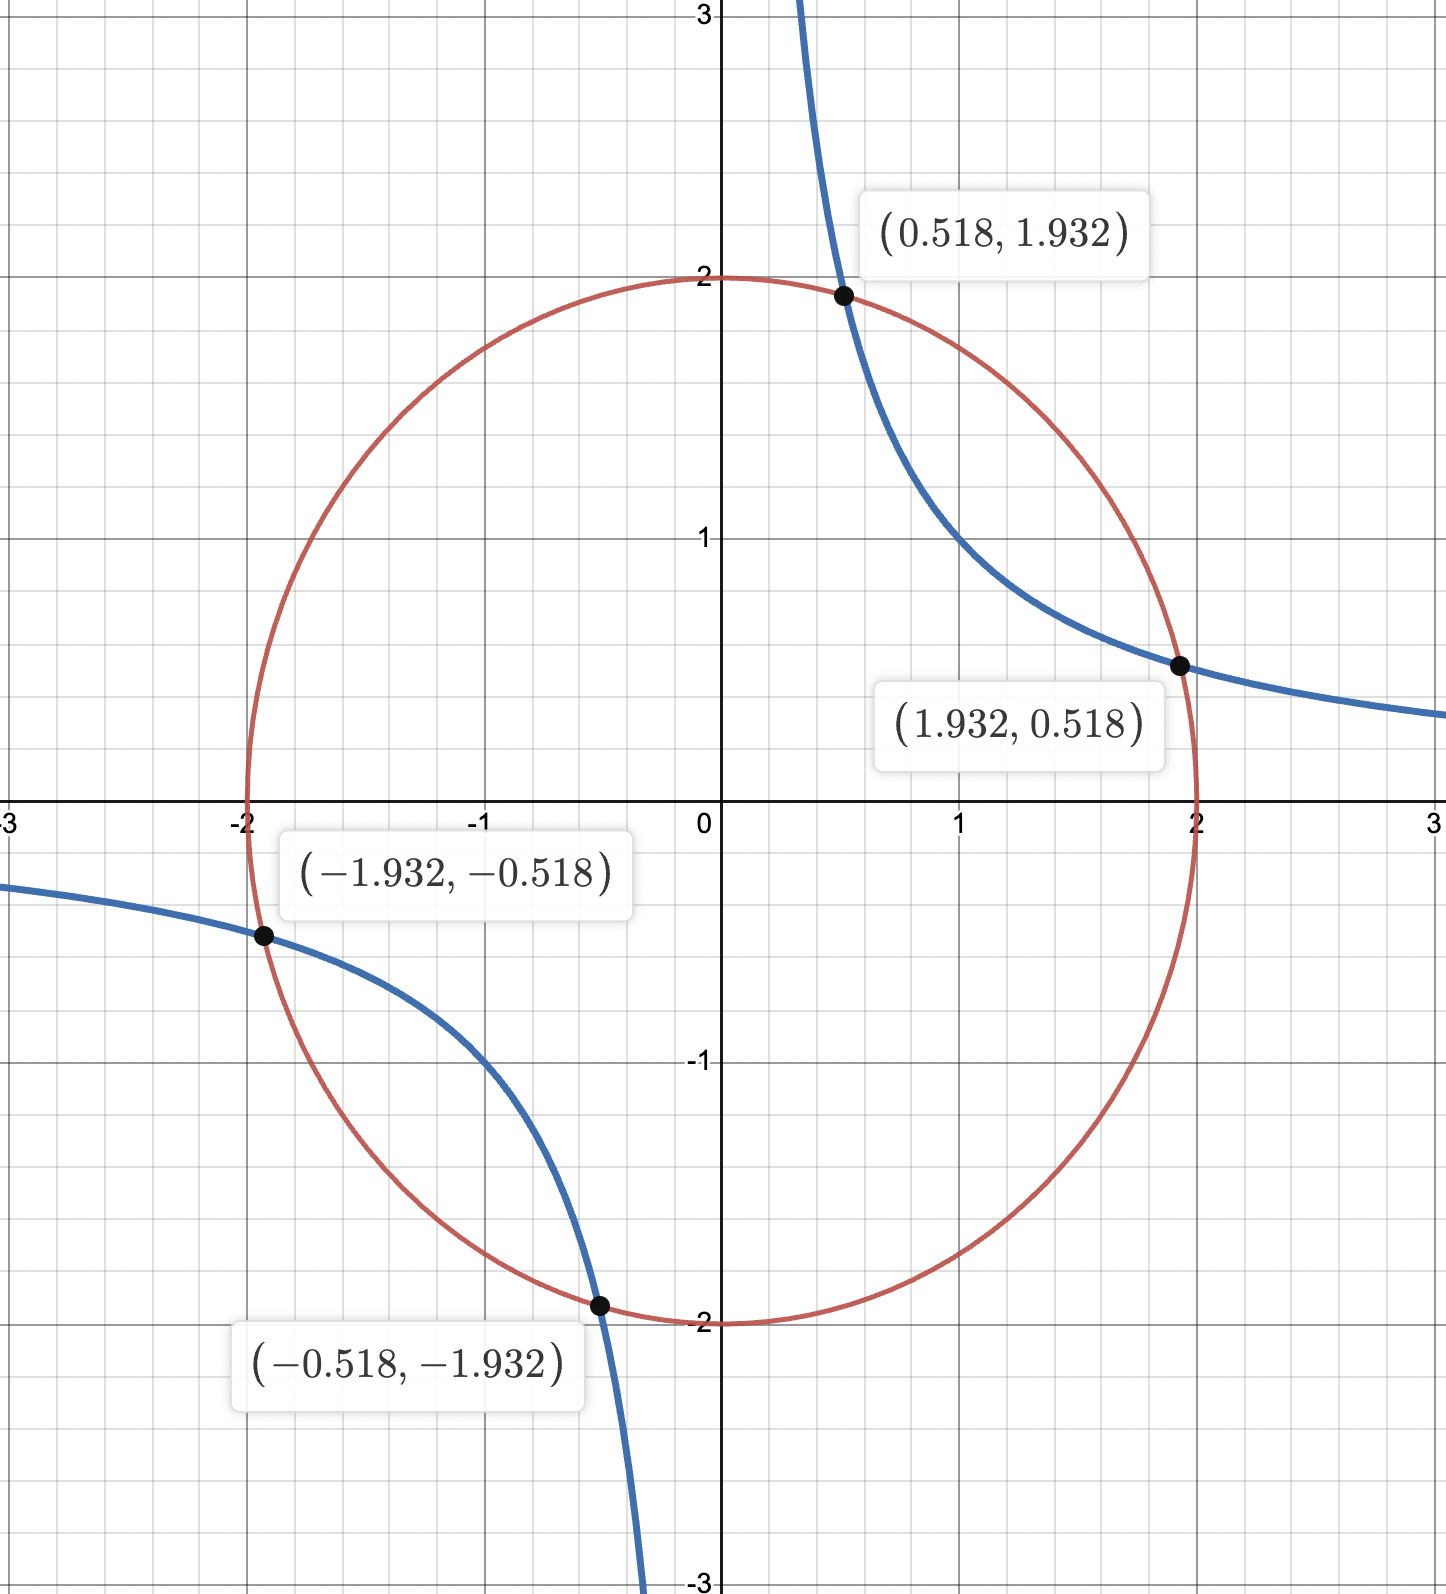
\includegraphics[width=.5\textwidth]{cox-little-oshea/ch1/assets/sec1-2-ex3.png}
     \caption{Graph of $\bV(x^2+y^2-4), \bV(xy-1)$, and its intersection points}
     \label{fig:sec1-2-ex3}
 \end{figure}
\end{proof}

\begin{exercise}{4}
Sketch the following affine varieties in $\R^3$:
\begin{enumerate}
    \item $\bV(x^2 + y^2 + z^2 - 1)$.
    \item $\bV(x^2 + y^2 - 1)$.
    \item $\bV(x+2, y-1.5, z)$.
    \item $\bV(xz^2 - xy)$.
    \item $\bV(x^4 - zx, x^2 - yx)$.
    \item $\bV(x^2 + y^2 + z^2 - 1, x^2 + y^2 + (z-1)^2 - 1)$.
\end{enumerate}
In each case, does the variety have the dimension you would intuitively expect it to have.
\end{exercise}
\begin{proof}
    \begin{enumerate}
        \item This is a sphere of radius $1$.
        \begin{figure}[H]
            \centering
            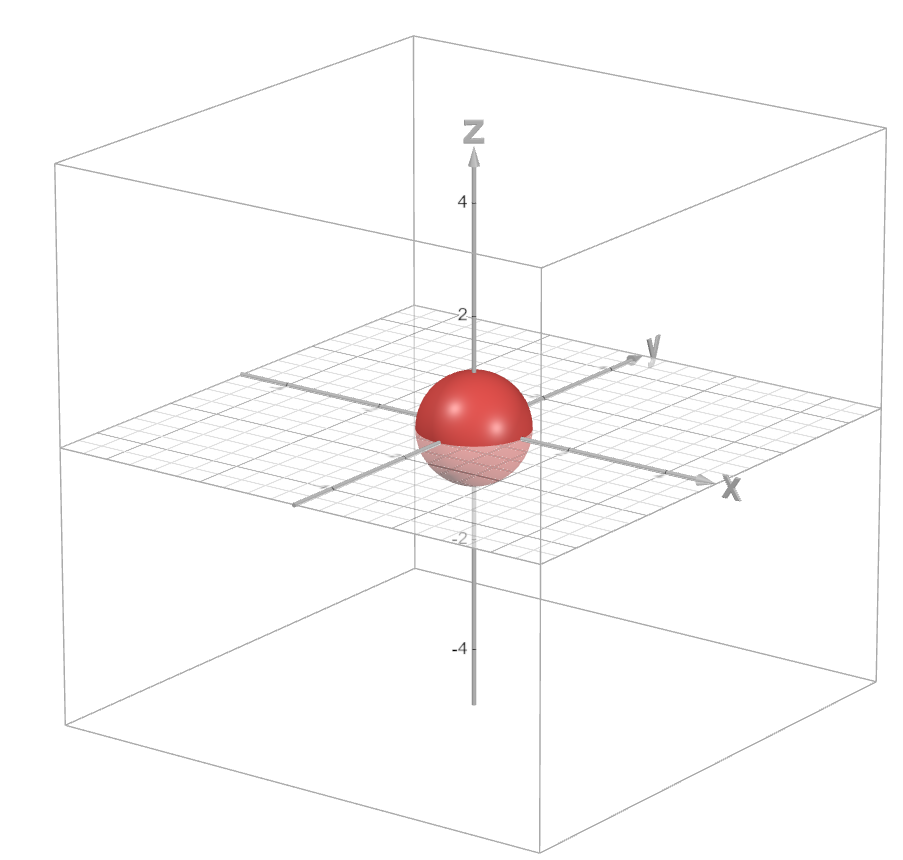
\includegraphics[width=0.5\linewidth]{cox-little-oshea/ch1/assets/sec1-2-ex4a.png}
            \caption{Graph of $\bV(x^2+y^2+z^2-1)$}
            \label{fig:sec1-2-ex4a}
        \end{figure}
        I would expect it to have dimension $2$, which is true.
        \item This is a cylinder of radius $1$.
        \begin{figure}[H]
            \centering
            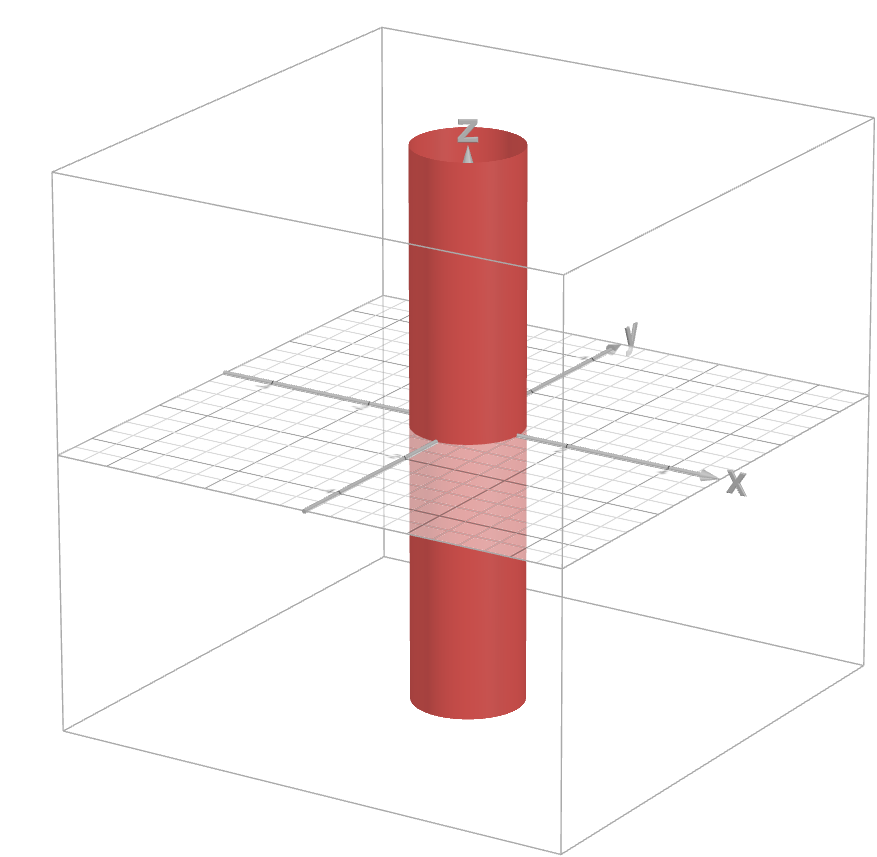
\includegraphics[width=0.5\linewidth]{cox-little-oshea/ch1/assets/sec1-2-ex4b.png}
            \caption{Graph of $\bV(x^2+y^2-1)$}
            \label{fig:sec1-2-ex4b}
        \end{figure}
        I would expect this to have dimension $2$, and it does.
        \item This is simply a point
        \begin{figure}[H]
            \centering
            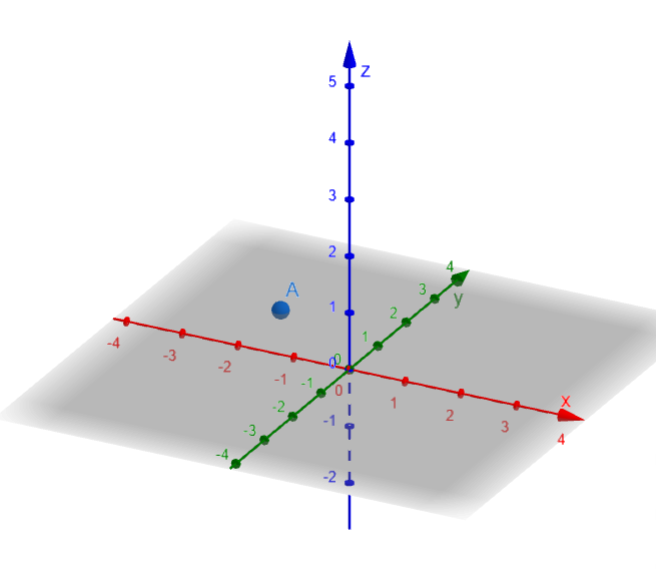
\includegraphics[width=0.5\linewidth]{cox-little-oshea/ch1/assets/sec1-2-ex4c.png}
            \caption{Graph of $\bV(x+2, y-1.5, z)$}
            \label{fig:sec1-2-ex4c}
        \end{figure}
        I would expect this to have dimension $0$ and it does.
        \item This is $\bV(x)\cup \bV(z^2 - y)$. 
        \begin{figure}[H]
            \centering
            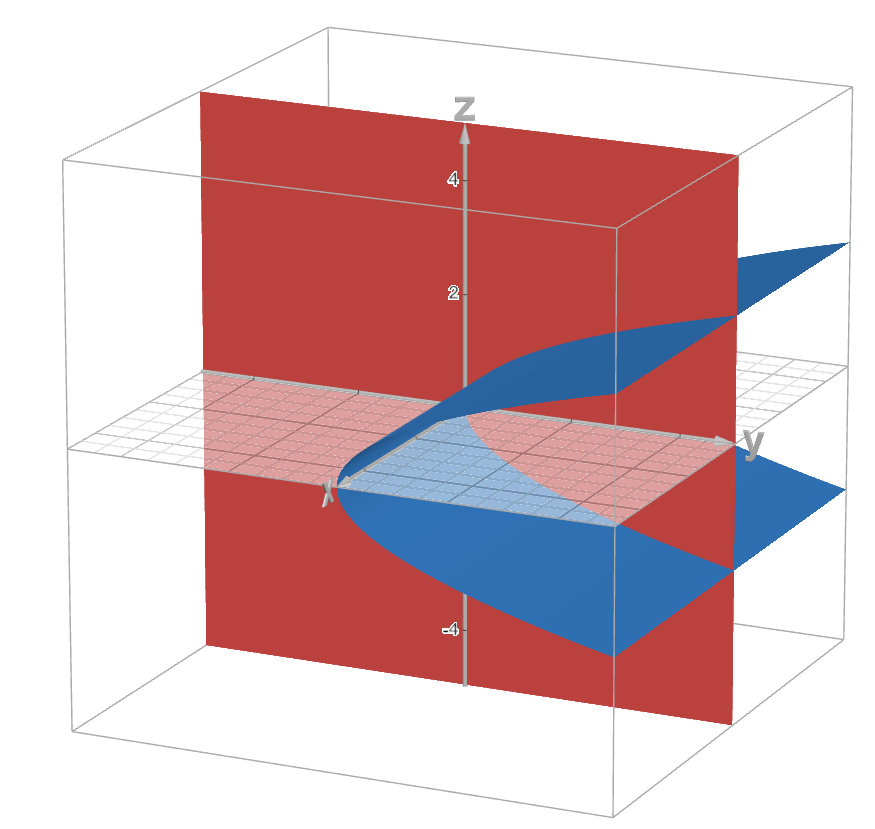
\includegraphics[width=0.5\linewidth]{cox-little-oshea/ch1/assets/sec1-2-ex4d.png}
            \caption{Graph of $\bV(xz^2 - xy)$}
            \label{fig:sec1-2-ex4d}
        \end{figure}
        We expect this to have dimension $2$, and it kind of does except in the intersection points perhaps.
        \item We have to solve
        \begin{align*}
          x(x^3 - z) = 0,~x(x^2 - y) = 0.  
        \end{align*}
        Clearly the equation $x=0$ is a solution. Now assume that $x\neq 0$, then we get the solution curve given by $(t,t^2,t^3)$.
        \begin{figure}
            \centering
            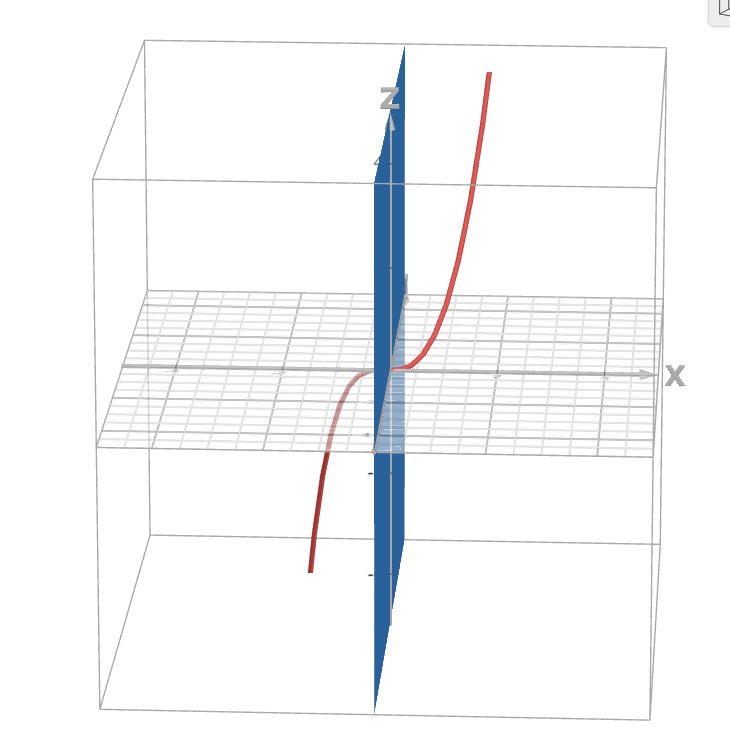
\includegraphics[width=0.5\linewidth]{cox-little-oshea/ch1/assets/sec1-2-ex4e.png}
            \caption{Graph of $\bV(x^4 - zx, x^3 - yx)$}
            \label{fig:sec1-2-ex4e}
        \end{figure}
        We expect this to have dimension $1$, but a lot of the points on the variety have dimension $2$.
        \item We get that
        \begin{align*}
            z^2 = 1 - x^2 - y^2 = (z-1)^2.
        \end{align*}
        Clearly this implies $z=z-1$ or $z=1-z$. The former can never happen, and the latter implies $z = \frac{1}{2}$. 
        We get the equation
        \begin{align*}
            x^2 + y^2 = \frac{3}{4}.
        \end{align*}
        This is a cylinder.
        \begin{figure}
            \centering
            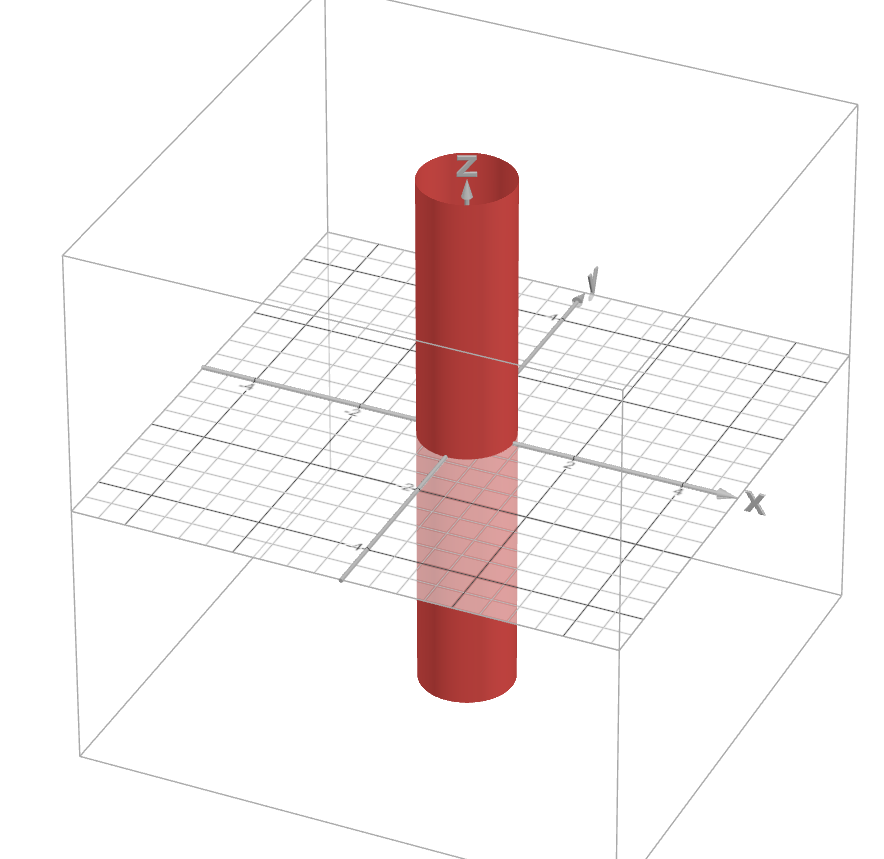
\includegraphics[width=0.5\linewidth]{cox-little-oshea/ch1/assets/sec1-2-ex4f.png}
            \caption{Graph of $\bV(x^2 + y^2 + z^2 - 1, x^2 + y^2 + (z-1)^2 - 1)$}
            \label{fig:sec1-2-ex4f}
        \end{figure}
        We expect this to have dimension $1$, but we get a variety of dimension $2$.
    \end{enumerate}
\end{proof}

\begin{exercise}{5}
Use the proof of Lemma $2$ to sketch $\bV( (x-2)(x^2 - y), y(x^2 - y), (z+1)(x^2-y))$ in $\R^3$.
\end{exercise}
\begin{proof}
    We get that this is
    \begin{align*}
        \bV(x^2 - y)\cup \bV(x-2, y, z+1).
    \end{align*}
    So it is the union of the variety given by equation $y=x^2$ and the point $(2,0,-1)$.
    \begin{figure}
        \centering
        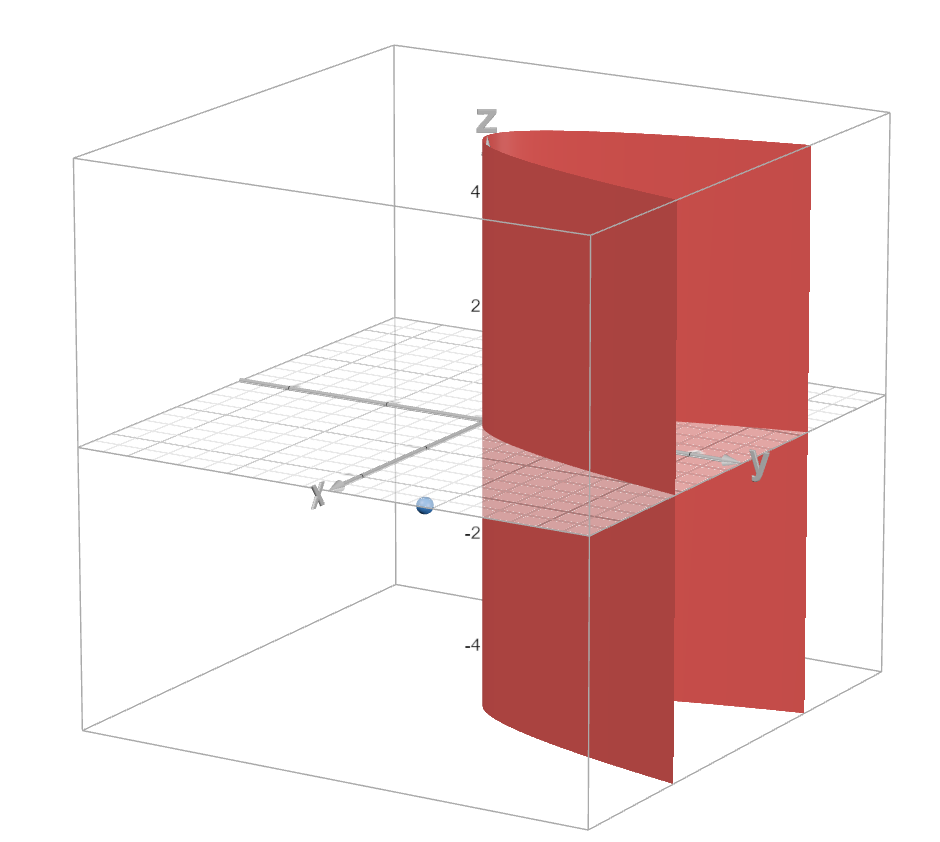
\includegraphics[width=0.5\linewidth]{cox-little-oshea/ch1/assets/sec1-2-ex5.png}
            \caption{Graph of $\bV( (x-2)(x^2 - y), y(x^2 - y), (z+1)(x^2-y))$}
            \label{fig:sec1-2-ex5}
    \end{figure}
\end{proof}

\begin{exercise}{6}
Let us show that all finite subsets of $k^n$ are affine varieties.
\begin{enumerate}
    \item Prove that a single point $(a_1,\dots,a_n)\in k^n$ is an affine variety.
    \item Prove that every finite subset of $k^n$ is an affine variety. 
    Hint: Lemma 2 will be useful.
\end{enumerate}
\end{exercise}
\begin{proof}
 \begin{enumerate}
     \item Consider the set of polynomials $f_1,\dots,f_n$ given by $f_i(x_i)=x_i-a_i$. 
     Then certainly $\bV(f_1,\dots,f_n)$ has as variety the point $(a_1,\dots,a_n)\in k^n$, as required.
     \item We have just proven above that any point is an affine variety of a particular set of polynomials, so that for any point in the set we are interested in, say $(a_{i,1},\dots,a_{i,n})$ is a variety $\bV_i$ of a set of polynomials. 
     From Lemma 2, we know that the union of two varieties is a variety, hence, $\cup_{i=1}^{m}\bV_i$ is a variety.
 \end{enumerate}
\end{proof}

\begin{exercise}{7}
One of the prettiest examples from polar coordinates is the four-leaved rose. 
This curve is defined by the polar equation $r=\sin(2\theta)$. 
We will show that this curve is an affine variety.
\begin{enumerate}
    \item Using $r^2 = x^2 + y^2$, $x=r\cos(\theta)$ and $y=r\sin(\theta)$, show that the four-leaved rose is contained in the affine variety $\bV( (x^2 + y^2)^3 - 4x^2 y^2)$.
    \item Now argue carefully that $\bV((x^2 + y^2)^3 - 4x^2 y^2)$ is contained in the four-leaved rose. 
    This is trickier than it seems since $r$ can be negative in $r=\sin(2\theta)$.
\end{enumerate}
Combining parts (a) and (b), we have proved that the four-leaved rose is the affine variety $\bV((x^2 + y^2)^3 - 4x^2 y^2)$.
\end{exercise}
\begin{proof}
    \begin{enumerate}
        \item We get that
        \begin{align*}
            (x^2 + y^2)^3 - 4x^2 y^2
            = & (r^2)^3 - 4(r\cos\theta)^2 (r\sin\theta)^2\\
            = & r^6 - 4r^4 \cos^2\theta \sin^2\theta\\
            = & r^6 - r^4 \sin^2(2\theta)\\
            = & r^4(r^2 - \sin^2(2\theta))\\
            = & r^4(r-\sin(2\theta))(r+\sin(2\theta))\\
            = & 0.
        \end{align*}
        \item Take a point $(x,y)$ with $(x^2 + y^2)^3 = 4x^2y^2$. We can find some angle $\theta$ such that $(x,y) = (r\cos\theta, r\sin\theta)$. Then,
        \begin{align*}
            0
            = & (x^2 + y^2)^3 - 4x^2 y^2\\
            = & (r^2\cos^2\theta + r^2\sin^2\theta)^3 - 4(r\cos\theta)^2 (r\sin\theta)^2\\
            = & r^6 - 4r^4 \cos^2\theta \sin^2\theta\\
            = & r^6 - r^4 \sin^2(2\theta)\\
            = & r^4 (r^2 - \sin^2(2\theta)).
        \end{align*}
        There are a few possibilities on $r$:
        \begin{itemize}
            \item If $r=0$, then $(x,y) = (0,0)$, but then we can choose $r=0$ and $\theta = 0$ and then the equation $r=\sin(2\theta)$ will be satisfied.
            \item If $r\neq 0$, then $|r| = |\sin(2\theta)|$. 
            If $r = \sin(2\theta)$, the result has been shown. 
            In the other case, we have $r=-\sin(2\theta)$. 
            In that case, we notice that
            \begin{align*}
                -r
                = & \sin(2\theta)\\
                = & \sin(2\theta + 2\pi)\\
                = & \sin(2(\theta + \pi)),
            \end{align*}
            and $(x,y) = (-r\cos(\pi + \theta), -r\sin(\pi + \theta))$, and thus $(x,y)$ also has $r$ and $\theta$ such that $r=\sin(2\theta)$, namely $-r$ and $\pi+\theta$.
        \end{itemize}
    \end{enumerate}
\end{proof}

\begin{exercise}{8}
It can take some work to show that something is not an affine variety. 
For example, consider the set $X=\set{(x,x)\mid x\in\R, x\neq 1}\subseteq\R^2$, which is the straight line $x=y$ with the point $(1,1)$ removed. 
To show that $X$ is not an affine variety, suppose that $X=\bV(f_1,\dots,f_s)$. 
Then each $f_i$ vanishes on $X$, and if we can show that $f_i$ also vanishes at $(1,1)$, we will get the desired contradiction. 
Thus, here is what you are to prove: if $f\in\R[x,y]$ vanishes on $X$, then $f(1,1)=0$. 
Hint: let $g(t)=f(t,t)$, which is a polynomial $\R[t]$. 
Now apply the proof of Proposition 5 of Section 1.
\end{exercise}
\begin{proof}
 If $f_i$ vanishes on $X$, then $f_i$ has infinitely many roots. 
 But we know that a polynomial with infinitely many roots must be the zero polynomial. 
 Hence, $f_i=0$ and $f_i(1,1)=0$, as required.
\end{proof}

\begin{exercise}{9}
Let $R = \set{(x,y)\in \R^2~\vert~y>0}$ be the upper half plane. 
Prove that $R$ is not an affine variety.
\end{exercise}
\begin{proof}
    Assume that $R = \bV(f_1,...,f_s)$. 
    Then each $f_i$ vanishes on $R$. 
    Let $f\in \R[x,y]$ be any polynomial vanishing on $R$, then take $g(t) = f(a+t,t)$. 
    We see that $g$ is a polynomial with infinitely many zeroes. 
    Since $\R$ is an infinite field, we must then have $g = 0$. 
    Thus for all $a,t\in \R$, we must have $f(a+t,t) = 0$. 
    Thus $f = 0$ on $R$. 
    In particular, we see that $f_1 = ... = f_s = 0$. 
    Thus $R = \bV(f_1,...,f_s) = \R^2$, which is a contradiction.
\end{proof}

\begin{exercise}{10}
Let $\Z^n\subseteq \C^n$ consists of those points with integer coordinates. 
Prove that $\Z^n$ is not an affine variety.    
\end{exercise}
\begin{proof}
    Write $\Z^n = \bV(f_1,...,f_s)$. 
    For every $i$ then, we see that $f_i$ vanishes at all points of $\Z^n$. 
    By exercise 1.6, we see then that $f_i = 0$. This holds for arbitrary $i$, hence
    \begin{align*}
        \Z^n = \bV(0) = \C^n,
    \end{align*}
    a contradiction.
\end{proof}

\begin{exercise}{11}
So far we have discussed varieties of $\R$ or $\C$. 
It is also possible to consider varieties over the field $\Q$, although the questions here tend to be much harder. 
For example, let $n$ be a positive integer, and consider the variety $F_n\subseteq\Q^2$ defined by $x^n+y^n=1$. 
Notice that there are some obvious solutions when $x$ or $y$ is zero. 
We call these trivial solutions. 
An interesting question is whether or not there are nontrivial solutions.
\begin{enumerate}
    \item Show that $F_n$ has two trivial solutions if $n$ is odd and four trivial solutions if $n$ is even.
    \item Show that $F_n$ has a nontrivial solution for some $n\geq 3$ if and only if Fermat's Last Theorem were false.
\end{enumerate}
Fermat's Last Theorem states that, for $n\geq 3$, the equation $x^n+y^n=z^n$ has no solutions where $x,y$ and $z$ are nonzero integers. 
The general case of this conjecture was proved by Andrew Wiles in 1994 using some very sophisticated number theory. 
The proof is extremely difficult.
\end{exercise}
\begin{proof}
    \begin{enumerate}
        \item Odd $n$. 
        The trivial solutions are characterised by $x=0$ or $y=0$. 
        Without loss of generality, suppose $x=0$. Since $n$ is odd, if $y=-1$, then $y^n=-1$ so that the equation is not satisfied. 
        Hence $y$ must be equal to 1. 
        We can conclude the same for $x$ if $y=0$. 
        So that there are 2 trivial solutions in total.

        Even $n$. 
        We can follow the same approach as above. 
        Simply notice that if $x=0$ and $y=-1$, we have that $y^n=1$ so that  $y=\pm1$ are valid solutions. 
        We can reason the same for $x$ when $y=0$ so that we obtain 4 trivial solutions.
        \item ($\Rightarrow$) Suppose $F_n$ has a nontrivial solution. 
        Then there exist $x/p,y/q\in\Q$ and $x,p,y,q\in\Z$ such that $(x/p)^n+(y/q)^n = 1$. 
        Let $k=\lcm(p,q)$, so that $k\in\Z$. 
        Then $(xq)^n+(yp)^n=k^n$. 
        Since $n\geq 3$ and $xq,yp,k\in\Z$ the equation from the previous sentence would imply that Fermat's Last Theorem is false.

        ($\Leftarrow$) Suppose Fermat's Last Theorem is false. 
        Then there exist $x,y,z\in\Z$ such that $x^n+y^n=z^n$ for some $n\geq 3$. 
        However, this implies $(x/z)^n+(y/z)^n=1$. 
        That is, $p^n+q^n=1$, where $p,q\in\Q$, as required.
    \end{enumerate}
\end{proof}

\begin{exercise}{12}
    Find a Lagrange multipliers problem in a calculus book and write down the corresponding system of equations. 
    Be sure to use an example where one wants to find the minimum or maximum of a polynomial function subject to a polynomial constraint. 
    This way the equations define an affine variety, and try to find a problem that leads to complicated equations. 
    Later we will use the Gr\"obner basis methods to solve these equations.
\end{exercise}
\begin{proof}
    Consider the following problem:

    The sum of the lengths of $12$ edges of a rectangular block is $a$; 
    the sum of the area of the $6$ faces is $a^2/25$. 
    Calculate the lengths of the edges when the excess of the volume of the block over that of a cube, whose edges is equal to the least edge of the block, is greatest.

    Let the edges of the block be $e\leq f\leq g$. 
    We need to maximize
    \begin{align*}
        efg - e^3,\, \text{ subject to }\, 4(e+f+g) = a,~~2(ef + eg + fg) = \frac{a^2}{25}.
    \end{align*}
    We get the following equations:
    \begin{align*}
        &fg - 3e^2 &&= 4\lambda + 2\lambda' (f+g),\\
        &eg &&= 4\lambda + 2\lambda' (e+g),\\
        &ef &&= 4\lambda + 2\lambda' (e+f).
    \end{align*}
    
\end{proof}

\begin{exercise}{13}
Consider a robot arm in $\R^2$ that consists of three arms of lengths $3$, $2$, and $1$, respectively. 
The arm of length $3$ is anchored at the origin, the arm of length $2$ is attached to the free end of the arm of length $3$, and the arm of length $1$ is attached to the free end of the arm of length $2$. 
The ``hand'' of the robot arm is attached to the of the arm of length $1$.
\begin{enumerate}
    \item Draw a picture of the robot arm.
    \item How many variables does it take to determine the ``state'' of the robot arm?
    \item Give the equations for the variety of possible states.
    \item Using the intuitive notion of dimension discussed in this section, guess what dimension of the variety of states should be.
\end{enumerate}
\end{exercise}
\begin{proof}
    \begin{enumerate}
        \item 
\begin{figure}[H]
        \centering
        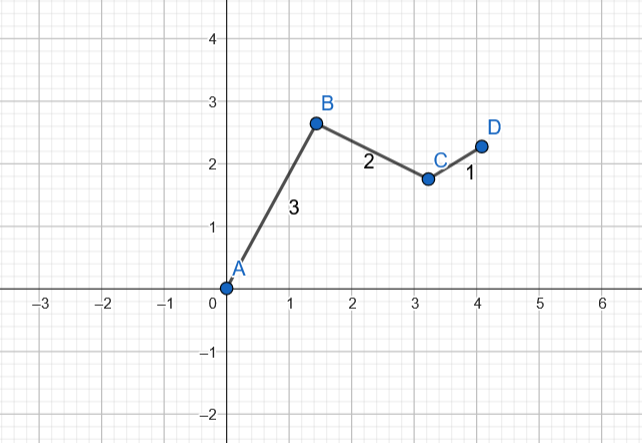
\includegraphics[width=0.5\linewidth]{cox-little-oshea/ch1/assets/sec1-2-ex13.png}
        \caption{An example position of the robot arm}
        \label{fig:sec1-2-ex13}
    \end{figure}
    \item It takes $3$ variables: 
    the angle of each arm with the $x$-axis.
    \item To describe the first arm, we have
    \begin{align*}
        x^2 + y^2 = 9.
    \end{align*}
    To describe the second arm, we have
    \begin{align*}
        (a-x)^2 + (b-y)^2 = 4.
    \end{align*}    
    To describe the third arm, we have
    \begin{align*}
        (u-a)^2 + (v-b)^2 = 1.
    \end{align*}
    \item There are $3$ equations in (c) with a total of $6$ variables. 
    We expect the dimension to be $6-3 = 3$. 
    This is in line with (b).
\end{enumerate}
\end{proof}

\begin{exercise}{14}
This exercise will study the possible ``hand'' positions of the robot arm described in Exercise $13$.
\begin{enumerate}
    \item If $(u,v)$ is the position of the hand, explain why $u^2 + v^2 \leq 36$.
    \item Suppose we ``lock the joint between the length $3$ and length $2$ arms to form a straight angle, but allow the other joint to move freely. 
    Draw a picture to show that in these configurations, $(u,v)$ can be any point of the annulus $16\leq u^2 + v^2 \leq 36$.
    \item Draw a picture to show that $(u,v)$ can be any point in the disk $u^2 + v^2\leq 36$.
\end{enumerate}
\end{exercise}
\begin{proof}
    \begin{enumerate}
        \item The furthest the hand gets from the origin is when all three arms are on one line. 
        To find how far the hand is, it suffices to add the lengths of the three arms to get $3+2+1 = 6$. 
        Thus $(u,v)$ must always be a distance $6$ or less away from the origin, leading to $u^2 + v^2 \leq 36$.
        \item We get
        \begin{figure}[H]
            \centering
            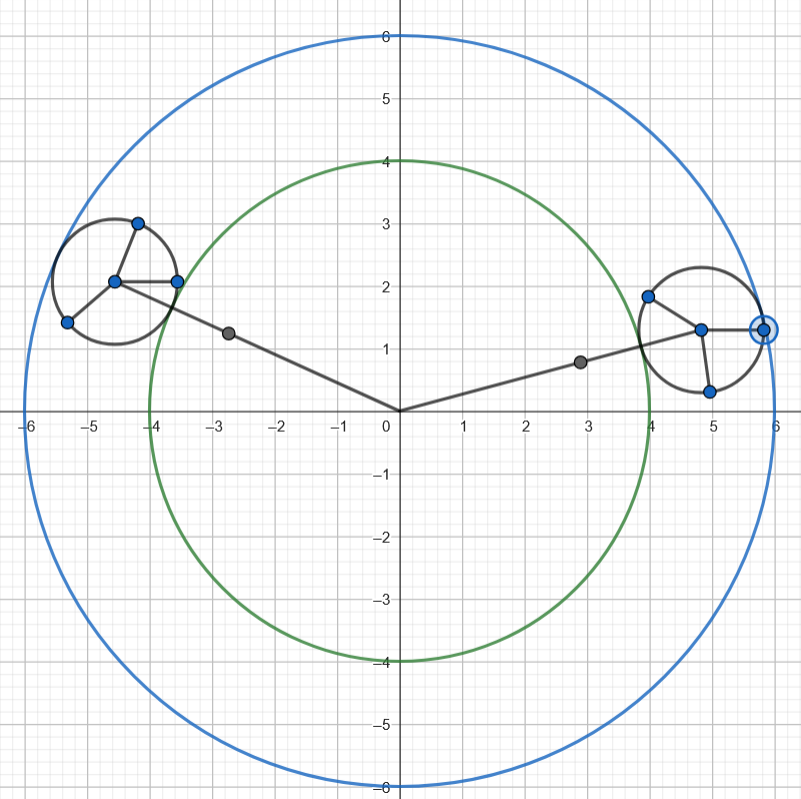
\includegraphics[width=0.5\linewidth]{cox-little-oshea/ch1/assets/sec1-2-ex14b.png}
            \caption{Some different configurations of the arm with one joint locked.}
            \label{fig:sec1-2-ex14b}
        \end{figure}
        \item The case $16\leq u^2 + v^2\leq 36$ has already been done in part (b). 
        For $4\leq u^2 + v^2\leq 16$, we fold the length $1$ arm onto the length $2$ arm and lock the joint. 
        We effectively get an arm of length $1$ at the end of an arm of length $3$. 
        \begin{figure}
            \centering
            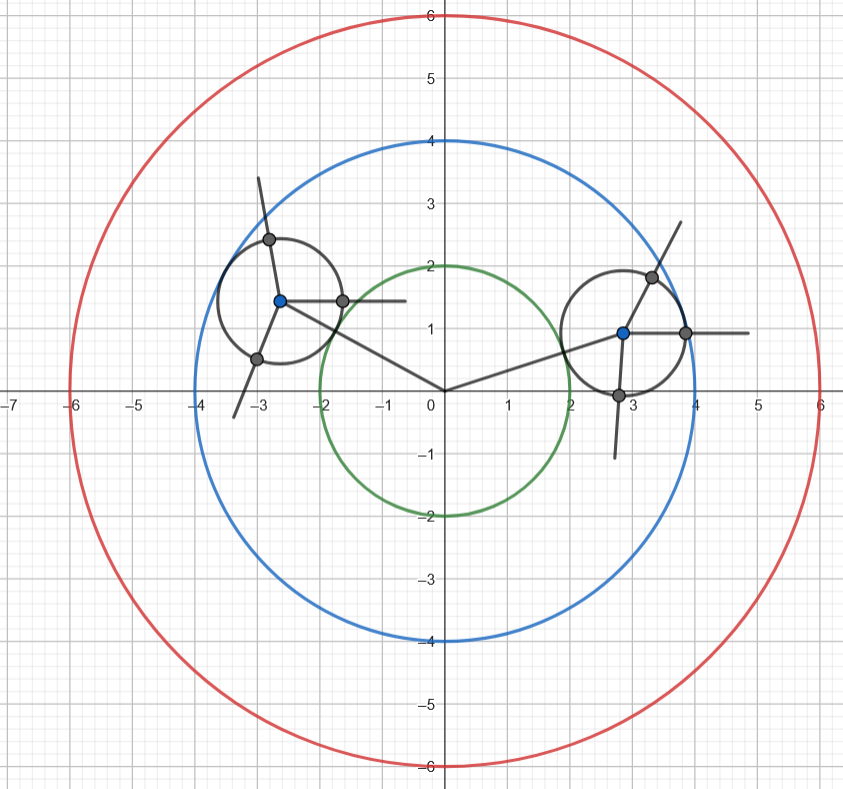
\includegraphics[width=0.5\linewidth]{cox-little-oshea/ch1/assets/sec1-2-ex14c.png}
            \caption{Some different configurations of the arm with one joint locked and folded in.}
            \label{fig:sec1-2-ex14c}
        \end{figure}
        For $leq u^2 + v^2\leq 4$, we fold the length $2$ arm onto the length $3$ arm and lock the joint. 
        We effectively get an arm of length $1$ at the end of an arm of length $1$. 
        \begin{figure}
            \centering
            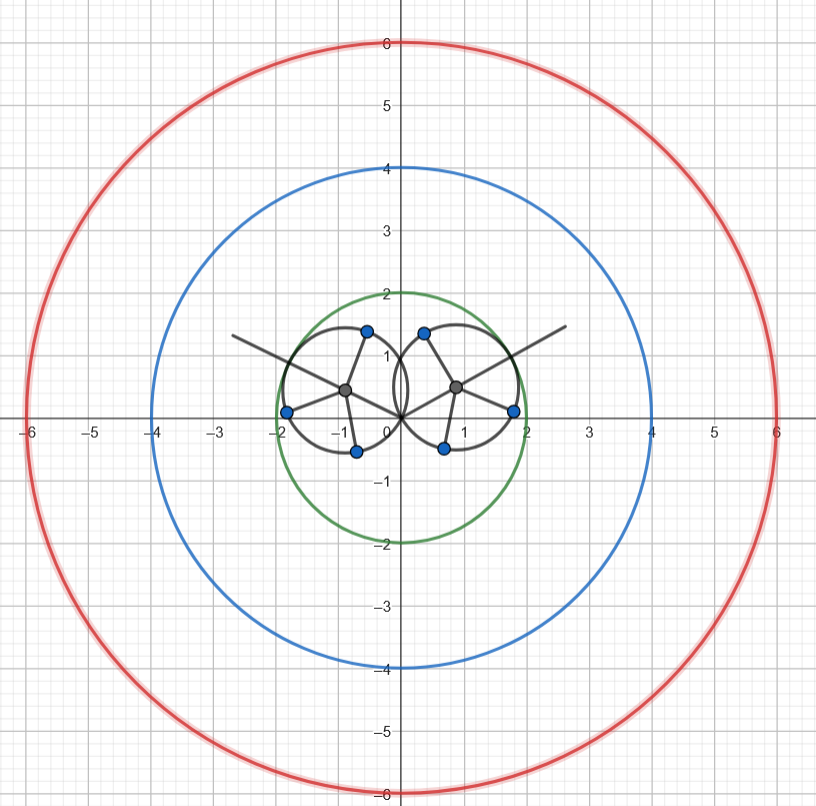
\includegraphics[width=0.5\linewidth]{cox-little-oshea//ch1/assets/sec1-2-ex14c2.png}
            \caption{Some different configurations of the arm with one joint locked and folded in.}
            \label{fig:sec1-2-ex14c2}
        \end{figure}
    \end{enumerate}
\end{proof}

\begin{exercise}{15}
In Lemma 2, we showed that if $V$ and $W$ are affine varieties, the so are their union $V\cup W$ and intersection $V\cap W$. 
In this exercise we will study how other set-theoretic operations affect affine varieties.
\begin{enumerate}
    \item Prove that finite unions and intersections of affine varieties are again affine varieties. 
    Hint: Induction.
    \item Give an example to show that an infinite union of affine varieties need not be an affine variety. 
    Hint: By exercises 8-10, we know some subset of $k^n$ that are not affine varieties. 
    Surprisingly, an infinite intersection of affine varieties is still an affine variety. 
    This is a consequence of the Hilbert Basis Theorem, which will be discussed in Chapters 2 and 4.
    \item Given an example to show that the set-theoretic difference $V\setminus W$ of two affine varieties need not be an affine variety.
    \item Let $V\subseteq k^n$ and $W\subseteq k^m$ be two affine varieties, and let $V\times W = \set{(x_1,\dots,x_n,y_1,\dots,y_m)\in k^{n+m}\mid(x_1,\dots,x_n)\in V,(y_1,\dots,y_m)\in W}$ be their Cartesian product. 
    Prove that $V\times W$ is an affine variety in $k^{n+m}$. 
    Hint: If $V$ is defined by $f_1,\dots,f_s\in k[x_1,\dots,x_n]$, then we can regard $f_1,\dots,f_s$ as polynomials in $k[x_1,\dots,x_n,y_1,\dots,y_m]$, and similarly for $W$. Show that this gives defining equations for the Cartesian product.
\end{enumerate}
\end{exercise}
\begin{proof}
    \begin{enumerate}
        \item We will prove by induction that finite unions of affine varieties are again affine varieties. 
        The result for intersections can be proved in a similar manner. 

        Base case: 
        the result in Lemma 2. 
        Now suppose the result holds for the union of $n-1$ affine varieties, so that $\cap_{i=1}^{n-1}\bV_i$ is an affine variety. 
        From Lemma 2, we know that $\cap_{i=1}^{n-1}\bV_i= \bV= {\set{f_1^1,\dots f_{s_1}^1,f_1^2,\dots,f_{s_2}^2,\dots,f_1^{n-1},\dots,f_{s_{n-1}}^{n-1}}}$, where $f_i^j$ corresponds to the $i$-th polynomial of the $j$-th affine variety. 
        Certainly, $\cap_{i=1}^{n-1}\bV_i\cap \bV_n$ is an affine variety where $\cap_{i=1}^{n-1}\bV_i\cap \bV_n = \bV=\set{f_1^1,\dots,f_{s_{n-1}}^{n-1},f_1^n,\dots,f_{s_n}^n}$, as required.
        \item In Exercise 6, we proved that any single point in $k^n$ is an affine variety. 
        Consider the infinite union of single points $(x,x)$ where $x \in \R \setminus \set{1}$. 
        Then we obtain the set $X=\set{(x,x)\mid x\in\R,x\neq 1}$, which we proved in exercise 8, is not an affine variety.
        \item Consider the affine variety given by $X'=\set{(x,x)\mid x\in\R}$ and the set $\set{(1,1)}$. 
        We have $X=X'\setminus\set{(1,1)}$, which we proved is not an affine variety.
        \item Following the hint, we consider $f_1,\dots,f_s,g_1,\dots,g_t\in k[x_1,\dots,x_n,y_1,\dots,y_m]$. 
        We then have that for any $(x_1,\dots,y_m)\in V\times W$, and any $h_i \in \set{f_1,\dots,f_s,g_1,\dots,g_t}$, $h_i(x_1,\dots,y_m)=0$, given that, if $h_i=f_j$ for some $j$, then $f_j(x_1,\dots,y_m)=0$ by virtue of $(x_1,\dots,x_n)\in V$ and likewise for $h_i=g_j$. 
        Then, $V\times W$ is an affine variety, where the defining polynomials are $\set{f_1,\dots,f_s,g_1,\dots,g_t}\in k[x_1,\dots,x_n,y_1,\dots,y_m]$, as required.
    \end{enumerate}
\end{proof}
\section{Parametrizations of Affine Varieties}


\begin{exercise}{1}
Parametrize all solutions of the linear equations
\begin{eqnarray*}
    x + 2y - 2z + w & = & -1\\
    x + y + z - w & = & 2.
\end{eqnarray*}
\end{exercise}
\begin{proof}
    By subtracting the two equations, we get
    $$y - 3z + 2w = -3.$$
    So taking $z$ and $w$ as parameters, we get
    $$y = 3z - 2w - 3$$
    and
    \begin{eqnarray*}
        x
        & = & 2 - y - z +w\\
        & = & 2 -3z +2w + 3 -z + w\\
        & = & 5 - 4z + 3w.
    \end{eqnarray*}
    We get the parametrization:
    \begin{eqnarray*}
        x & = & -4t + 3s + 5\\
        y & = & 3t + 2s - 3\\
        z & = & t\\
        w & = & s.
    \end{eqnarray*}
\end{proof}

\begin{exercise}{2}
    Use a trigonometric identity to show that
    \begin{eqnarray*}
        x & = & \cos(t),\\
        y & = & \cos(2t)
    \end{eqnarray*}
    parametrizes a portion of a parabola. Indicate exactly what portion of the parabola is covered.
\end{exercise}
\begin{proof}
    We see that for a certain $t$ that
    $$y = \cos(2t) = 2\cos^2(t) - 1 = 2x^2 - 1.$$
    Furthermore, we know that $\cos(t)\in [-1,1]$. So we know that $(\cos(t), \cos(2t))$ always lies in the portion of the parabola $y = 2x^2 -1$ where $x\in [-1,1]$.\\
    Conversely, take some $(x,y)$ with $x\in [-1,1]$ and $y = 2x^2 - 1$. Then we know that there is some $t$ such that $x=\cos(t)$. Then,
    $$y = 2x^2 - 1 = 2\cos^2(t) - 1 = \cos(2t).$$
\end{proof}

\begin{exercise}{3}
Given $f\in k[x]$, find a parametrization of $\bV(y - f(x))$.
\end{exercise}
\begin{proof}
    A parametrization is clearly given by
    \begin{eqnarray*}
        x & = & t\\
        y & = & f(t).
    \end{eqnarray*}
\end{proof}

\begin{exercise}{4}
Consider the parametric representation
\begin{align*}
    x=\frac{t}{1+t},\,\,y=1-\frac{1}{t^2}.
\end{align*}
\begin{enumerate}
    \item Find the equation of the affine variety determined by the above parametric equations.
    \item Show that the above equations parametrize all points of the variety found in part (1) except for the point $(1,1)$.
\end{enumerate}
\end{exercise}
\begin{proof}
\begin{enumerate}
    \item We have 
    \begin{align*}
        &x = \frac{t}{1+t} &&\iff\\
        &x(1+t) = t &&\iff\\
        &x = t(1-x) &&\iff\\
        &t = \frac{x}{1-x},
    \end{align*}
    so that replacing in the equation of $y$ we obtain the equation of the affine variety
    \begin{align*}
        y =& 1 -\frac{1}{\left(\frac{x}{1-x}\right)^2}\\
        =& 1-\frac{(1-x)^2}{x^2}\\
        =& \frac{x^2-1+2x-x^2}{x^2}\iff\\
        &yx^2-2x+1=0.
    \end{align*}
    \item To show this, we simply replace the parametrised equation for $x$ and $y$ in the equation of the affine variety
    \begin{align*}
        &\parens{1-\frac{1}{t^2}}\parens{\frac{t}{1+t}}^2-2\parens{\frac{t}{1+t}}+1=0\\
        &\parens{\frac{t^2(t^2-1)}{t^2(1+t)^2}}-2\parens{\frac{t^3(1+t)}{t^2(1+t)^2}}+1=0\\
        &\parens{\frac{t^4-t^2-2t^3-2t^4}{t^2(1+t)^2}}+1=0\\
        &\frac{t^4-t^2-2t^3-2t^4+t^2(1+t)^2}{t^2(1+t)^2}=0\\
        &\frac{t^4-t^2-2t^3-2t^4+t^2(1+2t+t^2)}{t^2(1+t)^2}=0\\
        &\frac{t^4-t^2-2t^3-2t^4+t^2+2t^3+t^4)}{t^2(1+t)^2}=0\\
        &0=0.
    \end{align*}
    Notice, however, that if $x=1$, then $1=t/(1+t)$ so that $1+t=t$ which is a contradiction.
\end{enumerate}
\end{proof}

\begin{exercise}{5}
    This problem will be concerned with the hyperbola $x^2 - y^2 = 1$.
    \begin{enumerate}
        \item Just as trigonometric functions are used to parametrize the circle, hyperbolic functions are used to parametrize the hyperbola. Show that the point
        \begin{eqnarray*}
            x & = & \cosh(t),\\
            y & = & \sinh(t)
        \end{eqnarray*}
        always lies on $x^2 - y^2 = 1$. What portion of the hyperbola is covered?
        \item Show that a straight line meets a hyperbola in $0$, $1$ or $2$ points, and illustrate your answer with a picture.
        \item Adapt the argument given at the end of the section to derive a parametrization of the hyperbola.
        \item The parametrization you found in in part (c) is undefined for two values of $t$. Explain how this relates to the asymptotes of the hyperbola.
    \end{enumerate}
\end{exercise}
\begin{proof}
    \begin{enumerate}
        \item We see indeed that
        \begin{eqnarray*}
            x^2 - y^2
            & = & \cosh^2 t - \sinh^2 t\\
            & = & 1.
        \end{eqnarray*}
        We claim furthermore, that the part of the hyperbola that is covered is the right branch, where $x\geq 1$. One part of this is clear, since $\cosh t\geq 1$ for all $t\in \mathbb{R}$. Now, given any point with $x\geq 1$. There is a $t$ such that $x=\cosh t$. Then since
        $$y^2 = x^2 - 1 = \cosh^2 - 1 = \sinh^2 t.$$
        Thus we see that $y = \pm \sinh t$. By changing sign of $t$ is necessary, we see indeed that $x=\cosh t$ and $y = \sinh t$.
        \item Let us consider first vertical lines of the form $x=a$. Then,
        \begin{eqnarray*}
            1
            & = & x^2 - y^2\\
            & = & a^2 - y^2.
        \end{eqnarray*}
        We get $y^2 = a^2 - 1$. This has $0$, $1$, or $2$ solution depending on whether $a^2 > 0$, $a^2 = 0$ or $a^2 < 0$. This is illustrated in the following picture:
        \begin{figure}[H]
            \centering
            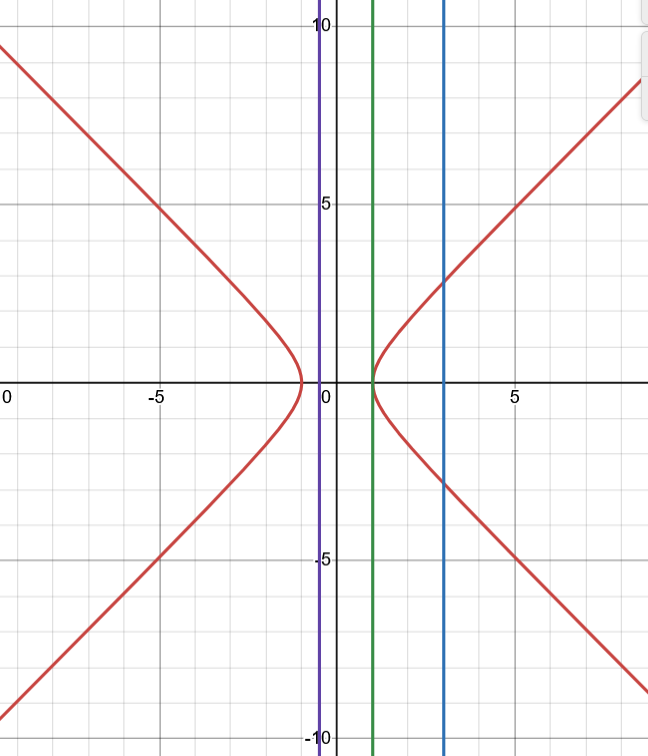
\includegraphics[width=0.5\linewidth]{cox-little-oshea/ch1/assets/sec1-3-ex5b.png}
            \caption{The hyperbola with the vertical lines $x=3$, $x=1$ and $x=1/2$.}
            \label{fig:sec1-3-ex5b}
        \end{figure}
        Next, we have the case of a nonvertical line $y=mx+b$. We get:
        \begin{eqnarray*}
            1
            & = & x^2 - y^2\\
            & = & x^2 - (mx+b)^2\\
            & = & x^2 - m^2 x^2 - 2mbx - b^2\\
            & = & (1 - m^2)x^2 - 2mbx - b^2.
        \end{eqnarray*}
        We get the quadratic equation
        $$(1-m^2)x^2 - 2mbx -(b^2 + 1) = 0.$$
        We have the discriminant
        $$D = 4m^2 b^2 + 4(1-m^2)(b^2 + 1).$$
        According to whether this is positive, negative, or zero, we see that the lines have zero, one or two solutions. This is illustrated in the following picture
\begin{figure}
    \centering
    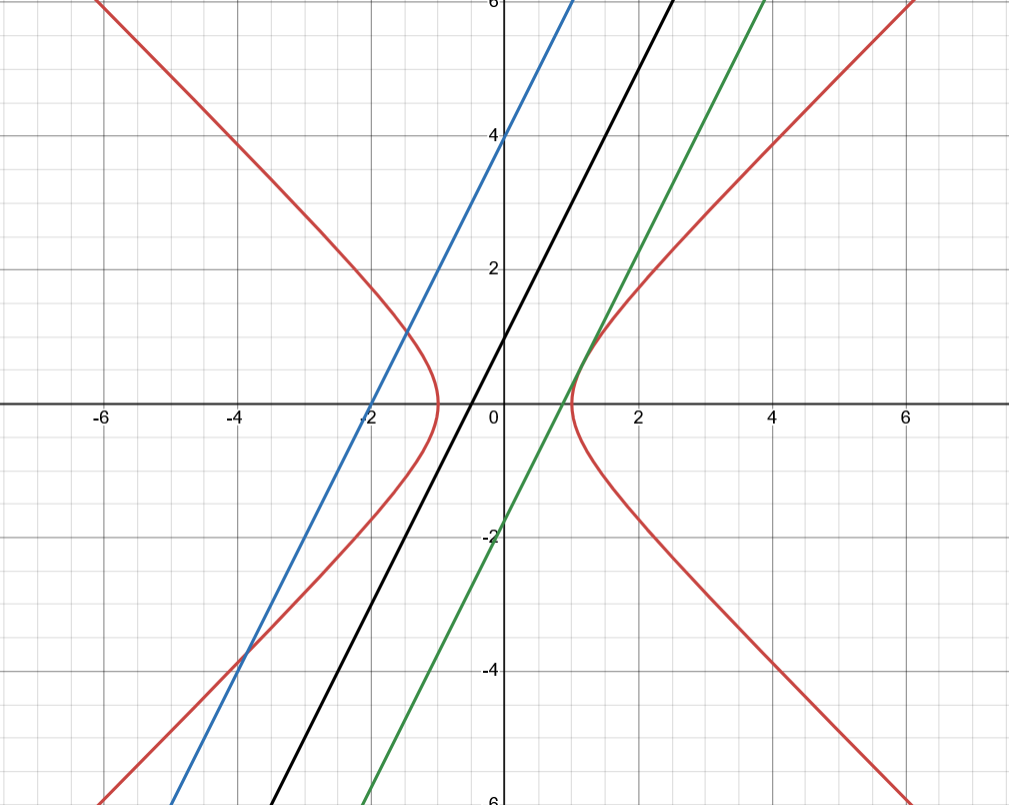
\includegraphics[width=0.5\linewidth]{cox-little-oshea/ch1/assets/sec1-3-ex5bb.png}
            \caption{The hyperbola with the lines $y = 2x+1$, $y=2x+4$ and $y = 2x-\sqrt{3}$.}
            \label{fig:sec1-3-ex5bb}
\end{figure}
        \item Let us consider a nonvertical line through the point $(-1,0)$ on the hyperbola. Such a line as the form $y = mx + m$. Let us plug this into the equation of the hyperbola:
        \begin{eqnarray*}
            1
            & = & x^2 - y^2\\
            & = & x^2 - (mx+m)^2\\
            & = & x^2 - m^2 x^2 - 2m^2 x - m^2\\
            & = & (1 - m^2) x^2 - 2m^2 x - m^2.
        \end{eqnarray*}
        Thus, we get the quadratic equation
        $$0 = (1 - m^2) x^2 - 2m^2 x - (m^2 + 1) = (x+1)( (1 - m^2)x-(1+m^2) ).$$
        The two intersection points are thus for $x=-1$ and
        $$x = \frac{1 + m^2}{1 - m^2}.$$
        We get then that
        $$y = mx+m = m\frac{1+m^2 + 1-m^2}{1-m^2} = \frac{2m}{1-m^2}.$$
        We get the following parametrization:
        $$x = \frac{1 + t^2}{1-t^2},~~y = \frac{2t}{1-t^2}.$$
        \item The parametrization is undefined for $1-t^2 = 0$, and thus $t=\pm 1$. This corresponds to the lines $y=x+1$ and $y=-x-1$. These lines are parallel to the asymptotes of the hyperbola. The line will as such not intersect the hyperbola at any other point than $(-1,0)$.
    \end{enumerate}
\end{proof}

\begin{exercise}{6}
The goal of this problem is to show that the sphere $x^2+y^2+z^2=1$ in 3-dimensional space can be parametrised by
\begin{align*}
    x=\frac{2u}{u^2+v^2+1},\,\, y=\frac{2v}{u^2+v^2+1},\,\, z=\frac{u^2+v^2-1}{u^2+v^2+1}.
\end{align*}
The idea is to adapt the argument used for the circle $x^2+y^2=1$ to 3-dimensional space.
\begin{enumerate}
    \item Given a point $(u,v,0)$ in the $(x,y)$-plane, draw the line form this point to the ``north pole'' $(0,0,1)$ of the sphere, and let $(x,y,z)$ be the other point where the line meets the sphere. Draw a picture to illustrate this, and argue geometrically that mapping $(u,v)$ to $(x,y,z)$ gives a parametrisation of the sphere minus the north pole.
    \item Show that the line connecting $(0,0,1)$ to $(u,v,0)$ is parametrised by $(tu,tv,1-t)$, where $t$ is a parameter that moves along the line.
    \item Substitute $x=tu, y=tv$ and $z=1-t$ into the equation for the sphere $x^2+y^2+z^2=1$. Use this to derive the formulas given at the beginning of the problem.
\end{enumerate}
\end{exercise}
\begin{proof}
\begin{enumerate}
    \item Since the described line intersects the unit sphere in only one point, and for all points of the sphere (besides $(0,0,1)$ we can find $u$ and $v$ so that the point of the sphere is the intersection with the line, then the whole sphere (with the exception of the north pole) is identified with $(u,v)$. 
    \begin{figure}[H]
     \centering
     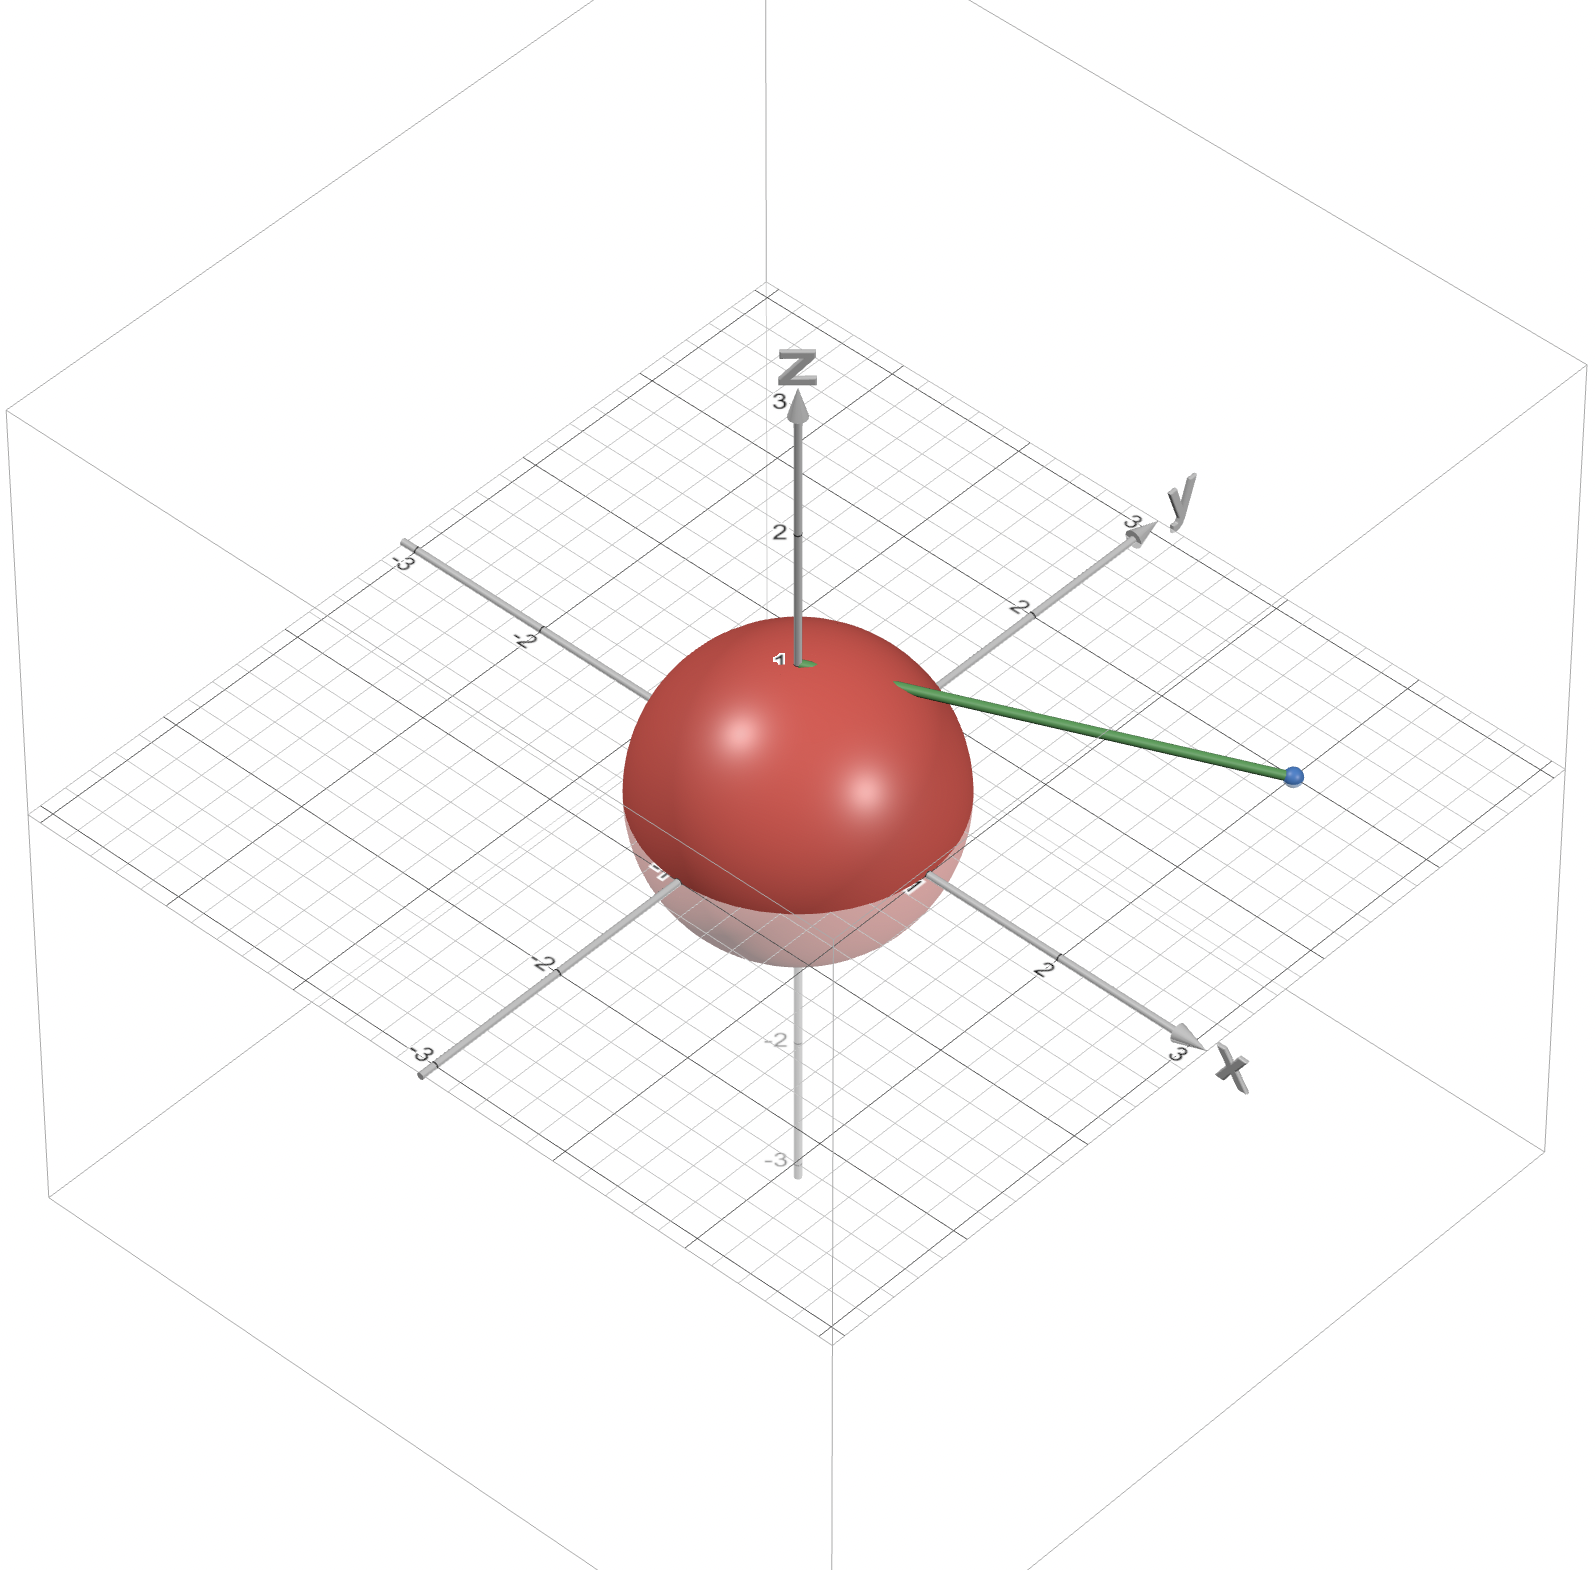
\includegraphics[width=.5\textwidth]{cox-little-oshea/ch1/assets/sec1-3-ex6a.png}
     \caption{Line between $(u,v,0)$ and $(0,0,1)$ for $u=v=2$ and the unit sphere.}
     \label{fig:sec1-3-ex8a}
    \end{figure}
    Remark: This appears on Brannan, Espen and Gray as the Stereographic projection.
    \item We know that the equation of a parametrised line in 3D is given by $r(t)=(x_0,y_0,z_0)+t(a,b,c)$, where $(a,b,c)$ are the slopes of the line. We can find the slopes, given two points, by simply subtracting one point from the other. We then have, $a=u, b=v$ and $c=-1$ then $r(t)=(0,0,1)+t(u,v,-1)=(tu,tv,1-t)$, as desired.
    \item We have 
    \begin{align*}
        &u^2t^2 + v^2t^2 + (1-t)^2 = 1 &&\iff\\
        &u^2t^2 + v^2t^2 + 1 - 2t + t^2 = 1 &&\iff\\
        &t^2(u^2 + v^2 + 1) - 2t = 0 &&\iff\\
        &t(u^2 + v^2 + 1) - 2 = 0 &&\iff\\
        &t = \frac{2}{u^2 + v^2 + 1}.
    \end{align*}
    Replacing $t$ in the above parametric equations of the line we obtain the desired result.
\end{enumerate}
\end{proof}

\begin{exercise}{7}
    Adapt the argument of the previous exercise to parametrize the ``sphere'' $x_1^2 + ... + x_n^2 = 1$ in $n$-dimensional affine space.
\end{exercise}
\begin{proof}
    Given a point $(u_1,...,u_{n-1},0)$. We draw the line to the ``north pole'' $(0,0,...,0,1)$ of the sphere and let $(x_1,...,x_n)$ be the other point where the line hits the sphere. The parametrization of said line is
    $$x_1 = tu_1,~....,~x_{n-1} = tu_{n-1},~x_n = 1 - t.$$
    We want to find $t$. Plugging this in, we get
    \begin{eqnarray*}
        1
        & = & x_1^2 + ... + x_n^2\\
        & = & (tu_1)^2 + ... + (tu_{n-1})^2 + (1-t)^2\\
        & = & t^2 (u_1^2 + ... + u_{n-1})^2 + 1 - 2t + t^2.
    \end{eqnarray*}
    We get
    $$t^2 (u_1^2 + ... + u_{n-1}^2 + 1) - 2t = 0.$$
    Thus, we see that $t=0$ (which is the north pole), or
    $$t = \frac{2}{u_1^2 + ... + u_{n-1}^2 + 1}.$$
    We get
    $$(x_1,...,x_n) = \frac{(2u_1, ..., 2 u_{n-1}, u_1^2 + ... + u_{n-1}^2 -1)}{u_1^2 + ... + u_{n-1}^2 + 1}.$$
    This is a parametrization of the $n-1$-sphere.
\end{proof}

\begin{exercise}{8}
Consider the curve defined by $y^2=cx^2-x^3$, where $c$ is some constant. Here is a picture of the curve when $c>0$:
\begin{figure}[H]
     \centering
     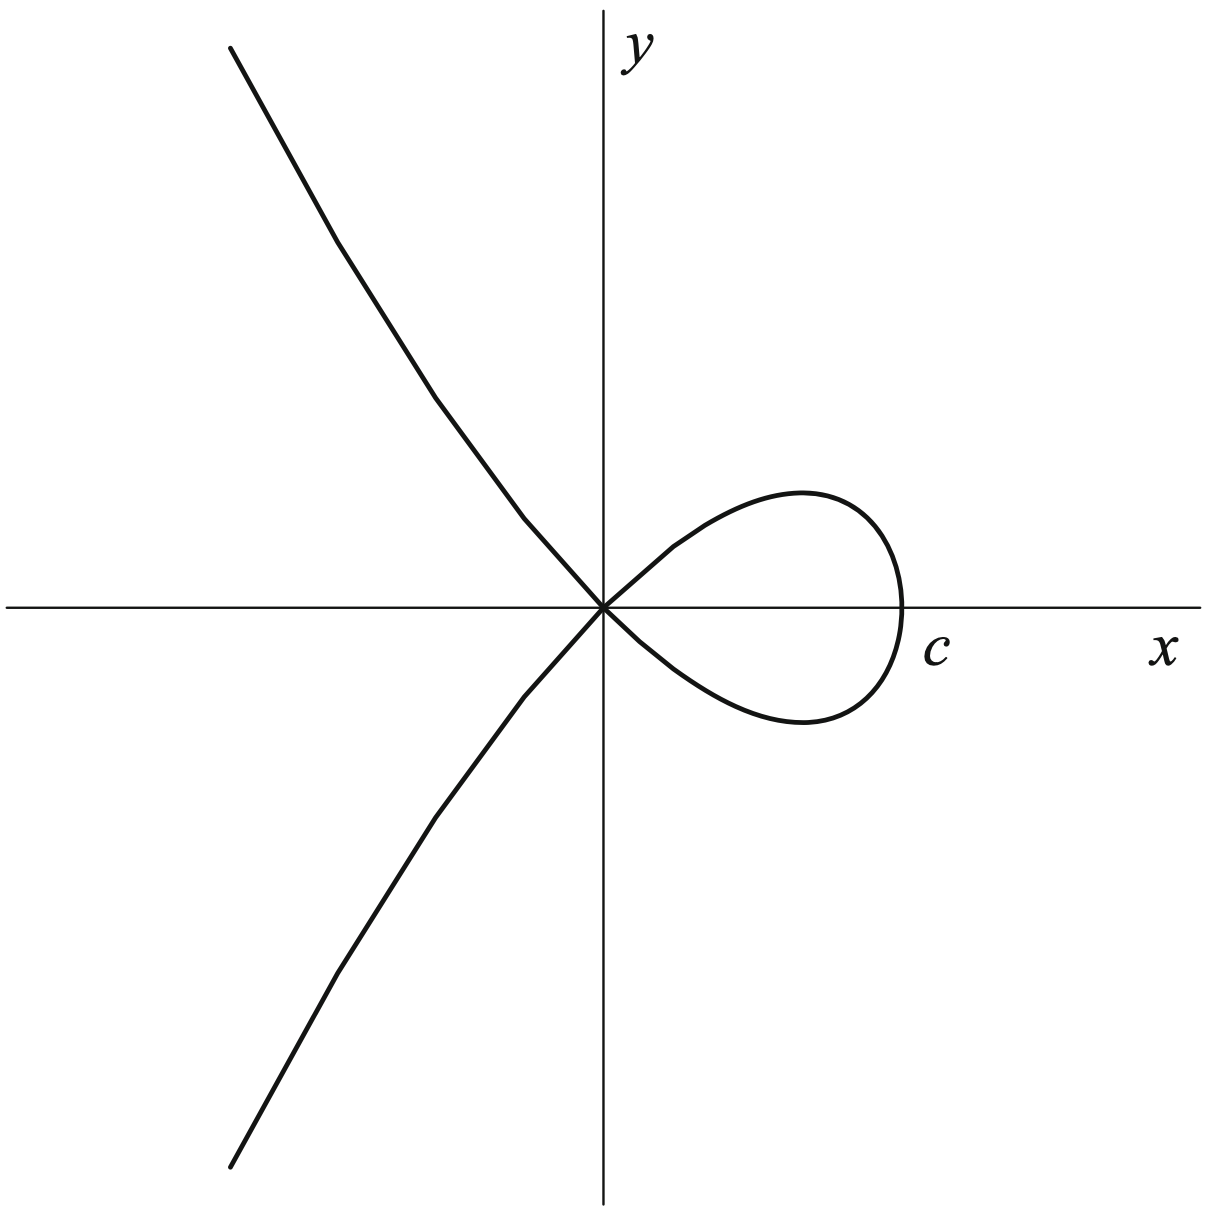
\includegraphics[width=.5\textwidth]{cox-little-oshea/ch1/assets/sec1-3-ex8.png}
     \label{fig:sec1-2-ex8}
\end{figure}
Our goal is to parametrise this curve.
\begin{enumerate}
    \item Show that a line will meet this curve at either 0, 1, 2, or 3 points. Illustrate your answer with a picture. Hint: let the equation of the line be either $x=a$ or $y=mx+b$.
    \item Show that a nonvertical line through the origin meets the curve at exactly one other point when $m^2\neq c$. Draw a picture to illustrate this, and see if you can come up with an intuitive explanation as to why this happens.
    \item Now draw the vertical line $x=1$. Given a point $(1,t)$ on this line, draw the line connecting $(1,t)$ to the origin. This will intersect the curve in a point $(x,y)$. Draw a picture to illustrate this, and argue geometrically that this gives a parametrisation of the entire curve.
    \item Show that the geometric description from part (3) leads to the parametrisation $x=c-t^2, y=t(c-t^2)$. 
\end{enumerate}
\end{exercise}
\begin{proof}
\begin{enumerate}
    \item Using the hint, consider the following two cases:

    Case 1. The line is vertical, with equation $x=a$. Then we have
    \begin{align*}
        y^2 =& ca^2-a^3\\
        =& a^2(c-a)\implies\\
        y =& a\sqrt{c-a}.
    \end{align*}
    We then have two extra cases. Case 1a: If $c-a\geq0$, then the line intersects the curve in the following two points $y=\pm a\sqrt{c-a}$, covering the 2 intersection case. Case 1b: If $c-a<0$, then the line does not intersect the curve, covering the 0 case.

    Case 2. The line is given by the following function $y=mx+b$. We have
    \begin{align*}
        &(mx+b)^2 = cx^2 -x^3 &&\implies\\
        &m^2x^2+2mbx+b^2 = cx^2-x^3 &&\implies\\
        &x^3+(m^2-c)x^2+2mbx+b^2 = 0 &&\text{(*)},
    \end{align*}
    which can have either 1 or 3 real roots (because complex roots come in pairs, covering the 1 or 3 intersection case.

    Cases 1a, 1b and 2 tell us that the lines can meet in 0, 1, 2 or 3 points.
    \item If $m^2\neq c$, and $b=0$ (because the line goes through the origin, we have that (*) is: $x^3+(m^2-c)x^2 = x^2(x+m^2-c)=0$, so that the roots of such polynomial are 0 and $x=c-m^2$. 
    
    My intuition of why this happens is that as we saw on (*), and replacing $b=0$, we must have 3 real roots, 0 being repeated. Hence, we are only left with $x+m^2-c=0$ which is a single intersection between the curves.
    \begin{figure}[H]
         \centering
         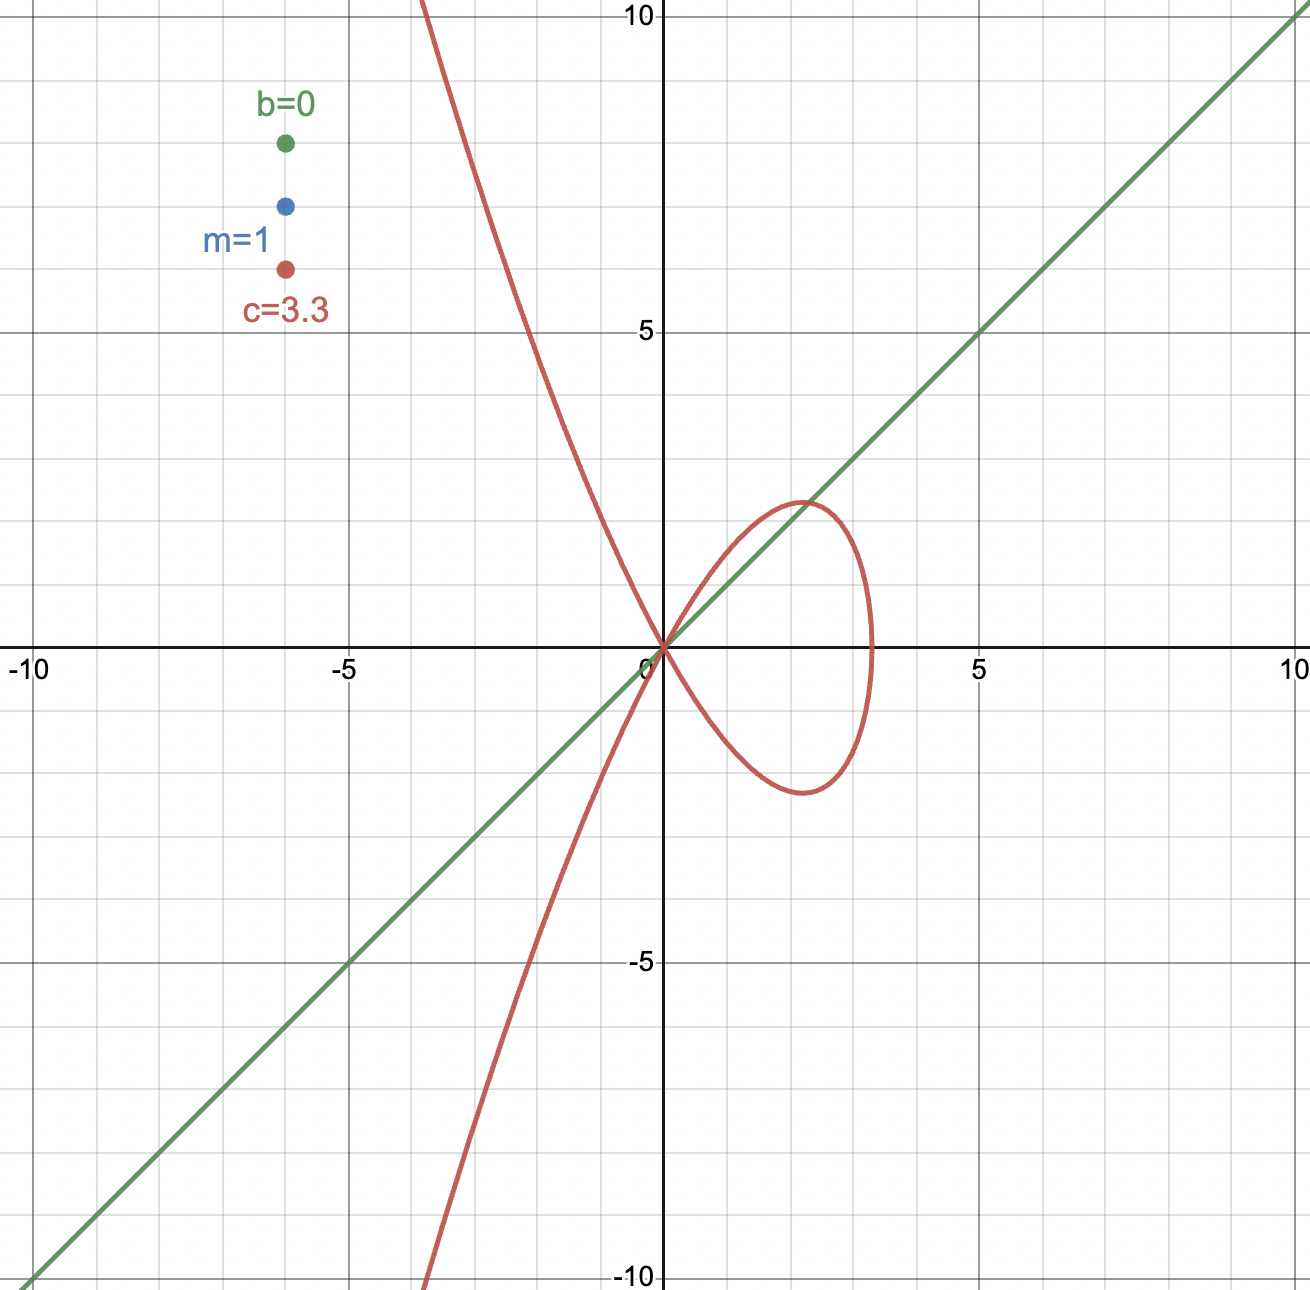
\includegraphics[width=.5\textwidth]{cox-little-oshea/ch1/assets/sec1-3-ex8-sol2.png}
         \label{fig:sec1-2-ex8-sol2}
    \end{figure}

    \item We just argued in the previous exercise that a line that goes through the origin meets the curve at a single point. Geometrically, this is a parametrisation of the whole curve because the line through $(1,t)$ and the origin will have any slope we want, with functional form $y=mx$. Since the intersection between this line and $y$ is given by (*) (with $b=0$), we cover all values of $y$. To see this, just choose $(1,t)$ so that $m$ gives the desired value of $y$ whenever we replace $x=c-m^2$ in the original function of the equation.
    \begin{figure}[H]
         \centering
         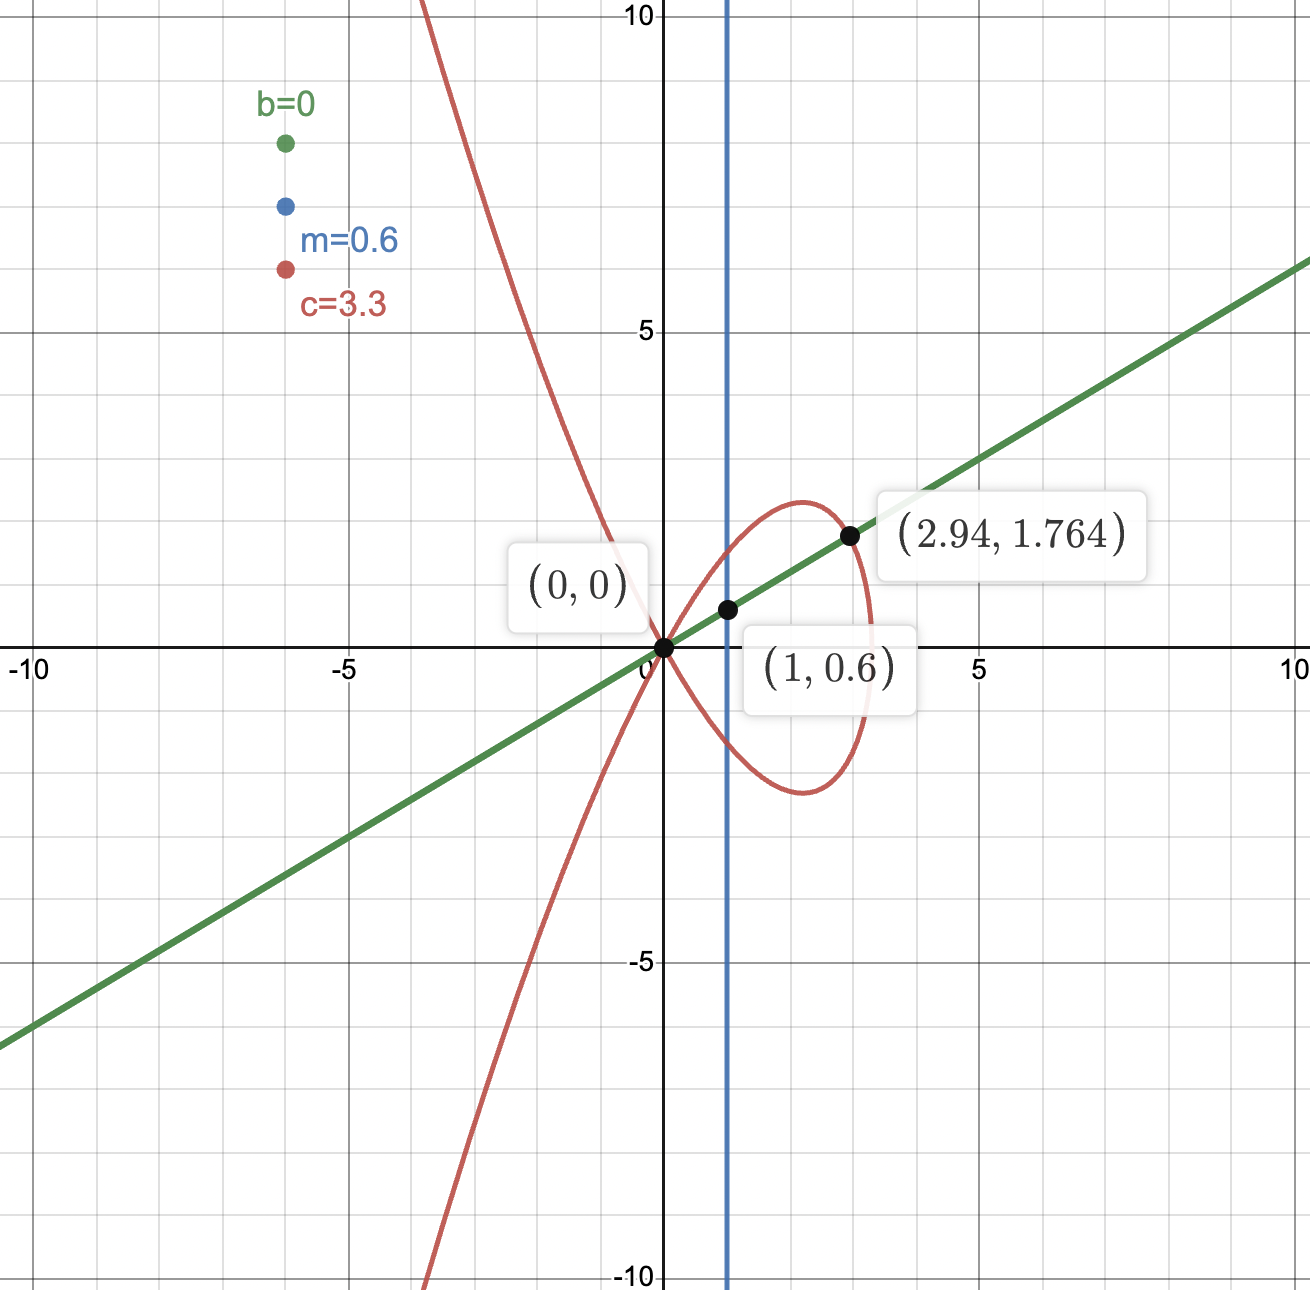
\includegraphics[width=.5\textwidth]{cox-little-oshea/ch1/assets/sec1-3-ex8-sol3.png}
         \label{fig:sec1-2-ex8-sol3}
    \end{figure}
    \item We just argued before about $x=c-m^2$, which translates to $x=c-t^2$ given that we are using the vertical curve $x=1$. To see the parametrisation for $y$, we substitute as we intuitively argued above: $y=\sqrt{c(c-t^2)^2-(c-t^2)^3}=\sqrt{t^2(c-t^2)^2}=t(c-t^2)$, as required.
\end{enumerate}
\end{proof}

\begin{exercise}{9}
The strophoid is a curve that was studied by various mathematicians, including Isaac Barrow ($1630-1677$), Jean Bernoulli ($1667-1748$), and Maria Agnesi ($1718-1799$).A trigonometric parametrization is given by
\begin{eqnarray*}
    x & = & a\sin(t),\\
    y & = & a\tan(t)( 1 + \sin(t) )
\end{eqnarray*}
where $a$ is a constant.
    \begin{enumerate}
        \item Find the equation in $x$ and $y$ that describes the strophoid.
        \item Find an algebraic parametrization of the strophoid.
    \end{enumerate}
\end{exercise}
\begin{proof}
    \begin{enumerate}
        \item We get that
        $$y\cos t = a\sin t (1 + \sin t),$$
        and thus by squaring
        $$y^2 \cos^2 t = a^2 \sin^2 t ( 1  + \sin t)^2,$$
        and thus
        $$a^2 y^2 (1 - \sin^2 t) = a^2 \sin^2 t ( a + a\sin t)^2.$$
        Replacing $x=a\sin t$, we get
        $$y^2 (a^2 - x^2) = x^2 (a + x)^2$$
        and thus
        $$y^2 (a-x)(a+x) = x^2 (a+x)^2.$$
        Note however that $x+a = a(1 + \sin(t))$ only gives us zero when $t = -\pi/2 + 2k\pi$. But in those points, $y$ is undefined. So the curve never hits the line $x+a = 0$, which we can therefore cancel:
        $$y^2 (a-x) = x^2 (a+x).$$
        Assume first that $a=0$, then we get $-y^2 x = x^3$. If $x\neq 0$, then $-y^2 = x^2$, which cannot happen. So only $(0,0)$ is in the graph, and clearly there is some $t$ such that $x=0\sin(t)$ and $y = a\tan(t) (1 + \sin(t))$.\\

        Next, assume that $a>0$. Then if $x\geq a$, we see that $a-x\leq 0$ and $a+x>0$, which contradicts the equation $y^2 (a-x) = x^2 (a+x)$. Similarly, if $x<-a$, then $a-x>0$ and $a+x<0$, contradicting the equation again. Thus, we see that $-a\leq x<a$. We see that there is some $t\in (-3\pi/2,\pi/2)$ such that $a\sin(t) = x$. Note that if $t=-\pi/2$, then $x=-a$ and thus $y=0$. The equation $y = a\tan(t) (1+\sin(t))$ kind of makes sense in this case as well since you multiply by $0$. In the case $t\neq -\pi/2$, we see that
        \begin{eqnarray*}
            y^2
            & = & x^2\frac{a+x}{a-x}\\
            & = & a^2 \sin^2 t \frac{a + a\sin t}{a - a\sin(t)}\\
            & = & a^2 \sin^2 t \frac{1 + \sin(t)}{1 - \sin(t)}\\
            & = & a^2 \sin^2 t \frac{(1 + \sin(t))^2}{1 - \sin^2(t)}\\
            & = & a^2 \tan^2(t) (1 + \sin(t))^2.
        \end{eqnarray*}
        Thus, $y = a|\tan(t)|(1 + \sin(t))$. Replacing $t$ by $\pi - t$ if necessary, we keep the equation $x = a\sin(t)$, but we can always assume $y = a\tan(t)(1+\sin(t))$ as well.\\

        The case $a<0$ is just the reflection of the case $-a>0$ over the $y$-axis and thus is handled similarly. In each case, we see that the curve is described by the equation
        $$y^2 (a-x) = x^2 (a+x).$$    

        \item Let us consider the line $y=tx$ for a parameter $t$. We get
        \begin{eqnarray*}
            0 
            & = & y^2 (a-x) - x^2 (a+x)\\
            & = & t^2 x^2 (a-x) - x^2 (a+x)\\
            & = & x^2 ( t^2(a-x) - (a+x))\\
            & = & x^2 (  t^2 a - t^2 x - a - x)\\
            & = & x^2 (  (t^2 - 1)a - (1+t^2) x).
        \end{eqnarray*}
        We see that $x=0$ or
        $$x = \frac{t^2 - 1}{1 + t^2}.$$
        Then,
        $$y = tx = \frac{t^3 - t}{1 + t^2}.$$
        It is clear by this construction that every point on the strophoid has a corresponding $t$.
    \end{enumerate}
\end{proof}

\begin{exercise}{10}
    Around $180$ B.C.E., Diocles wrote the book \emph{On Burning-Glasses}. One of the curves he considered was the \emph{cissoid} and he used it to solve the problem of the duplication of the cube. The cissoid has the equation $y^2 (a+x) = (a-x)^3$, where $a$ is a constant. 
    \begin{enumerate}
        \item Find an algebraic parametrization of the cissoid.
        \item Diocles described the cissoid using the following geometric construction. Given a circle of radius $a$ (which we will take as centered at the origin), pick $x$ between $a$ and $-a$, and draw the line $L$ connecting $(a,0)$ to the point $P = (-x,\sqrt{a^2 - x^2})$ on the circle. This determines a point $Q = (x,y)$ on $L$. Prove that the cissoid is the locus of all such points $Q$.
         \item The duplication of the cube is the classical Greek problem of trying to construct $\sqrt[3]{2}$ using ruler and compass. It is known that this is impossible given just a ruler and compass. Diocles showed that if in addition, you allow the use of the cissoid, then one can construct $\sqrt[3]{2}$. Here is how it works. Draw the line connecting $(-a,0)$ to $(0,a/2)$. This line will meet the cissoid at a point $(x,y)$. Then prove that
         $$2 = \left(\frac{a-x}{y}\right)^3,$$
         which shows how to construct $\sqrt[3]{2}$ using ruler, compass, and cissoid.
    \end{enumerate}
\end{exercise}
\begin{proof}
\begin{enumerate}
    \item A line through the point $(a,0)$ has the equation $y = t(x-a)$. Thus, we get for the cissoid that
    \begin{eqnarray*}
        0
        & = & y^2 (a+x) - (a-x)^3\\
        & = & t^2 (a-x)^2 (a+x) - (a-x)^3\\
        & = & (a-x)^2 ( t^2 (a+x) - (a-x))\\
        & = & (a-x)^2 ( t^2 a + t^2 x - a + x)\\
        & = & (a-x)^2 ( (1+t^2)x - (1 - t^2)a).
    \end{eqnarray*}
    Thus, we see that either $x=a$ or
    $$x = \frac{1-t^2}{1+t^2}a,$$
    which also yields $x=a$ if $t=0$. Then,
    $$y = \frac{-2t^3}{1+t^2}a.$$
    \item The line through $(a,0)$ and $P$ has equation:
    $$Y = \frac{\sqrt{a^2 - x^2}}{-x-a}(X-a).$$
    Plugging in $X = x$, we get
    \begin{eqnarray*}
        y^2
        & = & \left(\frac{\sqrt{a^2 - x^2}}{-x-a}(x-a)\right)\\
        & = & \frac{a^2 - x^2}{(x+a)^2}(x-a)^2\\
        & = & \frac{(a-x)(a+x)}{(x+a)^2}(x-a)^2\\
        & = & \frac{(a-x)}{x+a}(a-x)^2\\
        & = & \frac{(a-x)^3}{x+a},
    \end{eqnarray*}
    giving the cissoid equation immediately.\\
    Conversely, assume that $y^2 (a+x) = (a-x)^3$. Assume that $a>0$. If $x>a$, then $a+x>0$ and $a-x\leq 0$, a contradiction. Likewise, if $x\leq -a$, then $x+a\leq 0$ and $a-x>0$, a contradiction too. We obtain that $x\in (-a,a]$. In particular, the following does not give a division by zero:
    \begin{eqnarray*}
        y^2
        & = & \frac{(a-x)^3}{x+a}\\
        & = & \frac{(a-x)}{x+a}(a-x)^2\\
        & = & \frac{(a-x)(a+x)}{(x+a)^2}(x-a)^2\\
        & = & \frac{a^2 - x^2}{(x+a)^2}(x-a)^2.    
    \end{eqnarray*}
    Since $a\in (-a,a]$, we know that $(x+a)/(x-a)\geq 0$, thus,
    $$y = \frac{\sqrt{a^2 - x^2}}{-x-a}(x-a).$$
    Thus this is the point on the line
    $$Y = \frac{\sqrt{a^2 - x^2}}{-x-a}(X-a)$$
    with $x$-coordinate $x$. We get that thus that the point $(x,y)$ is obtained by the construction of Diocles.
    \item The line connecting $(-a,0)$ and $(0,a/2)$ is given by
    $$y = \frac{a/2}{a}(x+a) = \frac{1}{2}(x+a).$$
    Plugging $x+a = 2y$ into the equation of the cissoid, we get
    \begin{eqnarray*}
        0
        & = & y^2 (a+x) - (a-x)^3\\
        & = & 2y^3 - (a-x)^3,
    \end{eqnarray*}
    from which we clearly get that
    $$2 = \frac{(a-x)^3}{y^3}.$$
\end{enumerate}
\end{proof}

\begin{exercise}{11}
In this problem, we will derive the parametrisation
\begin{align*}
    x = t(u^2-t^2),\,\, y = u,\,\, z = u^2-t^2
\end{align*}
of the surface $x^2-y^2z^2+z^3=0$ considered in the text.
\begin{enumerate}
    \item Adapt the formulas in part (4) of exercise 8 to show that the curve $x^2 = cz^2-z^3$ is parametrized by 
    \begin{align*}
        z=c-t^2,\,\, x=t(c-t^2).
    \end{align*}
    \item Now replace the c in part (1) by $y^2$, and explain how this leads to the above parametrisation of $x^2-y^2z^2+z^3=0$.
    \item Explain why this parametrisation covers the entire surface $\bV(x^2-y^2z^2+z^3$. Hint: See part (3) of exercise 8.
\end{enumerate}
\end{exercise}
\begin{proof}
\begin{enumerate}
    \item These are exactly the same formulas as in part (4) of 8, where $x=y$ and $z=x$. 
    \item After replacing $c=y^2$, we have $x^2=y^2z^2-z^3$, which is exactly the parametrisation we want.
    \item As argued on the two previous solutions, the formulas here presented are the same as in Exercise 8 where $x=y$ and $z=x$. Furthermore, instead of having $c$ as a parameter as in Exercise 8, we introduce a new variable to take on that value, namely $y^2=c$. Since the reasons of why the parametrisation in Exercise 8 did not depend on the value of $c$, then we simply introduce a new variable, $y$, and parameter, $u$, without affecting the fact that the entire surface is covered by the parametrisation.
\end{enumerate}
\end{proof}

\begin{exercise}{12}
Consider the variety $V = \bV(y-x^2,z-x^4)\subseteq\mathbb{R}^3$.
\begin{enumerate}
    \item Draw a picture of $V$.
    \item Parametrize $V$ in a way similar to what we did with the twisted cubic.
    \item Parametrize the tangent surface of $V$.
\end{enumerate}
\end{exercise}
\begin{proof}
    \begin{enumerate}
        \item We get
        \begin{figure}[H]
            \centering
            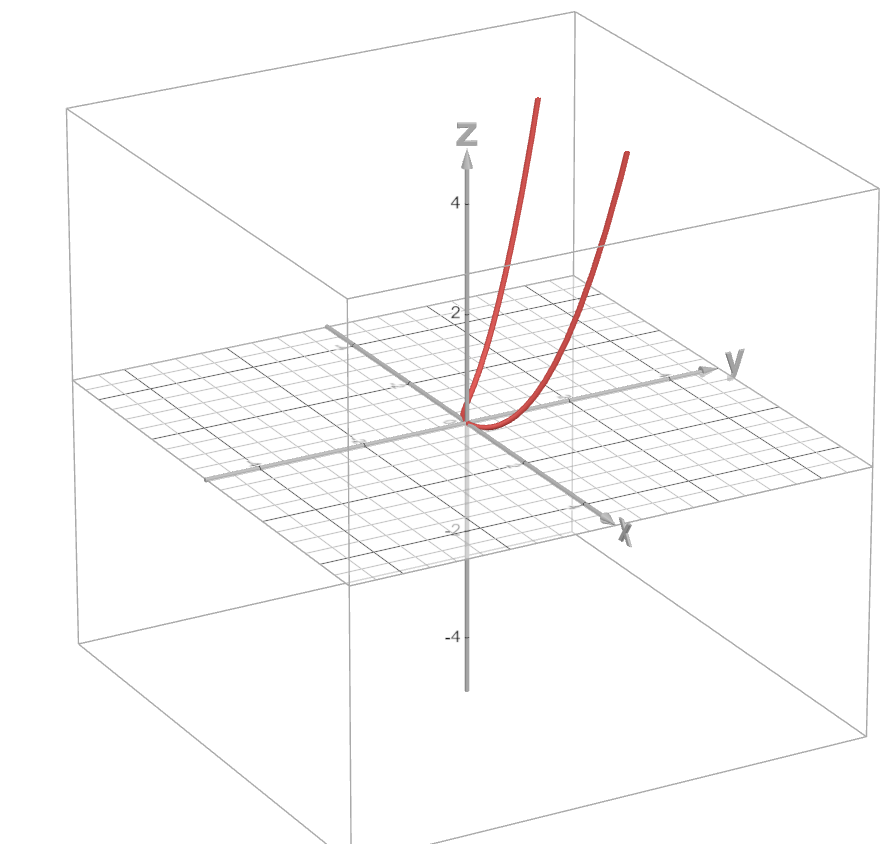
\includegraphics[width=0.5\linewidth]{cox-little-oshea/ch1/assets/sec1-3-ex12.png}
            \caption{Graph of the variety $V = \bV(y-x^2,z-x^4)$}
            \label{fig:sec1-3-ex12}
        \end{figure}
        \item It is clear the parametrization becomes
        \begin{eqnarray*}
            x & = & t,\\
            y & = & t^2,\\
            z & = & t^4.
        \end{eqnarray*}
        Thus, $\mathbf{r}(t)= (t, t^2, t^4)$.
        \item Notice that the tangent vector at the point given by $\mathbf{r}(t)$ is 
        $$\mathbf{r}'(t) = (1, 2t, 4t^3).$$
        It follows that the tangent line is parametrized by
        $$\mathbf{r}(t) + u\mathbf{r}'(t) = (t + u, t^2 + 2tu, t^4 + 4t^3 u).$$
        Thus, we get the parametrization
        \begin{eqnarray*}
            x & = & t+u\\
            y & = & t^2 + 2tu\\
            z & = & t^4 + 4t^3 u.
        \end{eqnarray*}
    \end{enumerate}
\end{proof}

\begin{exercise}{13}
The general problem of finding the equation of a parametrized surface will be studied in Chapters $2$ and $3$. However, when the surface is a plane, methods from calculus or linear algebra can be used. For example, consider the plane in $\mathbb{R}^3$ parametrized by
\begin{eqnarray*}
    x & = & 1 + u - v,\\
    y & = & u + 2v,\\
    z & = & -1 - u + v.
\end{eqnarray*}
Find the equation of the plane determined this way.
\end{exercise}
\begin{proof}
    Let the equation of the plane by $ax+by+cz = d$. Hence,
    \begin{eqnarray*}
        d
        & = & ax+by+cz\\
        & = & a(1+u-v) + b(u + 2v) + c(-1 - u + v)\\
        & = & (a-c) + u(a + b - c) + v(-a + 2b + c).
    \end{eqnarray*}
    We get a polynomial in $u$ and $v$ which has to be zero everywhere:
    $$u(a + b - c) + v(-a + 2b + c) + (a-c-d) = 0.$$
    We then know that the coefficients must be zero, yielding the equations
    \begin{eqnarray*}
        a + b - c & = & 0\\
        -a + 2b + c & = & 0\\
        a -c - d = 0.
    \end{eqnarray*}
    Adding the first two equations gives us $b=0$. We then get the following equations
    \begin{eqnarray*}
        a - c & = & 0\\
        a - c - d & = & 0,
    \end{eqnarray*}
    Giving us $a=c$ and $d = a - c = 0$. We get that
    $$x + z = 0$$
    is the equation of the plane.
\end{proof}

\begin{exercise}{14}
This problem deals with convex sets and will be used in the next exercise to show that a B\'ezier cubic lies within its control polygon. A subset $C\subseteq \mathbb{R}^2$ is convex if for all $P,Q\in C$, the line segment joining $P$ to $Q$ also lies in $C$.
\begin{enumerate}
    \item If $P = \left(\begin{array}{c} x\\ y\end{array}\right)$ and $Q = \left(\begin{array}{c} z\\ w\end{array}\right)$ lie in a convex set $C$, then show that
    $$t\left(\begin{array}{c} x\\ y\end{array}\right) + (1-t)\left(\begin{array}{c} z\\ w\end{array}\right)\in C$$
    when $0\leq t\leq 1$.
    \item If $P_i = \left(\begin{array}{c} x_i\\ y_i\end{array}\right)$ lies in a convex set $C$ for $1\leq i \leq n$, then show that
    $$\sum_{i=1}^n t_i \left(\begin{array}{c} x_i\\ y_i\end{array}\right)\in C$$
    wherever $t_1,...,t_n$ are nonnegative numbers such that $\sum_{i=1}^n t_i = 1$. 
\end{enumerate}
\end{exercise}
\begin{proof}
    \begin{enumerate}
        \item This is easy since the formula given is exactly a parametrization of the line segment through $P$ and $Q$.
        \item The statement is trivial for $n=1$. Assume the statement is true for $n$, then take nonnegative numbers $t_1,...,t_{n+1}$ with $\sum_{i=1}^{n+1} t_i = 1$. Then let 
        $$s_i = \frac{t_i}{\sum_{k=1}^n t_k}.$$
        We see that $\sum_{i=1}^n s_i = 1$, and thus
        $$\sum_{i=1}^n s_i \left(\begin{array}{c} x_i\\ y_i\end{array}\right)\in C.$$
        By part (a), 
    $$(1 - t_{n+1})\sum_{i=1}^n s_i \left(\begin{array}{c} x_i\\ y_i\end{array}\right) + t_{n+1}\left(\begin{array}{c} x_{n+1}\\ y_{n+1}\end{array}\right)\in C.$$
    But,
    \begin{eqnarray*}
        (1 - t_{n+1})\sum_{i=1}^n s_i \left(\begin{array}{c} x_i\\ y_i\end{array}\right) + t_{n+1}\left(\begin{array}{c} x_{n+1}\\ y_{n+1}\end{array}\right)
        & = & \left(\sum_{i=1}^{n+1} t_i - t_{n+1}\right)\sum_{i=1}^n s_i \left(\begin{array}{c} x_i\\ y_i\end{array}\right) + t_{n+1}\left(\begin{array}{c} x_{n+1}\\ y_{n+1}\end{array}\right)\\
        & = & \left(\sum_{i=1}^n t_i\right)\sum_{i=1}^n s_i \left(\begin{array}{c} x_i\\ y_i\end{array}\right) + t_{n+1}\left(\begin{array}{c} x_{n+1}\\ y_{n+1}\end{array}\right)\\
        & = & \left(\sum_{i=1}^n t_i\right)\sum_{i=1}^n \frac{t_i}{\sum_{k=1}^n t_k} \left(\begin{array}{c} x_i\\ y_i\end{array}\right) + t_{n+1}\left(\begin{array}{c} x_{n+1}\\ y_{n+1}\end{array}\right)\\
        & = & \sum_{i=1}^n t_i \left(\begin{array}{c} x_i\\ y_i\end{array}\right) + t_{n+1}\left(\begin{array}{c} x_{n+1}\\ y_{n+1}\end{array}\right)\\
        & = & \sum_{i=1}^{n+1} t_i \left(\begin{array}{c} x_i\\ y_i\end{array}\right).
    \end{eqnarray*}
    This proves the induction.
    \end{enumerate}
\end{proof}

\begin{exercise}{15}
    Let a B\'ezier cubic be given by
    \begin{eqnarray*}
        x & = & (1-t)^3 x_0 + 3t(1-t)^2 x_1 + 3t^2 (1-t) x_2 + t^3 x_3,\\
        x & = & (1-t)^3 y_0 + 3t(1-t)^2 y_1 + 3t^2 (1-t) y_2 + t^3 y_3.        
    \end{eqnarray*}
    
    \begin{enumerate}
        \item Show that the above equations can be written in vector form
        \begin{align*}
            \parens{
            \begin{array}{c} 
                x\\ 
                y
            \end{array}}
            = (1-t)^3 
            \parens{
            \begin{array}{c} 
                x_0\\ 
                y_0
            \end{array}} 
            + 3t(1-t)^2 
            \parens{
            \begin{array}{c} 
                x_1\\ 
                y_1
            \end{array}} 
            + 3t^2 (1-t) 
            \parens{
            \begin{array}{c} 
                x_2\\ 
                y_2
            \end{array}} 
            + t^3 
            \parens{
            \begin{array}{c} 
                x_3\\ 
                y_3
            \end{array}}.
        \end{align*}
        \item Use the previous exercise to show that a B\'{e}zier cubic always lies inside its control polygon.
    \end{enumerate}
\end{exercise}
\begin{proof}
    \begin{enumerate}
        \item This is trivial by looking at the equation in the two components. 
        \item We see that
        \begin{eqnarray*}
            (1-t)^3 + 3t(1-t)^2 + 3t^2 (1-t) + t^3
            & = & ( (1-t) + t)^3\\
            & = & 1^3\\
            & = & 1.
        \end{eqnarray*}
        Thus, since the sum of the coefficients is $1$, and the control polygon is by definition convex, we see that $(x,y)$ lies in the control polygon for all $t$.
    \end{enumerate}
\end{proof}

\begin{exercise}{16}
One disadvantage of B\'ezier cubics is that curves like circles and hyperbolas cannot be described exactly by cubics. In this exercise, we will discuss a method similar to example (4) for parametrizing conic sections.\\

A conic section is a curve in the plane defined by a second degree equation of the form $ax^2 + bxy + cy^2 + dx + ey = 0$. Conic sections include the familiar examples of circles, ellipses, parabolas, and hyperbolas. Now consider the curve parametrized by
\begin{eqnarray*}
    x & = & \frac{(1-t)^2 x_1 + 2t(1-t)wx_2 + t^2 x_3}{(1-t)^2 + 2t(1-t)w + t^2},\\
    y & = & \frac{(1-t)^2 y_1 + 2t(1-t)wy_2 + t^2 y_3}{(1-t)^2 + 2t(1-t)w + t^2}    
\end{eqnarray*}
for $0\leq t\leq 1$. The constants $w,x_1,y_1,x_2,y_2,x_3,y_3$ are specified by the design engineer, and we will assume that $w\geq 0$. In Chapter $3$, we will show that these equations parametrize a conic section. The goal of this exercise is to give a geometric interpretation for the quantities $w,x_1,y_1,x_2,y_2,x_3,y_3$.
    \begin{enumerate}
        \item Show that our assumption $w\geq 0$ implies that the denominator in the above formulas never vanishes.
        \item Evaluate the above formulas at $t=0$ and $t=1$. This should tell you what $x_1$, $y_1$, $x_3$, $y_3$ mean.
        \item Now compute $(x'(0), y'(0))$ and $(x'(1), y'(1))$. Use this to show that $(x_2,y_2)$ is the intersection of the tangent lines at the start and end of the curve. Explain why $(x_1,y_1)$, $(x_2,y_2)$ and $(x_3,y_3)$ are called the control points of the curve.
        \item Define the control polygon (it is actually a triangle in this case), and prove that the curve defined by the above equations always lies in its control polygon. This gives the following picture:\\
        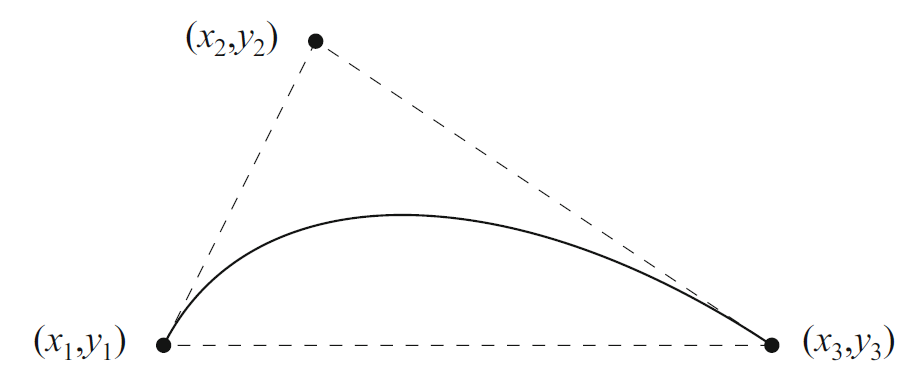
\includegraphics[width=0.8\linewidth]{cox-little-oshea/ch1/assets/sec1-3-ex16.png}
        It remains to explain the constant $w$, which is called the shape factor. A hint should come from the answer to part (c), for note that $w$ appears in the formulas for the tangent vectors when $t=0$ and $1$. So $w$ somehow controls the ``velocity,'' and a larger $w$ should force the curve closer to $(x_2,y_2)$. In the last two parts of the problem, we will determine exactly what $w$ does.
        \item Prove that
        $$\left(\begin{array}{c}x\left(\frac{1}{2}\right)\\ y\left(\frac{1}{2}\right)\end{array}\right) = \frac{1}{1+w}\left(\frac{1}{2}\left(\begin{array}{c}x_1\\ y_1\end{array}\right) + \frac{1}{2}\left(\begin{array}{c}x_3\\ y_3\end{array}\right) \right) + \frac{w}{1+w}\left(\begin{array}{c}x_2\\ y_2\end{array}\right).$$
        Use this formula to show that $\left(x\left(\frac{1}{2}\right),y\left(\frac{1}{2}\right)\right)$ lies on the line segment connecting $(x_2,y_2)$ to the midpoint between $(x_1,y_1)$ and $(x_3,y_3)$.\\
        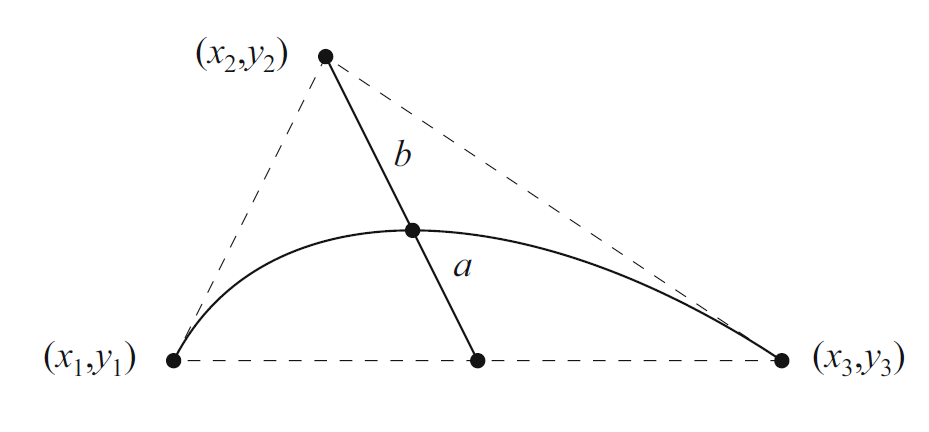
\includegraphics[width=0.8\linewidth]{cox-little-oshea/ch1/assets/sec1-3-ex16a.png}
        \item Notice that $\left(x\left(\frac{1}{2}\right), y\left(\frac{1}{2}\right)\right)$ divides this line segment into two pieces, say of length $a$ and $b$ as indicated in the above picture. Then prove that
        $$w = \frac{a}{b},$$
        so that $w$ tells us exactly where the curve crosses this line segment.
    \end{enumerate}
\end{exercise}
\begin{proof}
    \begin{enumerate}
        \item Since $w\geq 0$, we see that
        $$(1-t)^2 + 2t(1-t)w + t^2\geq (1-t)^2 + t^2 > 0.$$
        \item As $t=0$, we get
\begin{align*}
    x & = \frac{(1-t)^2 x_1 + 2t(1-t)wx_2 + t^2 x_3}{(1-t)^2 + 2t(1-t)w + t^2} & = x_1,\\
    y & = \frac{(1-t)^2 y_1 + 2t(1-t)wy_2 + t^2 y_3}{(1-t)^2 + 2t(1-t)w + t^2} & = y_1.   
\end{align*}        
We get for $t=1$, that
\begin{align*}
    x & = \frac{(1-t)^2 x_1 + 2t(1-t)wx_2 + t^2 x_3}{(1-t)^2 + 2t(1-t)w + t^2} & = x_3,\\
    y & = \frac{(1-t)^2 y_1 + 2t(1-t)wy_2 + t^2 y_3}{(1-t)^2 + 2t(1-t)w + t^2} & = y_3.   
\end{align*}     
So we see that $(x_1,y_1)$ and $(x_3, y_3)$ are the begin and endpoints of the segment.
\item We see that 
$$x'(t) = \frac{2w(-x_1(t-1)^2 + 2x_2t + x_2 + x_3t^2) + 2(t-1)t(x_1 - x_3)}{(1 - 2(t-1)t(w-1))^2}.$$
We get,
$$x'(0) = 2w(x_2 - x_1),~~y'(0) = 2w(x_3 - x_2).$$
Similarly,
$$y'(0) = 2w(y_2 - y_1),~~y'(0) = 2w(y_3 - y_2).$$
The tangent line through $(x_1, y_1)$, is given by
$$f(t) = (x(0),y(0)) + t(x'(0),y'(0)) = (x_1 + 2wt (x_2 - x_1), y_1 + 2wt(y_2 - y_1)).$$
Putting $t= \frac{1}{2w}$, we get that $(x_2,y_2)$ is on this tangent line. Similarly, it is on the tangent line $g(t) = (x(1),y(1)) + t(x'(1),y'(1))$. This establishes that $(x_2,y_2)$ is on the intersection of the two tangent lines. We say that $(x_1,y_1)$, $(x_2, y_2)$ and $(x_3,y_3)$ are called the control points since they control completely geometrically what the curve looks like.
\item We can write
\begin{eqnarray*}
    \left(\begin{array}{c} x\\ y \end{array}\right) 
    & = &\frac{(1-t)^2}{(1-t)^2 + 2t(1-t)w + t^2}\left(\begin{array}{c} x_1\\ y_1 \end{array}\right)\\
    & & +\frac{2t(1-t)w}{(1-t)^2 + 2t(1-t)w + t^2}\left(\begin{array}{c} x_2\\ y_2  \end{array}\right)\\
    & & + \frac{t^2}{(1-t)^2 + 2t(1-t)w + t^2}\left(\begin{array}{c} x_1\\ y_1 \end{array}\right).
\end{eqnarray*}
Note that each of the three coefficients is in $[0,1]$, and they clearly add up to $1$. Thus since $(x,y)$ is a convex combination of $(x_1,y_1)$, $(x_2,y_2)$ and $(x_3,y_3)$, we see that $(x,y)$ is in the control polygon.
\item We see that
\begin{eqnarray*}
   x\left(\frac{1}{2}\right)
   & = & \frac{\left(1-\frac{1}{2}\right)^2 x_1 + 2\frac{1}{2}\left(1-\frac{1}{2}\right)wx_2 + \left(\frac{1}{2}\right)^2 x_3}{\left(1-\frac{1}{2}\right)^2 + 2\frac{1}{2}\left(1-\frac{1}{2}\right)w + \left(\frac{1}{2}\right)^2}\\
   & = & \frac{\left(\frac{1}{2}\right)^2 x_1 + 2\frac{1}{2}\left(\frac{1}{2}\right)wx_2 + \left(\frac{1}{2}\right)^2 x_3}{\left(\frac{1}{2}\right)^2 + 2\frac{1}{2}\left(\frac{1}{2}\right)w + \left(\frac{1}{2}\right)^2}\\
   & = & \frac{\frac{1}{4} x_1 + 2\frac{1}{4}wx_2 + \frac{1}{4} x_3}{\frac{1}{4} + 2\frac{1}{4}w + \frac{1}{4}}\\
   & = & \frac{\frac{1}{4} x_1 + \frac{1}{2}wx_2 + \frac{1}{4} x_3}{\frac{1}{2} + \frac{1}{2}w}\\
   & = & \frac{\frac{1}{2} x_1 + wx_2 + \frac{1}{2} x_3}{1+w}\\
   & = & \frac{1}{2}\frac{x_1}{1+w} + \frac{w}{1+w}x_2 + \frac{1}{2}\frac{x_3}{1+w}\\
   & = & \frac{1}{1+w}\left(\frac{1}{2}x_1 + \frac{1}{2}x_3\right) + \frac{w}{1+w}x_3.
\end{eqnarray*}
A similar computation holds for $y\left(\frac{1}{2}\right)$.
    \item The midpoint between $(x_1,y_1)$ and $(x_3,y_3)$ has coordinates 
    $$\left(\begin{array}{c}x_{\text{mid}}\\ y_{\text{mid}}\end{array}\right) = \frac{1}{2}\left(\begin{array}{c}x_1\\ y_1\end{array}\right) + \frac{1}{2}\left(\begin{array}{c}x_3\\ y_3\end{array}\right).$$
    Thus,
    $$\left(\begin{array}{c}x\left(\frac{1}{2}\right)\\ y\left(\frac{1}{2}\right)\end{array}\right) = \frac{1}{1+w}\left(\begin{array}{c}x_{\text{mid}}\\ y_{\text{mid}}\end{array}\right) + \frac{w}{1+w}\left(\begin{array}{c}x_2\\ y_2\end{array}\right).$$
    By Exercise $14$ and choosing $t = \frac{1}{1+w}$, we then see that $\left(x\left(\frac{1}{2}\right),y\left(\frac{1}{2}\right)\right)$ is part of the line going through $(x_{\text{mid}},y_{\text{mid}})$ and $(x_2,y_2)$, as desired.
    \item Note that
    \begin{eqnarray*}
        \frac{a}{b}
        & = & \frac{\left\|\left(\begin{array}{c} x\left(\frac{1}{2}\right)\\ y\left(\frac{1}{2}\right)\end{array}\right) - \left(\begin{array}{c} x_{\text{mid}}\\ y_{\text{mid}}\end{array}\right)\right\|}{\left\|\left(\begin{array}{c} x\left(\frac{1}{2}\right)\\ y\left(\frac{1}{2}\right)\end{array}\right) - \left(\begin{array}{c} x_2\\ y_2\end{array}\right)\right\|}\\
        & = & \frac{\left\|\frac{1}{1+w}\left(\begin{array}{c} x_{\text{mid}}\\ y_{\text{mid}}\end{array}\right) + \frac{w}{1+w}\left(\begin{array}{c} x_2\\ y_2\end{array}\right) - \left(\begin{array}{c} x_{\text{mid}}\\ y_{\text{mid}}\end{array}\right)\right\|}{\left\|\frac{1}{1+w}\left(\begin{array}{c} x_{\text{mid}}\\ y_{\text{mid}}\end{array}\right) + \frac{w}{1+w}\left(\begin{array}{c} x_2\\ y_2\end{array}\right) - \left(\begin{array}{c} x_2\\ y_2\end{array}\right)\right\|}\\        
        & = & \frac{\left\|-\frac{w}{1+w}\left(\begin{array}{c} x_{\text{mid}}\\ y_{\text{mid}}\end{array}\right) + \frac{w}{1+w}\left(\begin{array}{c} x_2\\ y_2\end{array}\right)\right\|}{\left\|\frac{1}{1+w}\left(\begin{array}{c} x_{\text{mid}}\\ y_{\text{mid}}\end{array}\right) - \frac{1}{1+w}\left(\begin{array}{c} x_2\\ y_2\end{array}\right)\right\|}\\        
        & = & \frac{\frac{w}{1+w}\left\|-\left(\begin{array}{c} x_{\text{mid}}\\ y_{\text{mid}}\end{array}\right) + \left(\begin{array}{c} x_2\\ y_2\end{array}\right)\right\|}{\frac{1}{1+w}\left\|\left(\begin{array}{c} x_{\text{mid}}\\ y_{\text{mid}}\end{array}\right) - \left(\begin{array}{c} x_2\\ y_2\end{array}\right)\right\|}\\        
        & = & w\frac{\left\|\left(\begin{array}{c} x_{\text{mid}}\\ y_{\text{mid}}\end{array}\right) - \left(\begin{array}{c} x_2\\ y_2\end{array}\right)\right\|}{\left\|\left(\begin{array}{c} x_{\text{mid}}\\ y_{\text{mid}}\end{array}\right) - \left(\begin{array}{c} x_2\\ y_2\end{array}\right)\right\|}\\        
        & = & w.
    \end{eqnarray*}
    \end{enumerate}
\end{proof}

\begin{exercise}{17}
    Use the formulas of the previous exercise to parametrize the arc of the circle $x^2 + y^2 = 1$ from $(1,0)$ to $(0,1)$.
\end{exercise}
\begin{proof}
We see that
$$(x_1,y_1) = (1,0),~(x_2,y_2) = (1,1),~(x_3,y_3) = (0,1).$$
Also,
$$(x_{\text{mid}}, y_{\text{mid}}) = \left(\frac{1}{2}, \frac{1}{2}\right),~~\left(x\left(\frac{1}{2}\right), y\left(\frac{1}{2}\right)\right) = \left(\frac{1}{\sqrt{2}},\frac{1}{\sqrt{2}}\right).$$
Note then that
\begin{eqnarray*}
    w
    & = & \frac{a}{b}\\
    & = & \frac{\left\|\left(\begin{array}{c} x\left(\frac{1}{2}\right)\\ y\left(\frac{1}{2}\right)\end{array}\right) - \left(\begin{array}{c} x_{\text{mid}}\\ y_{\text{mid}}\end{array}\right)\right\|}{\left\|\left(\begin{array}{c} x\left(\frac{1}{2}\right)\\ y\left(\frac{1}{2}\right)\end{array}\right) - \left(\begin{array}{c} x_2\\ y_2\end{array}\right)\right\|}\\
    & = & \frac{\left\|\left(\begin{array}{c} \frac{1}{\sqrt{2}}\\ \frac{1}{\sqrt{2}}\end{array}\right) - \left(\begin{array}{c} \frac{1}{2}\\ \frac{1}{2}\end{array}\right)\right\|}{\left\|\left(\begin{array}{c} \frac{1}{\sqrt{2}}\\ \frac{1}{\sqrt{2}}\end{array}\right) - \left(\begin{array}{c} 1\\ 1\end{array}\right)\right\|}\\
    & = & \frac{\left\|\left(\begin{array}{c} \frac{1}{\sqrt{2}} - \frac{1}{2}\\ \frac{1}{\sqrt{2}} - \frac{1}{2}\end{array}\right)\right\|}{\left\|\left(\begin{array}{c} \frac{1}{\sqrt{2}} - 1\\ \frac{1}{\sqrt{2}} - 1\end{array}\right)\right\|}\\
    & = & \frac{\sqrt{\left(\frac{1}{\sqrt{2}} - \frac{1}{2}\right)^2 + \left(\frac{1}{\sqrt{2}} - \frac{1}{2}\right)^2}}{\sqrt{\left(\frac{1}{\sqrt{2}} - 1\right)^2 + \left(\frac{1}{\sqrt{2}} - 1\right)^2}}\\
    & = & \frac{\frac{1}{\sqrt{2}} - \frac{1}{2}}{1 \frac{1}{\sqrt{2}}}\\
    & = & \frac{\frac{2 - \sqrt{2}}{2\sqrt{2}}}{\frac{\sqrt{2} - 1}{\sqrt{2}}}\\
    & = & \frac{2 - \sqrt{2}}{2\sqrt{2} - 2}\\
    & = & \frac{(2 - \sqrt{2})(1 + \sqrt{2})}{2(2 - 1)}\\
    & = & \frac{1}{2}(2 + 2\sqrt{2} - \sqrt{2} - 2)\\
    & = & \frac{\sqrt{2}}{2}\\
    & = & \frac{1}{\sqrt{2}}.    
\end{eqnarray*}
So,
$$x = \frac{(1- t)^2 x_1 + 2t(1-t)wx_2 + t^2 x_3}{(1- t)^2 + 2t(1-t)w + t^2} = \frac{(1- t)^2 + \sqrt{2}t(1-t)}{(1- t)^2 + \sqrt{2}t(1-t) + t^2}$$
and
$$x = \frac{(1- t)^2 y_1 + 2t(1-t)wy_2 + t^2 y_3}{(1- t)^2 + 2t(1-t)w + t^2} = \frac{\sqrt{2}t(1-t) + t^2}{(1- t)^2 + \sqrt{2}t(1-t) + t^2}$$
\end{proof}










\section{Ideals}

work on exercise 9

\begin{exercise}{1}
Consider the equations
\begin{align*}
    x^2+y^2-1 =& 0,\\
    xy-1 =& 0
\end{align*}
which describe the intersection of a circle with a hyperbola.
\begin{enumerate}
    \item Use algebra to eliminate $y$ from the above equations.
    \item Show how the polynomial found in part 1 lies in $\brackets{x^2+y^2-1, xy-1}$. 
    Your answer should be similar to what we did in equation (1), page 30. 
    Hint: multiply the second equation by $xy-1$.
\end{enumerate}
\end{exercise}
\begin{proof}
\begin{enumerate}
    \item To eliminate $y$ from the above equations, multiply the first one by $x^2$ to obtain $x^4+x^2y^2-x^2=0$ and notice that from the second we have $xy=1$, so that $x^2y^2=1$, giving us $x^4+1-x^2=0$.
    \item Following the hint, we have 
    $x^2(x^2+y^2-1)-(xy-1)(xy+1) 
    =(x^4+x^2y^2-x^2)-(x^2y^2-1) 
    =x^4+1-x^2$, as required.
\end{enumerate}
\end{proof}

\begin{exercise}{2}
Let $I\subseteq k[x_1\dots,x_n]$ be an ideal, and let $f_1,\dots,f_s\in k[x_1,\dots,x_n]$. 
Prove that the following statements are equivalent:
\begin{enumerate}
    \item $f_1,\dots,f_s\in I$.
    \item $\brackets{f_1,\dots,f_s}\subseteq I$.
\end{enumerate}
\end{exercise}
\begin{proof}
Suppose $f_1,\dots,f_s\in I$. 
Then for $f_i$ there exists polynomials $g_{i,1},\dots,g_{i,t_i}$ so that $f_i=\sum_r^{t_i}h_rg_{i,r}$. 
Now take any linear combination of $f_1,\dots,f_s$, say $r=\sum_i^sl_if_i$. 
Replacing each $f_i$ as a linear combination of $g_{i,k}$ gives us that $r\in I$ hence $\brackets{f_1,\dots,f_s}\subseteq I$. 

If we assume 2, clearly 1 holds.
\end{proof}

\begin{exercise}{3}
    Use the previous exercise to prove the following equalities of ideals in $\mathbb{Q}[x,y]$:
    \begin{enumerate}
        \item $\brackets{x+y,x-y} = \brackets{x,y}$.
        \item $\langle x+xy, y+xy, x^2, y^2\rangle = \langle x,y\rangle$.
        \item $\langle 2x^2 + 3y^2 - 11, x^2 - y^2 - 3\rangle = \langle x^2 - 4, y^2 -1\rangle$.
    \end{enumerate}
    This illustrates that the same ideal can have many different bases and that different bases may have different number of elements.
\end{exercise}
\begin{proof}
    \begin{enumerate}
        \item It is obvious that $x+y, x-y\in \langle x,y\rangle$, and thus $\langle x+y,x-y\rangle \subseteq \langle x,y\rangle$. 
        Conversely, note that
        \begin{align*}
            x = \frac{1}{2}(x-y) + \frac{1}{2}(x+y),
        \end{align*}
        hence $x\in \langle x+y,x-y\rangle$, and
        \begin{align*}
            y = \frac{1}{2}(x+y) - \frac{1}{2}(x-y),
        \end{align*}
        from which we get $y\in \langle x+y,x-y\rangle$. We obtain $\langle x,y\rangle \subseteq \langle x+y,x-y\rangle$. Together, we infer $\langle x,y\rangle = \langle x+y,x-y\rangle$.
        \item It is obvious that $x+xy, y+xy, x^2, y^2\in \langle x,y\rangle$, and thus $\langle x+y,x-y\rangle \subseteq \langle x,y\rangle$. 
        Conversely, note that
        \begin{align*}
            x-y = (x+xy) - (y+xy)\in \langle x+xy, y+xy, x^2, y^2\rangle.
        \end{align*}
        Thus,
        \begin{align*}
            xy = \frac{1}{2}(x^2 + y^2 - (x-y)^2)\in \langle x+xy, y+xy, x^2, y^2\rangle.
        \end{align*}
        Thus,
        \begin{align*}
            x = (x+xy) - xy \in \langle x+xy, y+xy, x^2, y^2\rangle
        \end{align*}
        and
        \begin{align*}
            y = (y+xy) - xy \in \langle x+xy, y+xy, x^2, y^2\rangle.
        \end{align*}
        This implies that $\langle x,y\rangle \subseteq \langle x+xy, y+xy, x^2, y^2\rangle$. Thus,
        \begin{align*}
            \langle x,y\rangle = \langle x+xy, y+xy, x^2, y^2\rangle.
        \end{align*}
        \item Note first that
        \begin{align*}
            2x^2 + 3y^2 - 11 = 2(x^2 - 4) + 3(y^2 - 1)\in \langle x^2 - 4, y^2 - 1\rangle,
        \end{align*}
        and
        \begin{align*}
            x^2 - y^2 - 3 = (x^2 - 4) - (y^2 - 1)\in \langle x^2 - 4, y^2 - 1\rangle,
        \end{align*}
        and thus
        \begin{align*}
            \langle 2x^2 + 3y^2 - 11, x^2 - y^2 - 3\rangle \subseteq \langle x^2 - 4, y^2 -1\rangle.
        \end{align*}
        Conversely,
        \begin{align*}
            x^2 - 4 = \frac{1}{5}(2x^2 + 3y^2 - 11) + \frac{3}{5}(x^2 - y^2 - 3)\in \langle 2x^2 + 3y^2 - 11, x^2 - y^2 - 3\rangle,
        \end{align*}
        and
        \begin{align*}
            y^2 -1 = \frac{1}{5}(2x^2 + 3y^2 - 11) - \frac{2}{5}(x^2 - y^2 - 3)\in \langle 2x^2 + 3y^2 - 11, x^2 - y^2 - 3\rangle,
        \end{align*}
        and thus
        \begin{align*}
            \langle x^2 - 4, y^2 -1\rangle\subseteq \langle 2x^2 + 3y^2 - 11, x^2 - y^2 - 3\rangle.
        \end{align*}
        We obtain then finally that
        \begin{align*}
            \langle 2x^2 + 3y^2 - 11, x^2 - y^2 - 3\rangle = \langle x^2 - 4, y^2 -1\rangle.
        \end{align*}
    \end{enumerate}
\end{proof}

\begin{exercise}{4}
Prove proposition 4: 
If $f_1,\dots,f_s$ and $g_1,\dots,g_t$ are bases of the same ideal in $k[x_1,\dots,x_n]$, so that $\brackets{f_1,\dots,f_s} = \brackets{g_1,\dots,g_t}$, then we have $\bV(f_1,\dots,f_s) = \bV(g_1,\dots,g_t)$.
\end{exercise}
\begin{proof}
Let $x\in \bV(f_1,\dots,f_s)$. 
Then $f_1(x) = \dots = f_s(x) = 0$. 
Since $\brackets{f_1,\dots,f_s} = \brackets{g_1,\dots,g_t}$, then we can represent $g_i$ as a linear combination of $f_1,\dots,f_s$, say $g_i = \sum_i^sh_if_i$, but this implies $g_i(x) = 0$ and hence $x\in\bV(g_1,\dots,g_t)$, so that $\bV(f_1,\dots,f_s)\subseteq\bV(g_1,\dots,g_t)$. 
The converse of the proof is symmetric to this one. 
Hence $\bV(f_1,\dots,f_s) = \bV(g_1,\dots,g_t)$, as required.
\end{proof}

\begin{exercise}{5}
    Show that $\bV(x+xy,y+xy,x^2,y^2) = \bV(x,y)$.
\end{exercise}
\begin{proof}
    We know from 3(b), that
    \begin{align*}
        \langle x+xy, y+xy, x^2, y^2\rangle = \langle x,y\rangle.
    \end{align*}
    We get then immediately from Proposition $4$, that
    \begin{align*}
        \bV(x+xy,y+xy,x^2,y^2) = \bV(x,y).
    \end{align*}
\end{proof}

\begin{exercise}{6}
The word ``basis'' is used in various ways in mathematics. 
In this exercise, we will see that ``a basis of an ideal,'' as defined in this section, is quite different from ``a basis of a subspace,'' which is studied in linear algebra.
\begin{enumerate}
    \item First, consider the ideal $I = \langle x\rangle\subseteq k[x]$. 
    As an ideal, $I$ has a basis consisting of the one element $x$. 
    But $I$ can also be regarded as a subspace of $k[x]$, which is a vector space over $k$. 
    Prove that any vector space basis of $I$ over $k$ is infinite.
    \item In linear algebra, a basis must span and be linearly independent over $k$, whereas for an ideal, a basis is concerned only with spanning - there is no mention of any sort of independence. 
    The reason is that once we allow polynomial coefficients, no independence is possible. 
    To see this, consider the ideal $\langle x,y\rangle \subseteq k[x,y]$. 
    Show that zero can be written as a linear combination of $y$ and $x$ with nonzero polynomial coefficients.
    \item More generally, suppose that $f_1$, \dots, $f_s$ is the basis of an ideal $I\subseteq k[x_1,\dots,x_n]$. 
    If $s\geq 2$ and $f_i\neq 0$ for all $i$, then show that for any $i$ and $j$, zero can be written as a linear combination of $f_i$ and $f_j$ with nonzero polynomial coefficients.
    \item A consequence of the lack of independence is that when we write an element $f\in \langle f_1,\dots,f_s\rangle$ as $f = \sum_{i=1}^s h_i f_i$, the coefficients $h_i$ are not unique. 
    As an example, consider $f = x^2 + xy + y^2\in \langle x,y\rangle$. 
    Express $f$ as a linear combination of $x$ and $y$ in two different ways. 
    (Even though the $h_i$'s are not unique, one can measure their lack of uniqueness. 
    This leads to the interesting topic of syzygies.)
    \item A basis $f_1$, \dots, $f_s$ of an ideal $I$ is said to be minimal if no proper subset of $f_1$, \dots, $f_s$ is a basis of $I$. 
    For example, $x$, $x^2$ is a basis of an ideal, but not a minimal basis since $x$ generates the same ideal. 
    Unfortunately, an ideal can have minimal bases consisting of different numbers of elements. 
    To see this, show that $x$ and $x+x^2$, $x^2$ are minimal bases of the same ideal of $k[x]$. 
    Explain how this contrasts with the situation in linear algebra.
\end{enumerate}
\end{exercise}
\begin{proof}
    \begin{enumerate}
        \item It suffices to show that $\{x,x^2,x^3, \dots\}$ is linear independent. 
        Indeed, they are clearly in $I$, but take a finite linear combination
        \begin{align*}
            \alpha_1 x + \alpha_2 x^2 + \dots + \alpha_n x^n = 0,
        \end{align*}
        it is clear from properties of polynomials over a field that this holds if all $\alpha_i = 0$. 
        This implies linear independence. 
        Thus any basis of $I$ over $k$ is infinite.
        \item This follows immediately from
        \begin{align*}
            0 = (-y)x + xy.
        \end{align*}
        \item This is simply because
        \begin{align*}
            0 = (-f_i)f_j + f_jf_i.
        \end{align*}
        \item We have
        \begin{align*}
            f = x\cdot x + (x+y)y = (x+y)x + y\cdot y,
        \end{align*}
        as two different ways of writing $f$ in a linear combination of $x$ and $y$.
    \item We clearly that
    $x+x^2, x\in \langle x\rangle,$
    and thus
    \begin{align*}
        \langle x+x^2, x^2\rangle \subseteq \langle x\rangle.
    \end{align*}
    On the other hand,
    \begin{align*}
        x = (x+x^2) - 1\cdot x^2 \in \langle x+x^2, x^2\rangle,
    \end{align*}
    and thus
    \begin{align*}
        \langle x\rangle \subseteq \langle x+x^2, x^2\rangle.
    \end{align*}
    We obtain that
    \begin{align*}
        \langle x+x^2, x^2\rangle = \langle x\rangle.
    \end{align*}
    We show that $x+x^2$ is not a basis for the ideal. 
    Indeed, assume that $x\in \langle x+x^2\rangle$, then there is some polynomial $P$ such that
    \begin{align*}
        x = (x + x^2)P(x).
    \end{align*}
    Substituting in $x=-1$, we get that
    \begin{align*}
        0 = (-1 + (-1)^2)P(-1) = -1.
    \end{align*}
    This is a contradiction. 
    Similarly, assume that $x \in \langle x^2\rangle$. 
    We know that each element of $\langle x^2 \rangle$ is of the form $x^2 P(x)$ and has degree greater than $2$. 
    We know that $x$ does not satisfy this. 
    Thus neither $x+x^2$ and $x^2$ are bases of $\langle x+x^2, x^2\rangle$. 
    Thus the basis is minimal. 
    Thus the same ideal is generated by a minimal basis of size $1$, and a minimal basis of size $2$. 
    This is in contrast with linear algebra, where all linear bases have the same cardinality.
    \end{enumerate}
\end{proof}

\begin{exercise}{7}
Show that $\bI(\bV(x^n,y^m))=\brackets{x,y}$ for any positive integers $n$ and $m$.
\end{exercise}
\begin{proof}
We have that $\bV(x^n,y^m)$ implies $x^n=y^m=0$, so that $\bV(x^n,y^m)=\set{(0,0)}$. 
However, any polynomial in $\brackets{x,y}$ equals 0 when evaluated at $(0,0)$. 
Now consider any polynomial $p(x,y)\in\brackets{x,y}$ and $r\in k$ so that $q(x,y)=p(x,y)+r\notin\brackets{x,y}$. 
We have $q(0,0)=p(0,0)+r=r\neq 0$, hence $q(x,y)\notin\bI(\bV(x^n,y^m))$. 
That is, $\bI(\bV(x^n,y^m))=\brackets{x,y}$, as required.
\end{proof}

\begin{exercise}{8}
The ideal $\bI(V)$ of a variety has a special property not shared by all ideals. 
Specifically, we define an ideal $I$ to be the radical if whenever a power of $f^m$ of a polynomial $f$ is in $I$, then $f$ itself is in $I$. 
More succinctly, $I$ is a radical when $f\in I$ if and only if $f^m\in I$ for some positive integer $m$.
\begin{enumerate}
    \item Prove that $\bI(V)$ is always a radical ideal.
    \item Prove that $\brackets{x^2,y^2}$ is not a radical ideal. 
    This implies that $\brackets{x^2,y^2}\neq \bI(V)$ for any variety $V\subseteq k^2$.
\end{enumerate}
Radical ideals will play an important role in Chapter 4. 
In particular, the Nullstellensatz will imply that there is a one-to-one correspondence between varieties in $\C^n$ and radical ideals in $\C[x_1,\dots,x_n]$.
\end{exercise}
\begin{proof}
\begin{enumerate}
    \item ($\Rightarrow$) 
    Suppose $f\in\bI(V))$, because $\bI(V))$ is an ideal, then all powers of $f$ are in $\bI(V))$. 
    Hence, $f^m\in\bI(V))$.

    ($\Leftarrow$) 
    Suppose $f^m\in\bI(V))$. 
    Then $f^m(x)=0$ for some $\bx\in k^n$. 
    However, we have that $f^m(x) = f^{m-1}(x)f(x) = 0$. 
    If $f(x)=0$, we are done, otherwise, we can argue similarly with $f^{m-1}$ until $f^2(x)$ which gives us $f(x)=0$, so that $f\in\bI(V))$ as well.
    \item Well, we have that all polynomials in $\brackets{x^2,y^2}$ are of the form $h_1x^2+h_2y^2$ for $h_1,h_2\in k^n[x,y]$. 
    By choosing $h_1=1$ and $h_2=0$, we have that $x^2\in\brackets{x^2,y^2}$. 
    However, $x\notin\brackets{x^2,y^2}$, as all the polynomials in $\brackets{x^2,y^2}$ are of degree at least 2. 
    Hence, $\brackets{x^2,y^2}$ is not a radical ideal.
\end{enumerate}
\end{proof}

\begin{exercise}{9}
Let $V = \bV(y-x^2, z-x^3)$ be the twisted cubic. 
In the text, we showed that $\bI(V) = \langle y-x^2, z-x^3\rangle$.
\begin{enumerate}
    \item Use the parametrization of the twisted cubic to show that $y^2 - xz\in \bI(V)$.
    \item Use the argument given in the text to express $y^2 - xz$ as a combination of $y-x^2$ and $z-x^3$.
\end{enumerate}
\end{exercise}
\begin{proof}
    \begin{enumerate}
        \item We know the twisted cubic has the parametrization $(t,t^2,t^3)$. 
        So it suffices to plug this into the polynomial:
        \begin{eqnarray*}
            y^2 - xz
            & = & (t^2)^2 - t\cdot t^3\\
            & = & t^4 - t^4\\
            & = & 0.
        \end{eqnarray*}
        Thus, $y^2 - xz$ vanishes on all points of the twisted cubie, and is thus in $\bI(V)$.
        \item We see that
        \begin{eqnarray*}
            y^2 - xz
            & = & (x^2 + (y-x^2))^2 - x(x^3 + (z-x^3))\\
            & = & (x^4 + (y-x^2)^2 + 2x^2(y-x^2) ) - x^4 - x(z-x^3)\\
            & = & (y+x^2)(y-x^2) + (-x)(z-x^3).
        \end{eqnarray*}
    \end{enumerate}
\end{proof}

\begin{exercise}{10}
Use the argument given in the discussion of the twisted cubic to show that $\bI(\bV(x-y)) = \langle x-y\rangle$. Your argument should be valid for any infinite field $k$.    
\end{exercise}
\begin{proof}
    We first claim, that given any polynomial $f\in k[x,y]$, we can write it in the form
    $$f = h(x-y) + r,$$
    where $h\in k[x,y]$, and $r$ is a polynomial in $x$ alone. First, consider the case where $f$ is a monomial $x^\alpha y^\beta$. Then the binomial theorem tells us that
    \begin{eqnarray*}
        x^\alpha y^\beta 
        & = & x^\alpha (x + (y-x))^\beta\\
        & = & x^\alpha (x^\beta + \text{ terms involving } y-x).
    \end{eqnarray*}
    Multiplying this out, we see that
    $$x^\alpha y^\beta = x^{\alpha+\beta} + h(y-x),$$
    for some polynomial $h\in k[x,y]$. Since an arbitrary $f\in k[x,y]$ is an $k$-linear combination of monomials, the claim follows in general.\\
    Note that clearly $x-y\in \bI(\bV(x-y))$, and thus since $\bI(\bV(x-y))$ is an ideal, it follows that $h(x-y)\in \bI(\bV(x-y))$, which proves $\langle x-y\rangle \subseteq \bI(\bV(x-y))$. To prove the opposite direction, take any $f\in \bI(\bV(x-y))$, and write
    $$f = h(x-y) + r,$$
    as in the claim. Note that $f$ vanishes on $\bV(x-y)$. But for any $t$, $(t,t)\in \bV(x-y)$, and thus $f(t,t) = 0$. We obtain that
    $$0 = f(t,t) = r(t).$$
    Thus $r$ is a one-degree polynomial vanishing at all points of the infinite field $k$. This implies $r= 0$. Thus,
    $$f = h(x-y) \in \langle x-y\rangle.$$
    We obtain then that
    $$\bI(\bV(x-y))\subseteq \langle x-y\rangle.$$
    Thus,
    $$\bI(\bV(x-y)) = \langle x-y\rangle.$$
\end{proof}

\begin{exercise}{11}
Let $V\subseteq \mathbb{R}^3$ be the curve parametrized by $(t,t^3, t^4)$.
\begin{enumerate}
    \item Prove that $V$ is an affine variety.
    \item Adapt the method used in the case of the twisted cubic to determine $\bI(V)$.
\end{enumerate}
\end{exercise}
\begin{proof}
    \begin{enumerate}
        \item This is clear, since 
        $$V = \bV(x^3 - y, x^4 - z).$$
        Indeed, if $(x,y,z)\in V$, then there is some $t$ such that $(x,y,z) = (t,t^3,t^4)$, and thus
        $$x^3 - y = t^3 - t^3 = 0,~x^4 - z = t^4 - t^4 = 0.$$
        Conversely, assume that $(x,y,z)$ is such that $x^3 - y = x^4 - z = 0$. Then take $t = x$, and we see that $y = t^3$ and $z= t^4$. So $(x,y,z) = (t,t^3, t^4)$.
        \item We will first show that any polynomial $f\in \mathbb{R}[x,y]$ can be written in the form
        $$f = h_1(y - x^3) + h_2(z-x^4)+ r,$$
        where $h_1,h_2\in \mathbb{R}[x,y,z]$ and $r$ is a polynomial in the variable $x$ alone. First, consider the case when $f$ is a monomial $x^\alpha y^\beta z^\gamma$. Then the binomial theorem tells us that
        \begin{eqnarray*}
            x^\alpha y^\beta z^\gamma
            & = & x^\alpha (x^3 + (y-x^3))^\beta (x^4 + (z-x^4))^\gamma\\
            & = & x^\alpha (x^{3\beta} + \text{ terms involving }y-x^3)(x^{4\gamma} + \text{ terms involving } z-x^4),
        \end{eqnarray*}
        and multiplying this out shows that
        $$x^\alpha y^\beta z^\gamma = h_1(y-x^3) + h_2(z-x^4) + x^{\alpha + 3\beta + 4\gamma}$$
        for some polynomials $h_1,h_2\in \mathbb{R}[x,y,z]$. The result is also true for an arbitrary polynomial $f\in \mathbb{R}[x,y,z]$ as this is an $\mathbb{R}$-linear combination of monomials.\\
        We can now prove $\bI(V) = \langle y-x^3, z-x^4\rangle$. It is clear that $y-x^3, z-x^4\in \bI(V)$. Thus $\langle y-x^3, z-x^4\rangle\subseteq \bI(V)$. To prove the opposite inclusion, take $f\in \bI(V)$ and let
        $$f = h_1(y-x^3) + h_2(z-x^4) + r.$$
        Take any point $(t,t^3,t^4)$ on $V$. Since $f$ vanishes on $V$, we get
        $$0 = f(t,t^3,t^4) = 0+0+r(t).$$
        Since $t$ can be any real number, $r\in \mathbb{R}[x]$ must be the zero polynomial. Thus,
        $$f = h_1(y-x^3) + h_2(z-x^4)$$
        has the required form and thus $\bI(V) = \langle y-x^3, z-x^4\rangle$, as required.
    \end{enumerate}
\end{proof}

\begin{exercise}{12}
Let $V\subseteq \mathbb{R}^3$ be the curve parametrized by $(t^2, t^3, t^4)$.
\begin{enumerate}
    \item Prove that $V$ is an affine variety.
    \item Determine $\bI(V)$.
\end{enumerate}
\end{exercise}
\begin{proof}
        \begin{enumerate}
        \item This is clear, since 
        $$V = \bV(x^3 - y^2, x^2 - z).$$
        Indeed, if $(x,y,z)\in V$, then there is some $t$ such that $(x,y,z) = (t^2,t^3,t^4)$, and thus
        $$x^3 - y^2 = t^6 - t^6 = 0,~x^2 - z = t^4 - t^4 = 0.$$
        Conversely, assume that $(x,y,z)$ is such that $x^3 - y^2 = x^2 - z = 0$. Assume first that $y\geq 0$. Then we know that $x^3 = y^2 \geq 0$. Thus $x\geq 0$. Take $t = x^{1/2}$. We obtain that
        \begin{eqnarray*}
            t^2 & = & (x^{1/2})^2 = x\\
            t^3 & = & (x^{1/2})^3 = x^{3/2} = |y| = y\\
            t^4 & = & (x^{1/2})^2 = x^2 = z.
        \end{eqnarray*}
        Taking $t = -x^{1/2}$ also parametrizes those points with negative $y$.
        \item Take any monomial of the form $x^\alpha y^\beta z^\gamma$. Write $\beta = 2\beta' + \rho$, where $\rho\in \{0,1\}$. Then,
        \begin{eqnarray*}
            x^\alpha y^\beta z^\gamma 
            & = & x^\alpha y^\rho (y^2)^{\beta'} z^\gamma\\
            & = & x^\alpha y^\rho (x^3 - (x^3 - y^2))^{\beta'} (x^2 - (x^2 - z))^\gamma\\
            & = & x^\alpha y^\rho (x^{3\beta'} + \text{ terms involving } x^3 - y^2)(x^{2\gamma} + \text{ terms involving } x^2 - z)\\
            & = & x^{\alpha + 3\beta' + 2\gamma} y^\rho + h_1(x^3 - y^2) + h_2(x^2 - z).
        \end{eqnarray*}
        So we see that any polynomial $f\in \mathbb{R}[x,y,z]$ can be written as
        $$f = h_1(x^3 - y^2) + h_2(x^2 - z) + r,$$
        where $r\in \mathbb{R}[x,y]$ is such that in every term there is either none or one $y$ factor. Now, it is clear that
        $$\langle x^3 - y^2, x^2 - z\rangle\subseteq \bI(V).$$
        Conversely, take any $f\in bI(V)$, and decompose it as
         $$f = h_1(x^3 - y^2) + h_2(x^2 - z) + r,$$
         as above. Write
         $$r = \sum_{i=0}^n \alpha_i x^i + \sum_{j=0}^m \beta_j x^j y.$$
         Then for all $t$, we have that
         \begin{eqnarray*}
             0 & = & f(t^2, t^3, t^4)\\
             & = & r(t^2 t^3, t^4)\\
             & = & \sum_{i=0}^n \alpha_i t^{2i} + \sum_{j=0}^m \beta_j t^{2i+3}.
         \end{eqnarray*}
         Define the polynomial in $\mathbb{R}[t]$ as
         $$P(t) = \sum_{i=0}^n \alpha_i t^{2i} + \sum_{j=0}^m \beta_j t^{2i+3},$$
         notice that the terms in the first sum have even degree and in the second sum have odd degree, so they don't add together. Since this polynomial is $0$ for eveyr $t$, we must have $\alpha_i = 0$ and $\beta_j = 0$ for all $i,j$. Thus $r=0$. We obtain that $f\in \langle x^3 - y^2, x^2 - z\rangle$.
\end{enumerate}
\end{proof}

\begin{exercise}{13}
In Exercise $2$ of \S 1, we showed that $x^2 y + y^2 x$ vanishes at all points of $\mathbb{F}_2^2$. More generally, let $I\subseteq \mathbb{F}_2[x,y]$ be the ideal of all polynomials that vanish at all points of $\mathbb{F}_2^2$. The goal of this exercise is to show that $I = \langle x^2 - x, y^2 - y\rangle$.
\begin{enumerate}
    \item Show that $\langle x^2 - x, y^2 - y\rangle \subseteq I$.
    \item Show that every $f\in \mathbb{F}_2[x,y]$ can be written as $A(x^2 - x) + B(y^2 + y) + axy + bx + cy + d$, where $A,B\in \mathbb{F}_2[x,y]$ and $a,b,c,d\in \mathbb{F}_2$.
    \item Show that $axy + bx + cy + d\in I$ if and only if $a=b=c=d=0$.
    \item Using parts (b) and (c), complete the proof that $I = \langle x^2 - x, y^2- y\rangle$.
    \item Express $x^2 y + y^2 x$ as a combination of $x^2 - x$ and $y^2 - y$.
\end{enumerate}
\end{exercise}
\begin{proof}
    \begin{enumerate}
        \item It suffices to show that $x^2 - x$ and $y^2 - y$ vanish at all points of $\mathbb{F}_2^2$, but this is trivial since:
        $$0^2 - 0 = 0-0 = 0~~\text{and}~~1^2 - 1 = 1-1 = 0.$$
        \item We write
        $$f = \sum_{i=1}^n p_i(x) y^i.$$
        For each $p_i$, we use the division algorithm to write this as
        $$p_i(x) = q_i(x^2 - x) + r_i,$$
        where $q_i, r_i\in \mathbb{F}_2[x]$ with $\deg(r_i)<2$. Thus, we can write $r_i(y) = a_i + b_i x$
        \begin{eqnarray*}
            f 
            & = & \sum_{i=1}^n p_i(x) y^i\\
            & = & \sum_{i=1}^n (q_i (x^2 - x) + r_i)y^i\\
            & = & (x^2 - x)\sum_{i=1}^n q_i y^i + \sum_{i=1}^n r_i y^i\\
            & = & (x^2 - x)\sum_{i=1}^n q_i y^i + \sum_{i=1}^n a_i y^i + x\sum_{i=1}^n b_i y^i\\
            & := & (x^2 - x)A + q_2(y) + xq_1(y),
        \end{eqnarray*}
        where $A\in \mathbb{F}_2[x,y]$, and $q_1,q_2\in \mathbb{F}_2[y]$. Use the division algorithm again to write
        $$q_i(y) = h_i(y^2 - y) + s_i,$$
        where $h_i, s_i\in \mathbb{F}_2[y]$ with $\deg(s_i)<2$. Thus we can write $s_i(y) = c_i + d_i y$. We get
        \begin{eqnarray*}
            f
            & = & (x^2 - x)A + q_2(y) + xq_1(y)\\
            & = & (x^2 - x)A + h_2(y^2 - y) + s_2 + xh_1(y^2 - y) + xs_1\\
            & = & (x^2 - x)A + (h_2 + xh_1)(y^2 - y) + s_2 + xs_1\\
            & = & (x^2 - x)A + (h_2 + xh_1)(y^2 - y) + c_2 + yd_2 + c_1 x + d_1 xy\\
            & = & A(x^2 - x) + B(y^2 - y) + c_2 + yd_2 + c_1 x + d_1 xy.
        \end{eqnarray*}
        This completes this part.
        \item Assume that $f(x,y) = axy + bx + cy + d\in I$, this means that $f$ vanishes at all points of $I$. In particular, we see that
        \begin{eqnarray*}
            0 & = & f(0,0) = d\\
            0 & = & f(1,0) = b+d\\
            0 & = & f(0,1) = c+d\\
            0 & = & f(1,1) = a+b+c+d.
        \end{eqnarray*}
        It follows immediately from this that $a=b=c=d=0$. The converse implication is trivial.
        \item We just need to prove $I\subseteq \langle x^2 - x, y^2 - y\rangle$. For this, take $f\in I$. As in $(b)$, we can write
        $$f = A(x^2 - x) + B(y^2 - y) + axy + bx + cy + d,$$
        where $A,B\in \mathbb{F}_2[x,y]$ and $a,b,c,d\in \mathbb{F}_2$. Since it is obvious that $A(x^2 -x) + B(y^2 - y)\in I$, we see that we must have $axy + bx + cy + d\in I$. But for this to happen, we know from (c) that $a=b=c=d=0$. Thus, we have
        $$f = A(x^2 - x) + B(y^2 - y)\in I.$$
        This proves the inclusion.
        \item We get
        \begin{eqnarray*}
            y(x^2 - x) + x(y^2 - y)
            & = & x^2 y - xy + xy^2 - xy\\
            & = & x^2 y - 2xy + xy^2\\
            & = & x^2 y + xy^2.
        \end{eqnarray*}
    \end{enumerate}
\end{proof}

\begin{exercise}{14}
This exercise is concerned with Proposition 8.
\begin{enumerate}
    \item Prove that part (ii) of the proposition follows from part (i).
    \item Prove the following corollary of the proposition: if $V$ and $W$ are affine varieties in $k^n$, then $V\nsubseteq W$ if and only if $\bI(V)\nsupseteq\bI(W)$.
\end{enumerate}
\end{exercise}
\begin{proof}
\begin{enumerate}
    \item Since $V=W$ is the same as $V\subseteq W$ and $W\subseteq V$, (ii) follows from using part (i) twice.
    \item This result is simply the negation of (i).
\end{enumerate}
\end{proof}

\begin{exercise}{15}
In the text, we defined $\bI(V)$ for a variety $V\subseteq k^n$. We can generalize this as follows: if $S\subseteq k^n$ is any subset, then we set
\[
\bI(S)=\set{f\in k[x_1,\dots,x_n]\mid f(a_1,\dots,a_n)=0\text{ for all }(a_1,\dots,a_n)\in S}.
\]
\begin{enumerate}
    \item Prove that $\bI(S)$ is an ideal.
    \item Let $X=\set{(a,a)\in\R^2\mid a\neq 1}$. By exercise 1.2.8, we know that $X$ is not an affine variety. Determine $\bI(X)$. Hint: What you proved in Exercise 1.2.8 will be useful. See also Exercise 10 of this section.
    \item Let $\Z^n$ be the points of $\C^n$ with integer coordinates. Determine $\bI(\Z^n)$. Hint: See Exercise 1.1.6.
\end{enumerate}
\end{exercise}
\begin{proof}
\begin{enumerate}
    \item Let $f,g\in\bI(S)$, $x\in S$ and $r\in k[x_1,\dots,x_n]$. 

    Addition: Consider $f+g$. We have $(f+g)(x) =f(x)+g(x) =0$, so that $f+g\in\bI(S)$.

    Absorption: Consider $rf$. We have $(rf)(x) =r(x)f(x) =r(x)0 =0$, so that $rf\in\bI(S)$.
    \item In the proof of exercise 1.2.8 we didn't use any defining characteristic of varieties, so the proof is the same here. That is, if $f$ vanishes in $S$, then $f$ has infinitely many roots, if that is the case, then it must be the case that $f=0$, hence $\bI(X)=\set{0}$.
    \item As above, so that we get $\bI(\Z^n)=\set{0}$.
\end{enumerate}
\end{proof}

\begin{exercise}{16}
Here is more practice with ideals. Let $f$ be an ideal in $k[x_1,\dots,x_n]$.
\begin{enumerate}
    \item Prove that $1\in I$ if and only if $I = k[x_1,\dots,x_n]$.
    \item More generally, prove that $I$ contains a nonzero constant if and only if $I = k[x_1,\dots,x_n]$.
    \item Suppose $f,g\in k[x_1,\dots,x_n]$ satisfy $f^2,g^2\in I$. Prove that $(f+g)^3\in I$.
    \item Now suppose $f,g\in k[x_1,\dots,x_n]$ satisfy $f_r, g^s\in I$. Prove that $(f+g)^{r+s-1}\in I$.
\end{enumerate}
\end{exercise}
\begin{proof}
    \begin{enumerate}
        \item Assume that $1\in I$, and take any $f\in k[x_1,\dots,x_n]$. Then since $I$ is an ideal, it satisfies the absorption law and thus $f = f\cdot 1\in I$. Thus $I = k[x_1,\dots,x_n]$. The converse implication is trivial.
        \item Assume $c\in I$ for $0\neq c\in k$. Then since ideals satisfy the absorption law, we get that
        $$1 = c^{-1}c \in I,$$
        and part (a) applies to prove that $I = k[x_1,\dots,x_n]$. The converse implication is again trivial.
        \item We see that
        \begin{eqnarray*}
            (f+g)^3
            & = & f^3 + 3f^2 g + 3fg^2 + g^3\\
            & = & (f + 3g)f^2 + (3f + g)g^2\\
            & \in & I.
        \end{eqnarray*}
        \item We see that
        \begin{eqnarray*}
            (f+g)^{r+s-1}
            & = & \sum_{i=0}^{r+s-1} \binom{r+s-1}{i} f^i g^{r+s-1-i}\\
            & = & \sum_{i=0}^{r-1}  \binom{r+s-1}{i} f^i g^{r+s-1-i} + \sum_{i=r}^{r+s-1}  \binom{r+s-1}{i} f^i g^{r+s-1-i}\\
            & = & g^s\sum_{i=0}^{r-1}  \binom{r+s-1}{i} f^i g^{(r-1)-i} + f^r\sum_{i=r}^{r+s-1}  \binom{r+s-1}{i} f^{i-r} g^{r+s-1-i}\\
            & \in & I.
        \end{eqnarray*}
    \end{enumerate}
\end{proof}

\begin{exercise}{17}
In the proof of Lemma $7$, we showed that $x\notin \langle x^2,y^2\rangle$ in $k[x,y]$.
\begin{enumerate}
    \item Prove that $xy\notin \langle x^2,y^2\rangle$.
    \item Prove that $1, x, y, xy$ are the only monomials not contained in $\langle x^2, y^2\rangle$.
\end{enumerate}
\end{exercise}
\begin{proof}
    \begin{enumerate}
        \item Assume by contradiction that
        $$xy = x^2 h_1 + y^2 h_2.$$
        We can write $h_i = \alpha_i + g_i$, where $g_i\in k[x,y]$ does not have a constant term. Thus,
        \begin{eqnarray*}
            xy
            & = & x^2 h_1 + y^2 h_2\\
            & = & x^2 (\alpha_1 + g_1) + y^2 (\alpha_2 + g_2)\\
            & = & (\alpha_1 x^2 + \alpha_2 y^2) + (x^2 g_1 + y^2 g_2).
        \end{eqnarray*}
        Note that each term of $x^2 g_1 + y^2 g_2$ has degree bigger than $2$, while each term of $xy - \alpha_1 x^2 - \alpha_2 y^2$ has degree $2$. Thus, we must have $x^2 g_1 + y^2 g_2 = 0$ and thus
        $$xy = \alpha_1 x^2 + \alpha_2 y^2.$$
        But these are clearly are different polynomials, hence can never be equal.
        \item Note that $1,x,y$ have degree less than $2$, and as such cannot be a combination of $x^2$ and $y^2$, which must have degree larger or equal than $2$. Together with (a), we see that the monomials $1,x,y,xy$ are not contained in $\langle x^2, y^2\rangle$. Now take any other monomial $x^a y^b$. If $a\leq 1$, then $b\geq 2$, and thus $x^a y^b = y^2 (x^a y^{b-2})\in \langle x^2,y^2\rangle$. If $a\geq 2$, we see that $x^a y^b = x^2 (x^{a-2} y^b)\in \langle x^2, y^2\rangle$. Thus we see that all the other monomials are contained in $\langle x^2, y^2\rangle$.
    \end{enumerate}
\end{proof}

\begin{exercise}{18}
In the text, we showed that $\bI(\{(0,0)\}) = \langle x,y\rangle$ in $k[x,y]$.
\begin{enumerate}
    \item Generalize this by proving that the origin $0 = (0,\dots,0)\in k^n$ has the property that $\bI(\{0\}) = \langle x_1,\dots,x_n\rangle$ in $k[x_1,\dots,x_n]$.
    \item What does part (a) say about polynomials in $k[x_1,\dots,x_n]$ with zero constant term?
\end{enumerate}
\end{exercise}
\begin{proof}
    \begin{enumerate}
        \item Any polynomial of the form $\sum_{k=1}^n A_n x_n$ obviously vanishes at the origin, so clearly $\langle x_1,\dots,x_n\rangle \subseteq \bI(\{0\})$. Going the other way, suppose that
        $$f = \sum_{k_1,\dots,k_n} a_{k_1\dotsk_n} x^{k_1} \dots x^{k_n}$$
        vanishes at the origin. Then $a_{0\dots0} = f(0,\dots,0) = 0$ and, consequently,
        \begin{eqnarray*}
            f
            & = & a_{0\dots0} + \sum_{k_1,\dots,k_n\neq 0,\dots,0} a_{k_1\dotsk_n} x^{k_1}\dotsx^{k_n}\\
            & = & 0 + x_1 \sum_{\substack{k_1,\dots,k_n\\ k_1>0}} a_{k_1\dotsk_n} x^{k_1-1}\dotsx^{k_n} + x_2\sum_{\substack{k_2,\dots,k_n\\ k_2 > 0}} a_{0 k_2\dotsk_n} x^{k_2 - 1}\dotsx^{k_n}\\
            & & + \dots + x_{k_n}\sum_{k_n>0} a_{0\dots0k_n} x^{k_n - 1}\\
            & \in & \langle x_1,\dots,x_n\rangle.
        \end{eqnarray*}
        This proves the claim.
        \item The polynomials with zero constant term form an ideal. They form exactly the ideal $\bI(\{0\})$, hence they are exactly the polynomials vanishing at $(0,\dots,0)$. Since $\bI(\{0\}) = \langle x_1,\dots,x_n\rangle$, any such polynomial can be written as $A_1 x_1 + \dots + A_n x_n$.
    \end{enumerate}
\end{proof}

\begin{exercise}{19}
One of the key ideas of this section is that a system of equations $f_1 = \dots = f_s = 0$ gives the ideal $I=\langle f_1,\dots,f_s\rangle$ of polynomial consequences. Now suppose that the system has a consequence of the form $f=g$ and we take the $m$th power of each side to obtain $f^m = g^m$. In terms of the ideal $I$, this means that $f-g\in I$ should imply $f^m - g^m\in I$. Prove this by factoring $f^m - g^m$.    
\end{exercise}
\begin{proof}
    Assume that $f-g\in I$. Then,
    \begin{eqnarray*}
        f^m - g^m
        & = & (f-g)(f^{m-1} + f^{m-2}g + \dots + fg^{m-2} + g^{m-1})\\
        & \in & I.
    \end{eqnarray*}
\end{proof}
































\section{Polynomials of one variable}

6
7
10
11
14
16
17 (use a computer algebra system)

\begin{exercise}{1}
Over the complex numbers $\C$, Corollary 3 can be stated in a stronger form. Namely, prove that if $f\in\C[x]$ is a polynomial of degree $n>0$, then $f$ can be written in the form $f=c(x-a_1)\dots(x-a_n)$, where $c,a_1,\dots,a_n\in\C$ and $c\neq 0$. Hint: Use Theorem 7 of 1.1. Note that this result holds for any algebraically closed field.
\end{exercise}
\begin{proof}
First we recall that Theorem 7 of section 1.1 says that every nonconstant polynomial in $\C[x]$ has a root in $\C$. With this, let $f\in\C[x]$ be a polynomial of degree $n>0$ so that $f$ is nonconstant and we can apply Theorem 1.1.7. Let $a_1\in\C$ be a root of $f$, and divide $f$ by $x-a_1$. We obtain $f(x)=(x-a_1)q(x)+r(x)$. Since $0\leq\deg r<\deg (x-a)=1$, then $r$ is either a nonzero constant, or 0, but we have that $0 =f(a_1) =(x-a_1)q(a_1)+r(a_1) =r(a_1)$, which is not possible if $r$ is a nonzero constant. Continue the process until the quotient $q(x)$ quotient is constant. By renaming the last quotient $c$, we obtain the desired result.
\end{proof}

\begin{exercise}{2}
Although Corollary $3$ is simple to prove, it has some nice consequences. For example, consider the $n\times n$ Vandermonde determinant detemrined by $a_1,...,a_n$ in a field $k$:
$$\det\left(\begin{array}{ccccc}
1 & a_1 & a_1^2 & \hdots & a_1^{n-1}\\
1 & a_2 & a_2^2 & \hdots & a_2^{n-1}\\
\vdots & \vdots & \vdots & \ddots & \vdots\\
1 & a_n & a_n^2 & \hdots & a_n^{n-1}
\end{array}\right).$$
Prove that this determinant is nonzero when the $a_i$'s are distinct.
\end{exercise}
\begin{proof}
    Assume that the determinant is zero, then we know that the columns are linearly dependent. Thus there exists constants $\lambda_0,...,\lambda_{n-1}$, not all zero, such that
    $$\lambda_0\left(\begin{array}{c} 1\\ 1\\ \vdots\\ 1\end{array}\right) + \lambda_1\left(\begin{array}{c} a_1\\ a_2\\ \vdots\\ a_2\end{array}\right) + \lambda_2\left(\begin{array}{c} a_1^2\\ a_2^2\\ \vdots\\ a_n^2\end{array}\right) + \hdots + \lambda_{n-1}\left(\begin{array}{c} a_1^{n-1}\\ a_2^{n-1}\\ \vdots\\ a_n^{n-1}\end{array}\right) = \left(\begin{array}{c} 0\\ 0\\ \vdots\\ 0\end{array}\right).$$
    This gives the following system of equations:
    $$\left\{\begin{array}{lll}
    \lambda_0 + \lambda_1 a_1 + \lambda_2 a_2^2 + \hdots + \lambda_{n-1} a_1^{n-1} & = & 0\\
    \lambda_0 + \lambda_1 a_1 + \lambda_2 a_2^2 + \hdots + \lambda_{n-1} a_2^{n-1} & = & 0\\
    & \vdots & \\
    \lambda_0 + \lambda_1 a_n + \lambda_2 a_n^2 + \hdots + \lambda_{n-1} a_n^{n-1} & = & 0\\
   \end{array}\right.$$
   In other words, the polynomial $\lambda_0 + \lambda_1 x + \lambda_2 x^2 + ... + \lambda_{n-1}x^{n-1}$ has $n$ distinct roots, namely $a_1,...,a_n$. But this is one root more than its multiplicity, which has to imply $\lambda_0 = \lambda_1 = ... = \lambda_{n-1}$, which is a contradiction. We get that the determinant must be nonero.
\end{proof}

\begin{exercise}{3}
The fact that every ideal of $k[x]$ is principal (generated by one element) is special to the case of polynomials of one variable. In this exercise we will see why. Namely, consider the ideal $I = \langle x,y\rangle\subseteq k[x,y]$. Prove that $I$ is not a principal ideal.
\end{exercise}
\begin{proof}
    Assume that $\langle f\rangle = \langle x,y\rangle$. We know then that there is some $g$ such that $fg = x$. By comparing degrees of both sides, we see that $f$ must have degree $0$ or degree $1$. But if $f$ has degree $0$, then $\langle f\rangle = k[x,y]$, which is not true. So $f$ has the form $Ax+By+C$. We also know that $g$ must be a constant, so $g = D$. Thus
    $$x = ADx + BDy + CD.$$
    We get that $AD = 1$, $BD = CD = 0$. Thus $B=D = 0$. So our generator has the form $Ax$. But there is no polynomial $h$ such that $fh = y$. Thus $y\notin \langle f\rangle = \langle x,y\rangle$, which is a contradiction.
\end{proof}

\begin{exercise}{4}
If $h$ is the gcd of $f,g\in k[x]$, then prove that there are $A,B\in k[x]$ such that $Af+Bg = h$.    
\end{exercise}
\begin{proof}
    From Proposition $6$, we know that $h=\gcd(f,g)$ is the generator of the ideal $\langle f,g\rangle$. In particular, we know that $h\in \langle f,g\rangle$. This implies directly that there are $A$ and $B$ in $k[x]$ such that $h=Af+Bg$.
\end{proof}

\begin{exercise}{5}
If $f,g\in k[x]$, then prove that $\langle f-qg, g\rangle = \langle f,g\rangle$ for any $q$ in $k[x]$. This will prove equation (4) in the text.
\end{exercise}
\begin{proof}
    We see clearly that $f-qg \in \langle f,g\rangle$ and trivially $g\in \langle f,g\rangle$. Thus $\langle f-qg,g\rangle \subseteq \langle f,g\rangle$. Similarly, $f = (f-qg) + qg\in \langle f-qg,g\rangle$ and again trivially $g\in \langle f-qg,g\rangle$. Thus $\langle f,g\rangle\subseteq \langle f-qg,g\rangle$. We obtain $\langle f-qg,g\rangle = \langle f,g\rangle$.
\end{proof}

\begin{exercise}{6}
Given $f_1,\dots,f_x\in k[x]$, let $h=\gcd(f_2,\dots,f_s)$. Then use the equality $\brackets{h}=\brackets{f_2,\dots,f_s}$ to show that $\brackets{f_1,h}=\brackets{f_1,f_2,\dots,f_s}$. This equality is used in the proof of part (iii) of Proposition 8.
\end{exercise}
\begin{proof}
Clearly, $f_1\in \langle f_1,...,f_s\rangle$. Since $\langle h\rangle = \langle f_2,...,f_s\rangle$, and thus $h\in \langle f_2,...,f_s\rangle$. We see that $h = A_2 f_2 + ... + A_s f_s$. Thus, $h\in \langle f_1,...,f_s\rangle$. We get $\langle f_1,h\rangle\subseteq \langle f_1,f_2,...,f_s\rangle$. Conversely, it is trivial that $f_1\in \langle f_1,h\rangle$. Next, take $f_k$ with $2\leq k\leq s$, then $f_k\in \langle f_2,...,f_s\rangle = \langle h\rangle$. Thus $f_k = Ah$, and thus $f_k\in\langle f_1,h\rangle$. We obtain then that $\langle f_1,...,f_s\rangle \subseteq \langle f_1,h\rangle$, and thus $\langle f_1,...,f_s\rangle = \langle f_1,h\rangle$.
\end{proof}

\begin{exercise}{7}
If you are allowed to compute the $\gcd$ of only two polynomials at a time (which is true for some computer algebra systems), give pseudocode for an algorithm that computes the $\gcd$ of polynomials $f_1,\dots,f_s\in k[x]$, where $s>2$. Prove that your algorithm works. Hint: See Proposition 6. This will complete the proof of part (iv) of Proposition 8.
\end{exercise}
\begin{proof}
To compute $\gcd(f_1,...,f_s)$, we do the following. We take as input $f_1,...,f_s$ and $s\geq 1$. Then
\begin{center}
\begin{algorithmic}
\STATE $\text{res}\gets f_1$
\STATE $i\gets 2$
\WHILE{$i\leq s$}
    \STATE $\text{res}\gets \gcd(\text{res}, f_i)$
    \STATE $i\gets i+1$
\ENDWHILE
\end{algorithmic}
\end{center}
This algorithm works because at every step it computes
$$\text{res} = \gcd(f_1,\gcd(f_2,....,\gcd(f_{i-1},f_i))) = \gcd(f_1,...,f_i).$$
\end{proof}

\begin{exercise}{8}
Use a computer algebra system to compute the following gcd's:
\begin{enumerate}
    \item $\gcd(x^4+x^2+1, x^4-x^2-2x-1, x^3-1)$
    \item $\gcd(x^3+2x^2-x-2, x^3-2x^2-x+2, x^3-x^2-4x+4)$
\end{enumerate}
\end{exercise}
\begin{proof}
\begin{enumerate}
    \item Using the command 
    \begin{verbatim}
        PolynomialGCD[x^4+x^2+1, x^4-x^2-2x-1, x^3-1],
    \end{verbatim}
    on Wolfram Alpha, we obtain $\gcd(f_1, f_2, f_3)=x^2+x+1$.
    \item Using the command 
    \begin{verbatim}
        PolynomialGCD[x^3+2x^2-x-2, x^3-2x^2-x+2, x^3-x^2-4x+4],
    \end{verbatim}
    on Wolfram Alpha, we obtain $\gcd(f_1, f_2, f_3)=x-1$.
\end{enumerate}
\end{proof}

\begin{exercise}{9}
Use the method described in the text to decide whether $x^2-4$ is an element of the ideal $\brackets{x^3+x^2-4x-4, x^3-x^2-4x+4,x^3-2x^2-x+2}$.
\end{exercise}
\begin{proof}
To do this, we first use the command 
\begin{verbatim}
        PolynomialGCD[x^3+x^2-4x-4, x^3-x^2-4x+4,x^3-2x^2-x+2],
\end{verbatim}
on Wolfram Alpha to obtain the gcd of the 3 polynomials: $x-2$. Since $x^2-4 = (x-2)(x+2)$, then we know that $x^2-4$ belongs to the ideal, as it was to be shown.
\end{proof}

\begin{exercise}{10}
Give pseudocode for an algorithm that has input $f,g\in k[x]$ and output $h,A,B\in k[x]$ where $h =\gcd(f,g)$ and $Af+Bg=h$. Hint: The idea is to add variables $A,B,C,D$ to the algorithms so that $Af+Bg =h$ and $Cf+Dg =s$ remain true at every step of the algorithm. Note that the initial values of $A,B,C,D$ are $1,0,0,1$ respectively. You may find it useful to let $\text{quotient}(f,g)$ denote the quotient of $f$ on division by $g$,i.e., if the division algorithm yields $f =qg+r$, then $q =\text{quotient}(f,g)$.
\end{exercise}
\begin{proof}
We get:
\begin{center}
\begin{algorithmic}
\STATE $A \gets 1$
\STATE $h \gets f$
\STATE $C \gets 0$
\STATE $D\gets g$
\WHILE{$D\neq 0$}
    \STATE $Q = \text{quotient}(h,D)$
    \STATE $T = \text{remainder}(h,D)$
    \STATE $S = A - QC$
    \STATE $A = C$
    \STATE $h = D$
    \STATE $C = S$
    \STATE $D = T$
\ENDWHILE
\STATE $B = (h - fA)/g$
\end{algorithmic}
\end{center}
\end{proof}

\begin{exercise}{11}
In this exercise we will study the one-variable case of the consistency problem from Section 2. Given $f_1,\dots,f_s\in k[x]$, this asks if there is an algorithm to decide whether $\bV(f_1,\dots,f_s)$ is non-empty. We will see that the answer is yes when $k=\C$.
\begin{enumerate}
    \item Let $f\in\C[x]$ be a nonzero polynomial. Then use Theorem 7 of Section 1 to show that $\bV(f) =\emptyset$ if and only if $f$ is constant.
    \item If $f_1,\dots,f_s\in\C[x]$, prove $\bV(f_1,\dots,f_s) =\emptyset$ if and only if $\gcd(f_1,\dots,f_s) =1$.
    \item Describe (in words, not pseudocode) an algorithm for determining whether or not $\bV(f_1,\dots,f_s)$ is nonempty.
\end{enumerate}
When $k=\R$, the consistency problem is much more difficult. It requires giving an algorithm that tells whether a polynomial $f\in\R[x]$ has a real root.
\end{exercise}
\begin{proof}
\begin{enumerate}
    \item Assume first that $f$ is nonconstant. Then Theorem $7$ of \S 1 implies that $f$ has a root, and thus $\bV(f)$ is nonempty. On the other hand, if $f$ is nonzero and constant, then clearly it has no roots, and thus $\bV(f) = \emptyset$.
    \item We know that
    \begin{eqnarray*}
        \bV(f_1,...,f_s)
        & = & \bV(\langle f_1,...,f_s\rangle)\\
        & = & \bV(\langle \gcd(f_1,...,f_s)\rangle)\\
        & = & \bV(\gcd(f_1,...,f_s)).
    \end{eqnarray*}
    Thus from part (a) follows that $\bV(f_1,...,f_s)$ is empty if and only if $\gcd(f_1,...,f_s)$ is constant. Since the gcd is well-defined up to a multiplicative constant, this is equivalent to saying $\gcd(f_1,...,f_s) = 1$.
    \item We compute $g = \gcd(f_1,...,f_s)$ using the algorithm of Exercise $7$. Then we check whether this is a nonzero constant.
\end{enumerate}
\end{proof}

\begin{exercise}{12}
This exercise will study the one-variable case of the Nullstellensatz problem from Section 4, which asks for the relation between $\bI(\bV(f_1,\dots,f_s))$ and $\brackets{f_1,\dots,f_s}$ when $f_1,\dots,f_s\in\C[x]$. By using gcd's, we can reduce to the case of a single generator. So, in this problem, we will explicitly determine $\bI(\bV(f))$ when $f\in\C[x]$ is a nonconstant polynomial. Since we are working over the complex numbers, we know by Exercise 1 that $f$ factors completely, i.e., $f=c(x-a_1)^{r_1}\dots(x-a_l)^{r_l}$, where $a_1,\dots,a_l\in\C$ are distinct and $c\in\C\setminus\set{0}$. Define the polynomial $f_{\text{red}}=c(x-a_1)\dots(x-a_l)$. The polynomials $f$ and $f_{\text{red}}$ have the same roots, but their multiplicities may differ. In particular, all roots of $f_{\text{red}}$ have multiplicity one. We call $f_{\text{red}}$ the reduced or square-free part of $f$. The latter name recognizes that $f_{\text{red}}$ is the square-free factor of $f$ of largest degree.
\begin{enumerate}
    \item Show that $\bV(f)=\set{a_1,\dots,a_l}$.
    \item Show that $\bI(\bV(f))=\brackets{f_{\text{red}}}$.
\end{enumerate}
Whereas part 2 describes $\bI(\bV(f))$, the answer is not completely satisfactory because we need to factor $f$ completely to find $f_{\text{red}}$. In exercises 13, 14 and 15 we will show how to determine $f_{\text{red}}$ without any factoring.
\end{exercise}
\begin{proof}
\begin{enumerate}
    \item Take $a_i$ in the conjectured variety of $f$. Since $f=c(x-a_1)^{r_1}\dots(x-a_i)^{r_i}\dots(x-a_l)^{r_l}$, then $f(a_i)=c(a_i-a_1)^{r_1}\dots 0\dots(a_i-a_l)^{r_l}=0$. Furthermore, if $b\neq a_i$ for all $i$, then $b-a_i\neq 0$ for all $i$, so that $f(b)=c(b-a_1)^{r_1}\dots(b-a_l)^{r_l}\neq 0$, proving that there are no more elements in the conjectured variety. Hence $\bV(f)=\set{a_1,\dots,a_l}$.
    \item Since $\brackets{f_{\text{red}}}=\set{\sum_i^nh_if_{\text{red}}^i: h_i\in\C[x]}$, and $f_{\text{red}}(a_i=0$ for all $a_i\in\bV(f)$ (adapting the proof from above), then $\brackets{f_{\text{red}}}\subseteq\bI(\bV(f))$. 
    
    To see there are no additional polynomials in $\bI(\bV(f))$, suppose $g\notin\brackets{f_{\text{red}}}$, and divide $g$ by $f_{\text{red}}$: $g=hf_{\text{red}}+r$ where $0\leq\deg r<\deg f_{\text{red}}$. Now we claim $0 =g(a_i) =h(a_i)f_{\text{red}}(a_i)+r(a_i) =r(a_i)$ for all $a_i$. But if we factorise $r$ we obtain $r=c'(x-a_1)\dots(x-a_{j-1})(x-a_{j+1})(x-a_l)$ for some $j$, otherwise $\deg r=\deg f_{\text{red}}$, but this implies that $a_j-a_i\neq 0$ for all $i$, so that $r$ does not vanish at $a_j$, giving us a contradiction. Hence $\bI(\bV(f))=\brackets{f_{\text{red}}}$, as it was to be proven.
\end{enumerate}
\end{proof}

\begin{exercise}{13}
We will study the formal derivative of $f=c_0x^n+c_1x^{n-1}+\dots+c_{n-1}x+c_n\in\C[x]$. The formal derivative is defined by the usual formulas from calculus:
\[
f'=nc_0x^{n-1}+(n-1)c_1x^{n-2}+\dots+c_{n-1}+0.
\]
Prove that the following rules of differentiation apply:
\begin{align*}
    (af)' =& af',\, \text{ when } a\in\C,\\
    (f+g)' =& f' + g',\\
    (fg)' =& f'g + fg'.
\end{align*}
\end{exercise}
\begin{proof}
\begin{enumerate}
    \item We have,
    \begin{align*}
        (af)' =& (a[c_0x^n+c_1x^{n-1}+\dots+c_{n-1}x+c_n])'\\ 
        =& (ac_0x^n+ac_1x^{n-1}+\dots+ac_{n-1}x+ac_n)'\\
        =& nac_0x^{n-1}+(n-1)ac_1x^{n-2}+\dots+ac_{n-1}\\ =& a(nc_0x^{n-1}+(n-1)c_1x^{n-2}+\dots+c_{n-1}) =af',
    \end{align*}
    as required.
    \item Furthermore,
    \begin{align*}
        (f+g)' =& (c_0x^n+c_1x^{n-1}+\dots+c_{n-1}x+c_n\\ &+b_0x^m+b_1x^{m-1}+\dots+b_{m-1}x+b_m)'\\
        =& nc_0x^{n-1}+(n-1)c_1x^{n-2}+\dots+c_{n-1}\\
        &+ nb_0x^{n-1}+(n-1)b_1x^{n-2}+\dots+b_{m-1}\\
        =& f' + g',
    \end{align*}
    as required.
    \item Finally (notice the changed notation with respect to the previous two exercises),
    \begin{align*}
        (fg)' =& (\sum_{l=0}^{m+n}a_lx^l)',\text{ where }a_l=\sum_{j,k: j+k=l}c_jb_k\\
        =& \sum_{l=1}^{m+n}la_lx^{l-1}\\
        =& (\sum_{l=1}^{m}lc_lx^{l-1})(\sum_{l=0}^{n}b_lx^{l}) + (\sum_{l=0}^{m}c_lx^{l})(\sum_{l=1}^{n}lb_lx^{l-1})\\
        =& f'g + g'f,
    \end{align*}
    as required.
\end{enumerate}
\end{proof}

\begin{exercise}{14}
In this exercise we will use the differentiation properties of exercise 13 to compute $\gcd(f,f')$ when $f\in\C[x]$.
\begin{enumerate}
    \item Suppose $f=(x-a)^rh$ in $\C[x]$, where $r\geq 1$ and $h(a)\neq 0$. Then prove that $f'=(x-a)^{r-1}h_1$, where $h_1\in\C[x]$ does not vanish at $a$. Hint: Use the product rule.
    \item Let $f=c(x-a_1)^{r_1}\dots(x-a_l)^{r_l}$ be the factorisation of $f$, where $a_1,\dots,a_l$ are distinct. Prove that $f'$ is a product $f'=(x-a_1)^{r_1-1}\dots(x-a_l)^{r_l-1}H$, where $H\in\C[x]$ is a polynomial vanishing at none $a_1,\dots,a_l$.
    \item Prove that $\gcd(f,f')=(x-a_1)^{r_1-1}\dots(x-a_l)^{r_l-1}$.
\end{enumerate}
\end{exercise}
\begin{proof}
\begin{enumerate}
    \item We get from the product rule that
    \begin{eqnarray*}
        f'
        & = & r(x-a)^{r-1} h + (x-a)^r h'\\
        & = & (rh + (x-a) h') (x-a)^{r-1}\\
        & := & h_1 (x-a)^{r-1}.
    \end{eqnarray*}
    Note that
    $$h_1(a) = rh(a) + (a-a)h'(a) = rh(a)\neq 0.$$
    \item We prove by induction on $l$. The case $l=1$ is contained in part (a). We get then that
    \begin{eqnarray*}
        f'
        & = & c\left[(x-a_1)^{r_1} ... (x-a_{l-1})^{r_{l-1}}\right]' (x-a_l)^{r_l}\\
        & & + cr_l \left[(x-a_1)^{r_1} ... (x-a_{l-1})^{r_{l-1}}\right] (x-a_l)^{r_l-1}\\
        & = & c\left[(x-a_1)^{r_1-1}\dots(x-a_{l-1})^{r_{l-1}-1}H\right] (x-a_l)^{r_l}\\
        & & + cr_l \left[(x-a_1)^{r_1} ... (x-a_{l-1})^{r_{l-1}}\right] (x-a_l)^{r_l-1}\\\\
        & = & c(x-a_1)^{r_1-1}\dots(x-a_l)^{r_l-1} \left[ (x-a_l)H +r_l (x-a_1) ... (x-a_{l-1})\right]\\
        & = & c(x-a_1)^{r_1-1}\dots(x-a_l)^{r_l-1} H_1.
    \end{eqnarray*}
    Note that for $i<l$, that by definition $a_i$ is not a root of $H$. Thus,
    $$H_1(a_i) = (a_i-a_l)H(a_i) + r_l(a_i-a_1) ... (a_i-a_{l-1}) = (a_i - a_l)H(a_i)\neq 0,$$
    and also
    $$H(a_l) = (a_l-a_l)H(a_i) + r_l(a_l-a_1) ... (a_l-a_{l-1})= r_l(a_l-a_1) ... (a_l-a_{l-1}) \neq 0.$$
    \item It is clear that $(x-a_1)^{r_1 - 1} ... (x - a_l)^{r_l -1}$ divides both $f$ and $f'$. Assume that $\gcd(f,f') = (x-a_1)^{r_1 - 1} ... (x - a_l)^{r_l -1} g$. Then we know that $g$ divides both $(x-a_1)...(x-a_l)$ and $H$. Assume that $g$ is not a constant. Since the underlying field is $\mathbb{C}$, we know that $g$ has a root. This root must necessarily be among the $a_1,...,a_l$. But then it must also hold for this $a_k$, that $H(a_k) = 0$, which was in contradiction with the definition of $H$. Hence, $g$ must be a constant. Thus we can write (up to a multiplicative constant) that
    $$\gcd(f,f') = (x-a_1)^{r_1 - 1} ... (x - a_l)^{r_l -1}.$$
\end{enumerate}
\end{proof}

\begin{exercise}{15}
Consider the square-free part $f_{\text{red}}$ of a polynomial $f\in\C[x]$ defined in Exercise 12.
\begin{enumerate}
    \item Use Exercise 14 to prove that $f_{\text{red}}$ is given by the formula
    \[
    f_{\text{red}} =\frac{f}{\gcd(f,f')}.
    \]
    The virtue of this formula is that it allows us to find the square-free part without factoring $f$. This allows for much quicker computations.
    \item Use a computer algebra system to find the square-free part of the polynomial 
    \[
    x^{11}-x^{10}+2x^8-4x^7+3x^5-3x^4+x^3+3x^2-x-1.
    \]
\end{enumerate}
\end{exercise}
\begin{proof}
\begin{enumerate}
    \item We get that
    \begin{eqnarray*}
        \frac{f}{\gcd(f,f')}
        & = & \frac{c(x-a_1)^{r_1} ... (x-a_l)^{r_l}}{(x-a_1)^{r_1 - 1} ... (x_l - a_l)^{r_l - 1}}\\
        & = & c(x -a_1) ... (x - a_l)\\
        & = & f_{\text{red}}.
    \end{eqnarray*}
    \item We know that if
    $$f = x^{11}-x^{10}+2x^8-4x^7+3x^5-3x^4+x^3+3x^2-x-1,$$
    then
    $$f' = 11x^{10} - 10x^9 + 16x^7 - 28x^6 + 15x^4 - 12x^3 + 3x^2 + 6x - 1,$$
    and we get then
    $$\gcd(f,f') = x^6 - x^5 + x^3 - 2x^2 + 1.$$
    Thus,
    $$f_{\text{red}} = \frac{f}{\gcd(f,f')} = x^5 + x^2 - x - 1.$$
\end{enumerate}
\end{proof}

\begin{exercise}{16}
Use exercises 12 and 15 to describe (in words, not pseudocode) an algorithm whose input consists of polynomials $f_1,\dots,f_s\in\C[x]$ and whose output consists of a basis of $\bI(\bV(f_1,\dots,f_s))$. It is more difficult to construct such an algorithm when dealing with polynomials of more than one variable.
\end{exercise}
\begin{proof}
First, compute $f = \gcd(f_1,...,f_s)$ using the algorithm of exercise $7$. Then compute $f_{\text{red}} = f/\gcd(f,f')$. This is going to be a basis for $\bI(\bV(f_1,...,f_s))$. 
\end{proof}

\begin{exercise}{17}
Find a basis for the ideal $\bI(\bV(x^5-2x^4+2x^2-x, x^5-x^4-2x^3+2x^2+x-1))$.
\end{exercise}
\begin{proof}
First, we compute
$$f = \gcd(x^5-2x^4+2x^2-x, x^5-x^4-2x^3+2x^2+x-1) = x^4 - 2x^3 + 2x - 1.$$
Note that
$$f' = 4x^3 - 6x^2 + 2.$$
We have
$$\gcd(f,f') = x^2 - 2x + 1.$$
Thus a basis for the desired ideal is
$$f_{\text{red}} = \frac{f}{\gcd(f,f')} = x^2 - 1.$$
\end{proof}

\newpage
\chapter{Gr\"{o}bner Bases}

\newpage
\chapter{Elimination Theory}

\newpage
\chapter{The Algebra-Geometry Dictionary}

\newpage
\chapter{Polynomial and Rational Functions on a Variety}

\newpage
\chapter{Robotics and Automatic Geometric Theorem Proving}

\newpage
\chapter{Invariant Theory of Finite Groups}

\newpage
\chapter{Projective Algebraic Geometry}

\newpage
\chapter{The Dimension of a Variety}

\newpage
\chapter{Additional Gr\"{o}bner Basis Algorithms}

\end{document}
